%!TEX root = ../../../main.tex

\chapter[Spectral Distribution]{Spectral Distribution of \sivs in Nanodiamonds}	\label{ch::distribution}


	In the following chapter, spectroscopic measurements of the \sivs are described.
	% Unless explicitly otherwise stated, the results in this paper report measurements of the milled nanodiamonds containing \textit{in-situ} incorporated \sivs.
	At first, a short introduction will be given.
	The additional theory, which goes beyond the scope of the explained theory in \autoref{ch::theory} and additional experimental equipment will be explained.

	Throughout the work on this thesis, many different \nd samples were investigated.
	While the ideal \siv in unstrained bulk diamond has a \lw of about \SIrange{4}{5}{nm} at a \cwl of \SI{738}{nm} at room temperature, it was observed that the \cwl of the \siv in \nd varies \cite{}\todo{cite elke}.
	At some point, it was thought that chromium centers are responsible for some of those shifted lines.
	With all the work performed on various \nds we can now say, that all the \ZPLs we see are silicon related.
	It is possible that during \textit{in-situ} growth atoms other than \si are incorporated into the diamond lattice. 
	In implanted high-purity diamond the possibility that the diamond contains color centers other than the implanted ones is very narrow.
	Therefore, we used implanted samples to confirm our findings we obtained with the in-situ implanted ones.


	%!TEX root = ../../../main.tex

\section{Photoluminescence spectra} \label{sec::spectra}

	To identify \nds containing \sivs, we performed confocal scans of the samples, see \Fref{fig::scans}. 
	To reduce bias in the measurements, not only the brightest spots of the confocal scans are investigated, but also those which barely exceed \bkg fluorescence.
	\sivs are further investigated by measuring \pl (PL) spectra, single photon statistics and photo-stability.
	As discussed in \Fref{ch::sivs}, the typical luminescence spectrum of an \siv is composed of a prominent \zpl peak and weak sidebands.
	Investigations of both are reported independently in the following paragraphs.

	\begin{figure}[!htb]
		\begin{subfigure}{ 0.49\linewidth}
			\centering
			\testbox{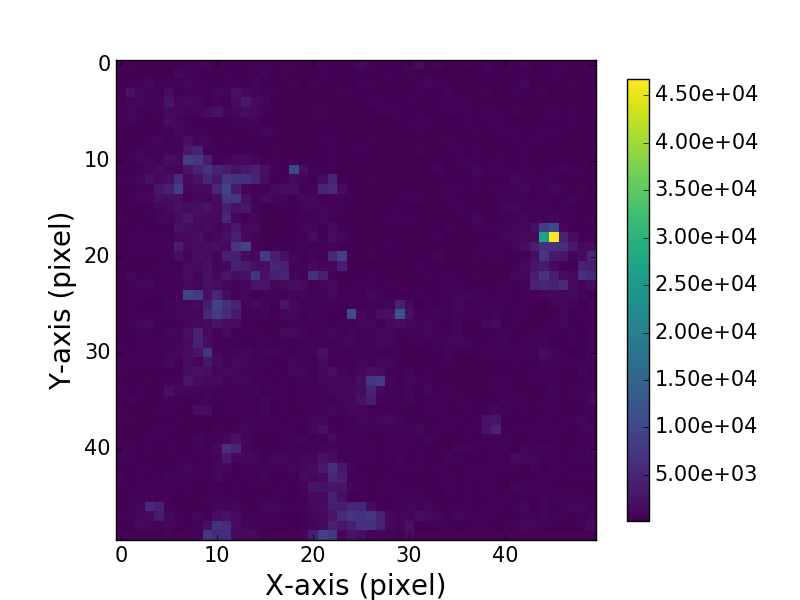
\includegraphics[trim = 0 0 0 0,  clip= true, width = \pairplotwide]{./pics/scan_xy-02_2APD.png}}
			\caption{}
			\label{subfig::scan_1}
		\end{subfigure}
		\hfill
		\begin{subfigure}{ 0.49\linewidth}
			\centering
			\testbox{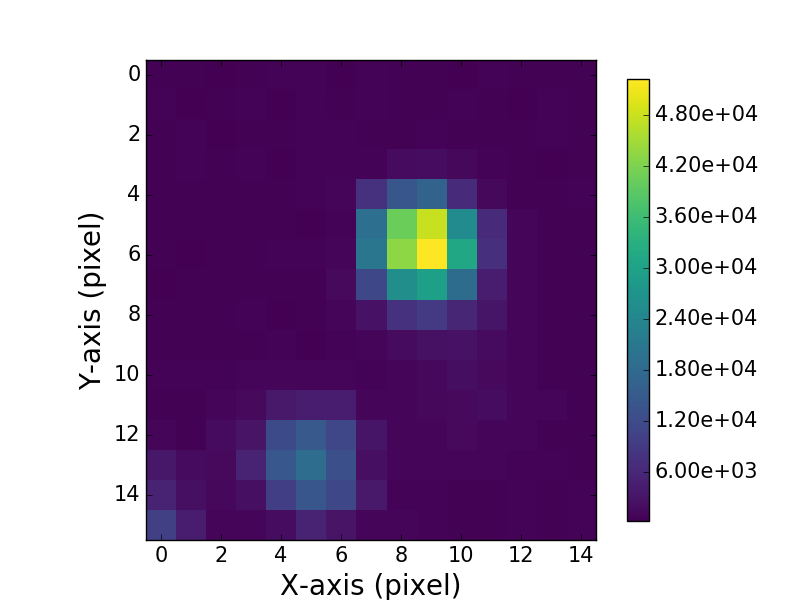
\includegraphics[trim = 0 0 0 0,  clip= true, width = \pairplotwide]{./pics/scan_xy-05_2APD.png}}
			\caption{}
			\label{subfig::scan_2}
		\end{subfigure}
		\caption[Confocal \pl scans]{\Pl scans measured in the confocal setup. (a) depicts an overview of a size of $\SI{50}{\micro\meter}\times\SI{50}{\micro\meter}$, The bright yellow dot is emitter \embroad introduced in this chapter. Also several of the not so intense emitter visible as light blue spots were investigated. (b) Shows a detail scan of a size of $\SI{8}{\micro\meter}\times\SI{7.5}{\micro\meter}$ of \embroad.}
		\label{fig::scans}
	\end{figure}

	\FloatBarrier	

\subsection{\Zpl}\label{subsec::zpl}

	The \cwl and the \lw of the \zpl (\ZPL) of \siv luminescence spectra for samples \insituF, \insituS, and \insituH are determined by fitting a Lorentzian fit to the \ZPL.
	Both spectra from \nds containing single and multiple \sivs are taken into account.
	\Fref{fig::various_spectra} depicts a few examples of the measured spectra in order show how diverse they are.

	\begin{figure}[!htb]
		\begin{subfigure}[t]{ 0.49\linewidth}
			\centering
			\testbox{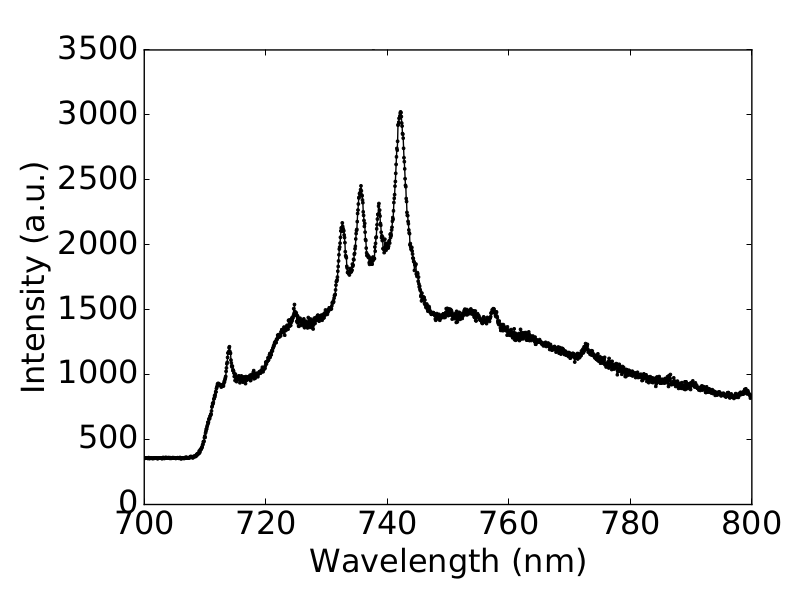
\includegraphics[trim = 0 0 0 0,  clip= true, width = \pairplotwide]{./pics/spectrum11.png}}
			\caption{}
			\label{subfig::spectrum_1}
		\end{subfigure}
		\hfill
		\begin{subfigure}[t]{ 0.49\linewidth}
			\centering
			\testbox{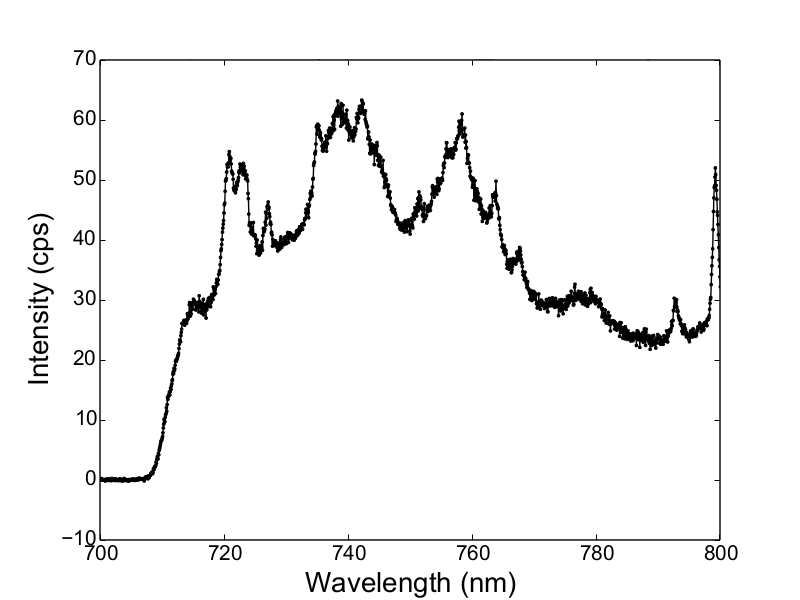
\includegraphics[trim = 0 0 0 0,  clip= true, width = \pairplotwide]{./pics/Spektrum3_t=30s.png}}
			\caption{}
			\label{subfig::spectrum_2}
		\end{subfigure}
		\hfill
		\begin{subfigure}[t]{ 0.49\linewidth}
			\centering
			\testbox{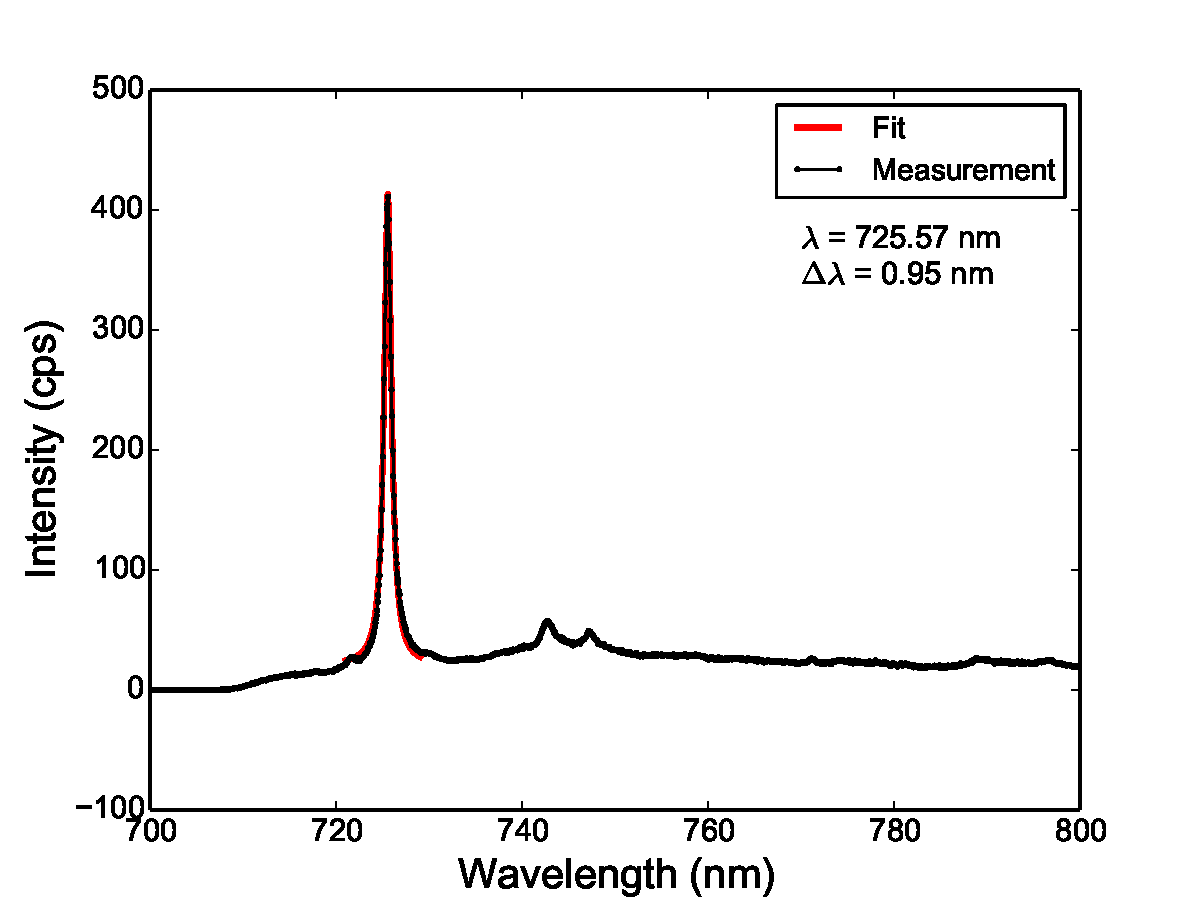
\includegraphics[trim = 0 0 0 0,  clip= true, width = \pairplotwide]{./pics/Spektrum2_2_t=30s_alt.pdf}}
			\caption{}
			\label{subfig::spectrum_3}
		\end{subfigure}
		\hfill
		\begin{subfigure}[t]{ 0.49\linewidth}
			\centering
			\testbox{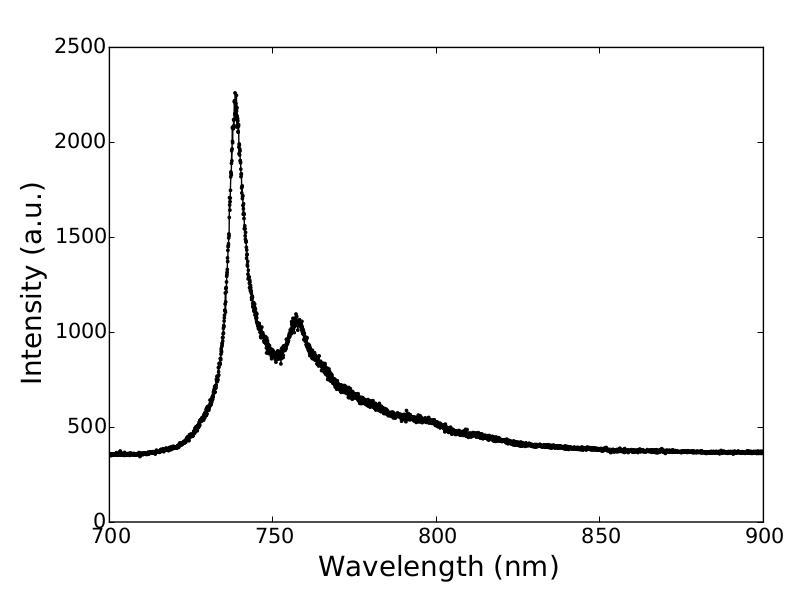
\includegraphics[trim = 0 0 0 0,  clip= true, width = \pairplotwide]{./pics/plot_spe_scan_xy-39x8y9_300uW_t120.png}}
			\caption{}
			\label{subfig::spectrum_4}
		\end{subfigure}
		\hfill
		\begin{subfigure}[t]{ 0.49\linewidth}
			\centering
			\testbox{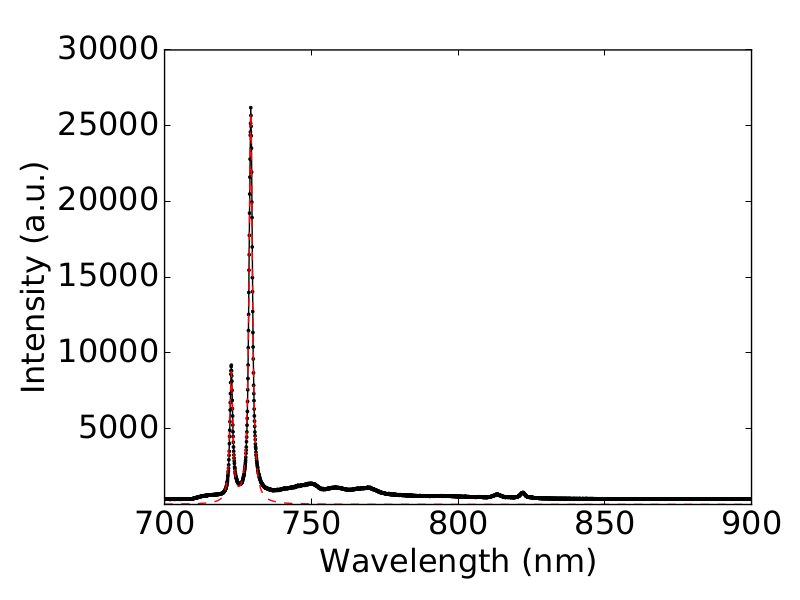
\includegraphics[trim = 0 0 0 0,  clip= true, width = \pairplotwide]{./pics/spectrum_scan_xy-40x4y4_392uW_t10_fit.png}}
			\caption{}
			\label{subfig::spectrum_5}
		\end{subfigure}
		\hfill
		\begin{subfigure}[t]{ 0.49\linewidth}
			\centering
			\testbox{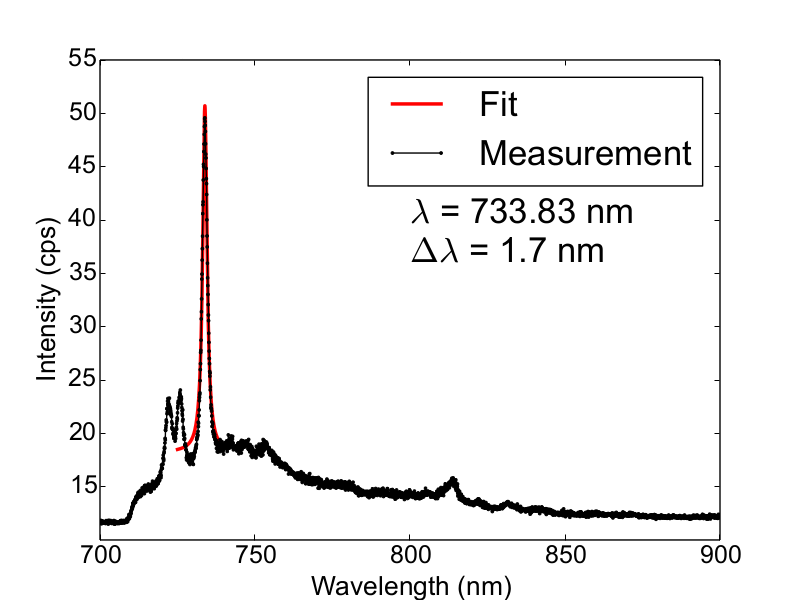
\includegraphics[trim = 0 0 0 0,  clip= true, width = \pairplotwide]{./pics/spectrum_scan_xy-21_2_t30_380uW.png}}
			\caption{}
			\label{subfig::spectrum_6}
		\end{subfigure}
		\caption[Overview of diversity of \siv spectra.]{Various spectra of samples consisting of wet-milled \nds with \textit{in-situ} incorporated \sivs. The \nds yielding spectra (a) and (b) host many \sivs with \ZPL at different \cwls. (c) and (d) exhibit one dominant \ZPL and recognizeable sideband features. In (e) two \ZPLs of different intensity are visible, in (f) one \ZPL donminates the spectrum while some \ZPLs of lower intensity are present.}
		\label{fig::various_spectra}
	\end{figure}

	In \Fref{fig::bimodal_distr} the \lw for each measured \ZPL is plotted against its \cwl.

	\begin{figure}[!htb]
			\centering
			\testbox{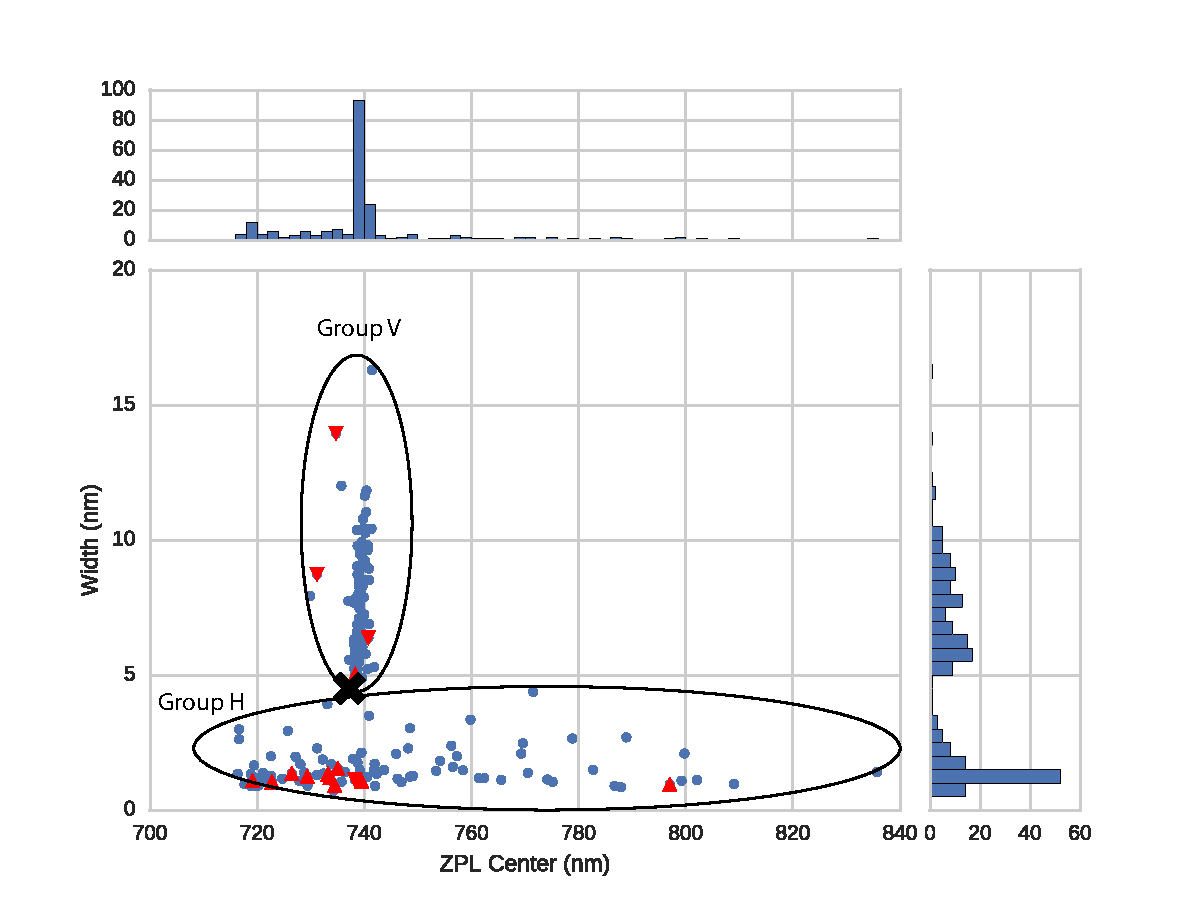
\includegraphics[trim = 0 0 0 0,  clip= true, width = \oneimagewide]{./pics/distro_histo_sarah.pdf}}
			\caption[Spectral distribution of \siv \ZPLs]{Distribution of the \ZPL \cwl versus the \lw of the \ZPL of the investigated \sivs in milled \nds containing \textit{in-situ} incorporated \sivs for samples \insituF, \insituS, \insituH{}. The data separates into a horizontal (\hl) and a vertical (\vl) cluster. The bold black cross marks the position of an ideal \siv in unstrained bulk diamond \cite{Arend2016a}. The red triangles indicate emitters with an anti-bunching dip in the \gtz measurement. Upwards pointing triangles represent blinking emitters (fluorescence intermittency), while triangles pointing down represent non-blinking emitters (see \Fref{subsec::photostab}).}
			\label{fig::bimodal_distr}
	\end{figure}

	What immediately strikes the eye is a pattern that to our knowledge has not been reported to date:
	The observed \ZPLs partition into two groups, denoted a horizontal cluster (\hl) and a vertical cluster (\vl). The two clusters are separated by a gap, i.e.\ a region with a pronounced lack of data points.
	Single emitters are identified both in \hl and \vl, marked as red triangles in \Fref{fig::bimodal_distr}. Further details on single emitters are given in section \Fref{subsec::g2}.
	\\
	The two groups are defined by their characteristic \cwls and \lws:
	In \hl very prominent \ZPL peaks are found showing \lws in the range of \SIrange{1}{5}{nm} and \cwls in the range of \SIrange{715}{835}{nm}.
	\Fref{subfig::emnarrow} shows a representative spectrum of a single emitter in \hl (denoted \emnarrow), exhibiting a \ZPL line width of \SI{1.4}{nm} and a \cwl of \SI{726.5}{nm}.
	In contrast, in \vl, the spectra exhibit broader \ZPL \lws of approximately \SI{5}{nm} up to \SI{18}{nm}.
	Their \ZPL \cwls, however, are distributed within the very narrow range of \SIrange{738}{741}{nm}.
	\Fref{subfig::embroad} shows a spectrum of a single emitter of \vl (denoted \embroad) with a ZPL \lw of \SI{6.4}{nm} and a \cwl of \SI{740.8}{nm}.
	For comparison, the room temperature ZPL of \sivs in unstrained bulk diamond exhibits a \lw of \SIrange{4}{5}{nm} and a \cwl of \SI{737.2}{nm} marked with a black cross in \Fref{fig::bimodal_distr} \cite{Arend2016a,Dietrich2014}.

	\begin{figure}[!htb]
		\begin{subfigure}{0.5\linewidth}
			\centering
			\testbox{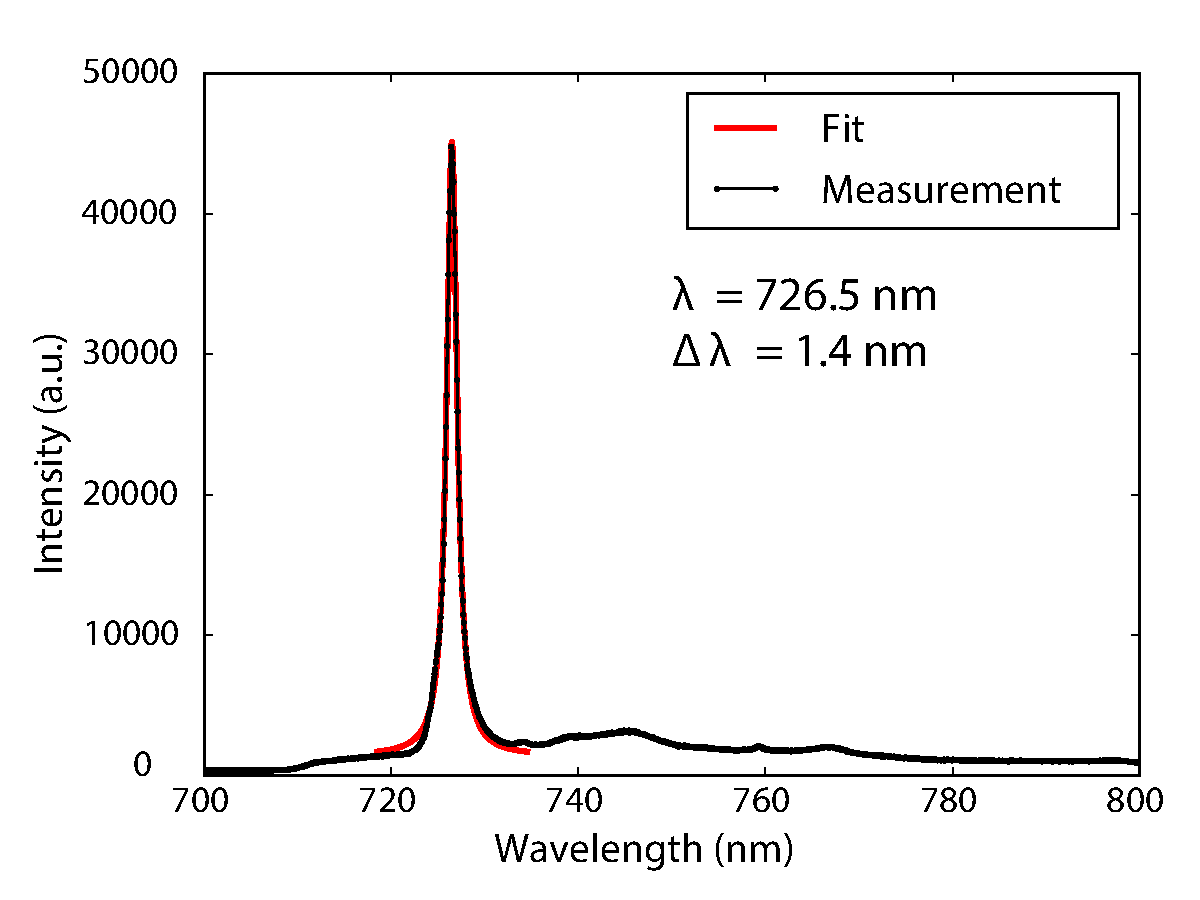
\includegraphics[trim = 0 0 0 0 , clip = true, width = \pairplotwide]{./pics/Ir8_Spektrum_8_notitle.pdf}}
			\caption{}\label{subfig::emnarrow}
		\end{subfigure}
		\hfill
		\begin{subfigure}{0.5\linewidth}
			\centering
			\testbox{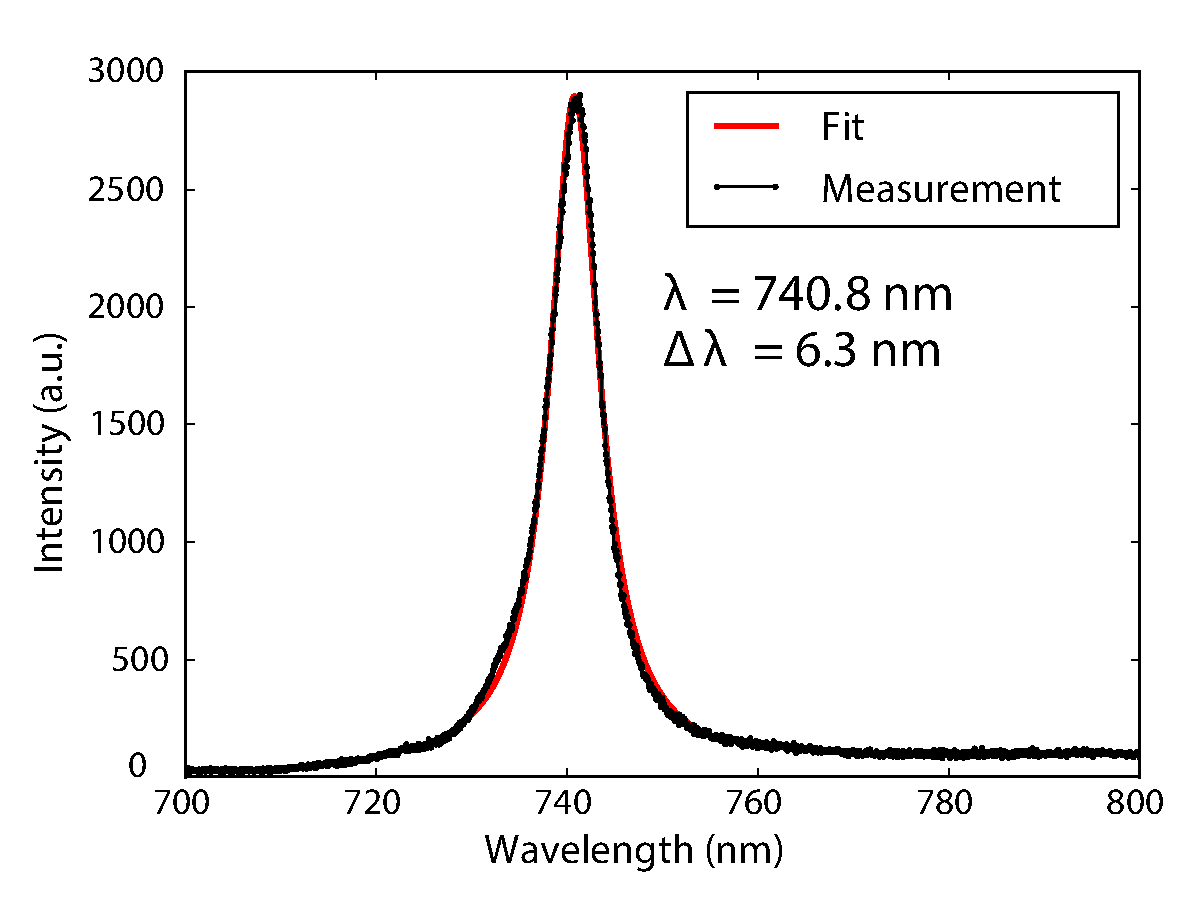
\includegraphics[trim = 0 0 0 0,  clip = true, width = \pairplotwide]{./pics/Ir8_scan_xy05_199uW_t30_notitle.pdf}}
			\caption{}\label{subfig::embroad}
		\end{subfigure}
		\caption[Sample \siv \pl spectra for \vl and \hl]{Representative photoluminescence spectra of sample \insituHao measured at room temperature. (a) Spectrum of \hl of \Fref{fig::bimodal_distr}, denoted \emnarrow. (b) Spectrum of \vl of \Fref{fig::bimodal_distr}, denoted \embroad. The red lines are Lorentzian fits to the peaks.}
		\label{fig::spectra}
	\end{figure}

	To determine how much the \ZPLs contribute to the total observed emission of \emnarrow and \embroad, we determine the \db factors for both.
	The \db factor is defined by $DW = I_{ZPL}/I_{TOT}$ and is therefore suited as a measure for sideband intensity.
	The \db factor for \emnarrow amounts to \num[separate-uncertainty]{0.81(1)} (given uncertainty due to fit).
	This \db factor corresponds to a \hr factor $S =- \ln{(DW)}$ \cite{Walker1979} of \num[separate-uncertainty]{0.21(1)}, which is in good agreement with the values reported in \cite{Neu2011b}.
	The error is mainly due to background corrections.
	When zooming in onto the spectrum of \embroad we do not find distinct sidebands peaks, i.e.\ almost all emission for this emitter is focused into the \ZPL.
	Considering resolution limits of the spectrometer, dark-counts and fluorescence background, we evaluate the \db factor to be larger than \num[separate-uncertainty]{0.97}.
	It is the largest \db factor amongst all our milled \sivs.
	The two mentioned \db factors should not be interpreted as single representative emitters for the respective groups, they rather serve as an orientation of the spread of the \db factors of both groups.
	It has to be pointed out, that we did not find any systematic difference of the \db factor between \hl and \vl.
	
	To provide context for the novel findings presented in \Fref{fig::bimodal_distr}, we compare our results to various earlier findings.
	Furthermore, we discuss an additional comparison to an investigated control sample fabricated using \si implantation.
	The results are presented in \Fref{fig::bimodal_distr_compare}.


	\begin{figure}[!htb]
		\centering
		\testbox{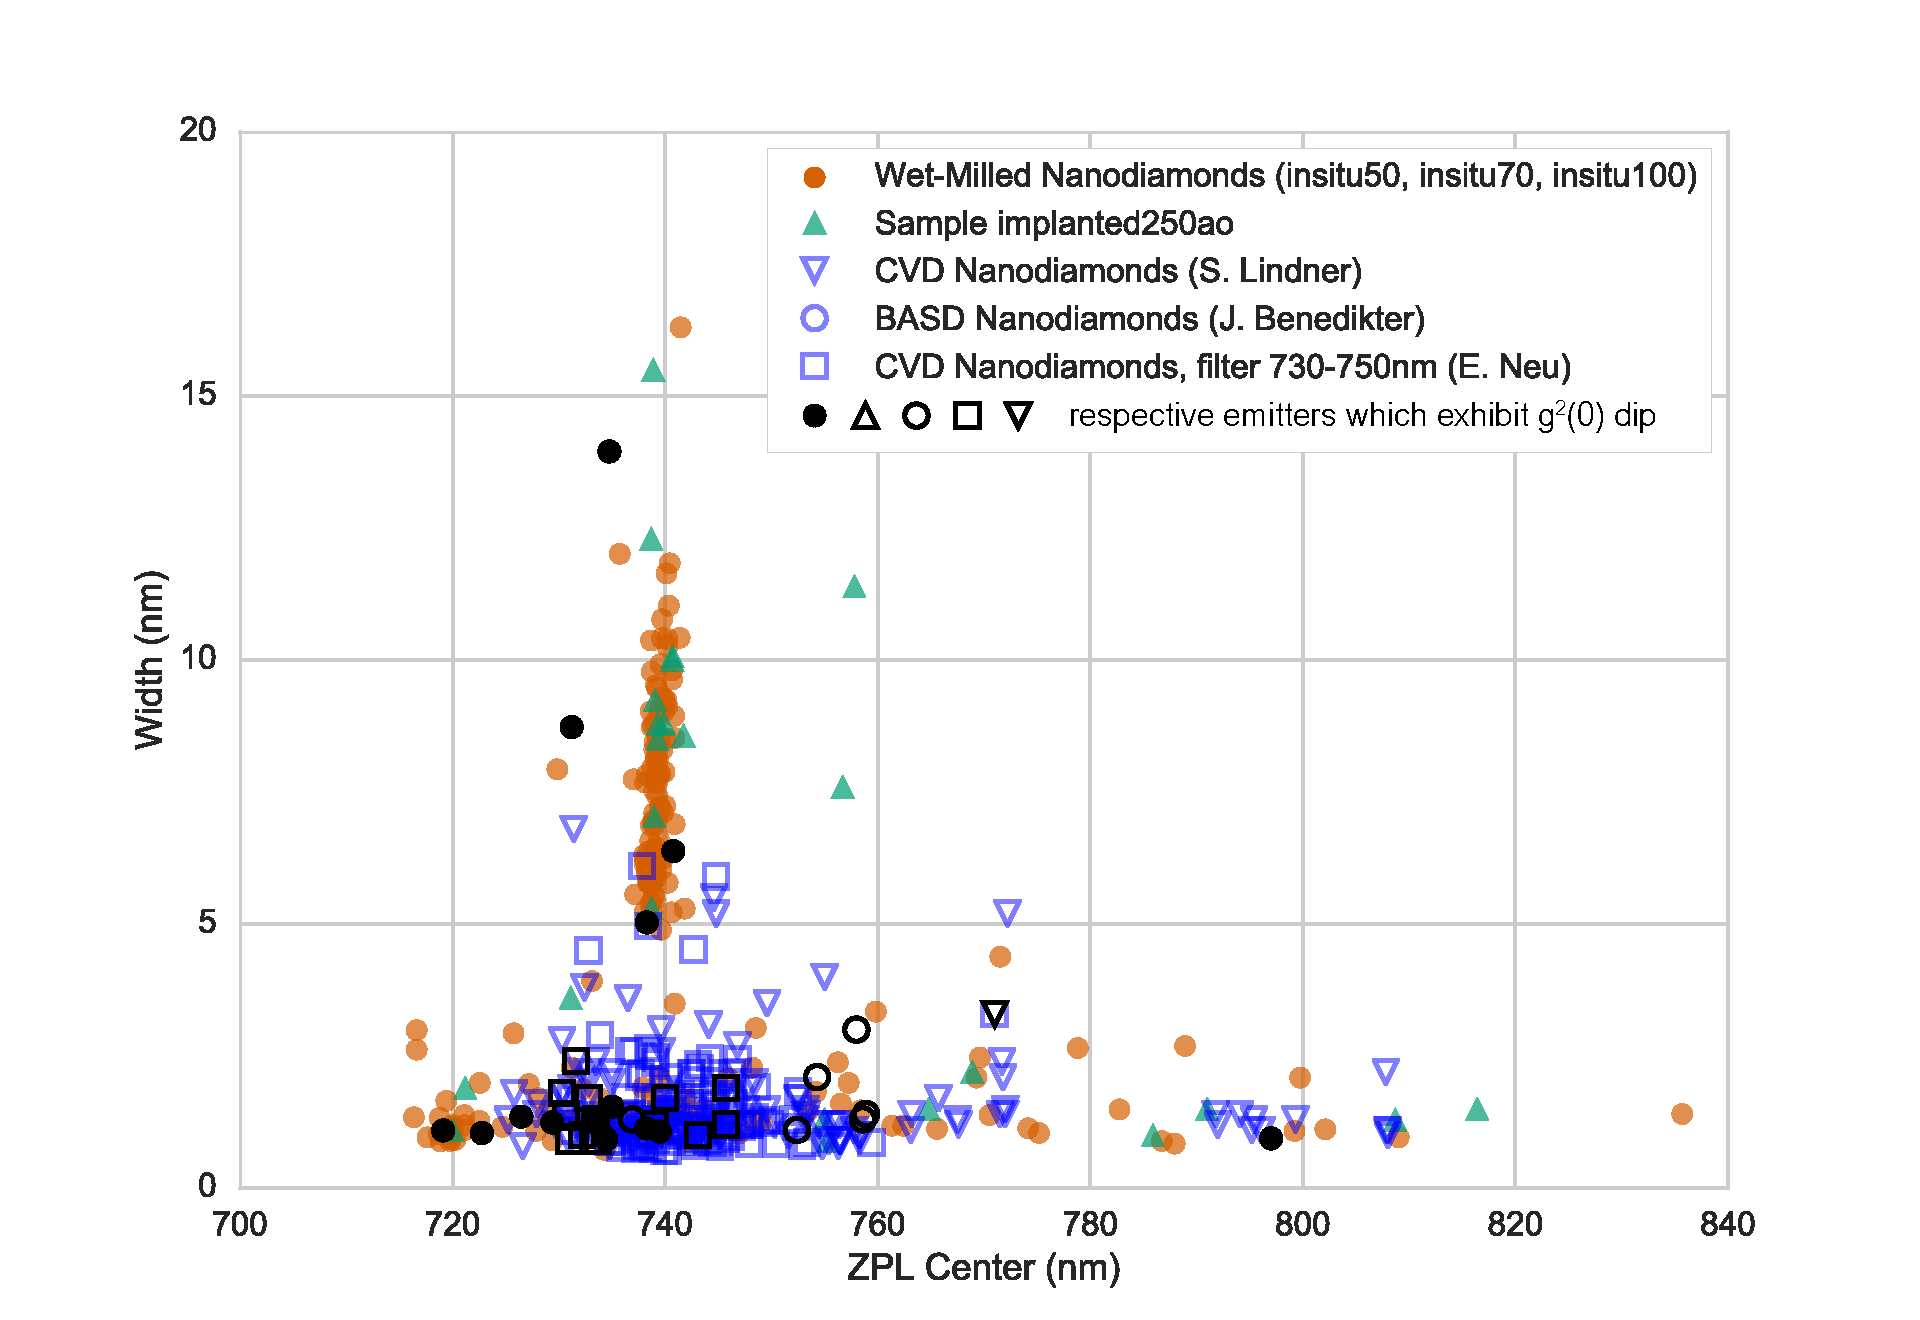
\includegraphics[trim = 0 0 0 0,  clip= true, width = \oneimagewide]{./pics/distro_alldata_three_colors_legend.pdf}}
		\caption[Comparison of \siv \lws with available data sources]{Comparison of the distribution of the \lw vs. the center wavelength of the ZPL of the investigated \sivs in milled \nds (samples \insituF, \insituS, \insituH) with data measured on sample \implantedTao (implanted with \Si); with data measured in our group on CVD \nds produced by M. Schreck \cite{Neu2011b}; with data measured on \nds reported by J. Benedikter in \cite{Benedikter2017a}; and with data measured in CVD diamonds by E. Neu in a filter window between \SIlist{730; 750}{nm} \cite{Neu2012}. Black symbols represent emitters exhibiting a dip in the \gtz function, indicating a single or very few \sivs}
		\label{fig::bimodal_distr_compare}
	\end{figure}


	Samples for which previous data has been taken are:
	\begin{enumerate}
		\item \nds produced by \basd (BASD) of polycrystalline \CVD diamond films (blue rings in \Fref{fig::bimodal_distr_compare} \cite{Neu2011a}; data taken from \cite{Benedikter2017a}).
		\item \label{item::elke_cvd}\nds produced by heteroepitaxial \CVD growth on \ir substrates with \textit{in-situ} incorporated \sivs; measured in a spectral filter window of \SIrange{730}{750}{nm} (blue squares in \Fref{fig::bimodal_distr_compare}; data reused from \cite{Neu2012} with permission).
		\item \nds produced in the same manner as in \ref{item::elke_cvd} (blue downwards pointing triangles in \Fref{fig::bimodal_distr_compare}; produced by M. Schreck \cite{Neu2011b}; spectroscopic measurement performed with setup described in \Fref{sec::confocal}).
	\end{enumerate}
	
	All previous data from different \nd material fit nicely with the \ZPL distribution presented in \Fref{fig::bimodal_distr_compare}, confirming the findings of \Fref{fig::bimodal_distr}.
	\\
	We verify that the observed luminescent defects are indeed \si related by performing control experiments with \si implanted samples (sample \implantedTao).
	By doing so we rule out the possibility that the two clusters in the distribution are a result of artifacts.
	Such artifacts include other elements incorporated into the \nds during the growth process: Residue from previous processes performed in the diamond growth chamber or material from chamber parts may be incorporated during \nd growth.
	\Fref{fig::bimodal_distr_compare} shows that the implanted \sivs cover roughly the same spectral range as the \textit{in-situ} incorporated centers from around \SIrange{720}{820}{nm} as the \textit{in-situ} incorporated centers.
	This correlation provides strong evidence for the \si related origin of the defects.
	
	% In the next paragraphs, the \ZPL distribution will be discussed in further detail.
	To provide a theoretical interpretation, the \ZPL \cwl shift is investigated in further detail and compared to results from density functional calculations.
	Zooming in to \vl (\Fref{subfig::distro_inset1}) it becomes clear that only six of the measured data points in \vl are situated at a shorter \cwl than the point attributed to an ideal \siv in unstrained bulk material.
	The the shortest wavelength shift is at \SI{729.9}{nm}.
	At the same time, much more data exhibit a \cwl bigger than the ideal \siv.
	This asymmetry suggests that a red-shift of the \ZPL of an \siv is significantly more likely than a blue-shift.

		\begin{figure}[!htb]
			\begin{subfigure}{.5\textwidth}
				\centering
				\testbox{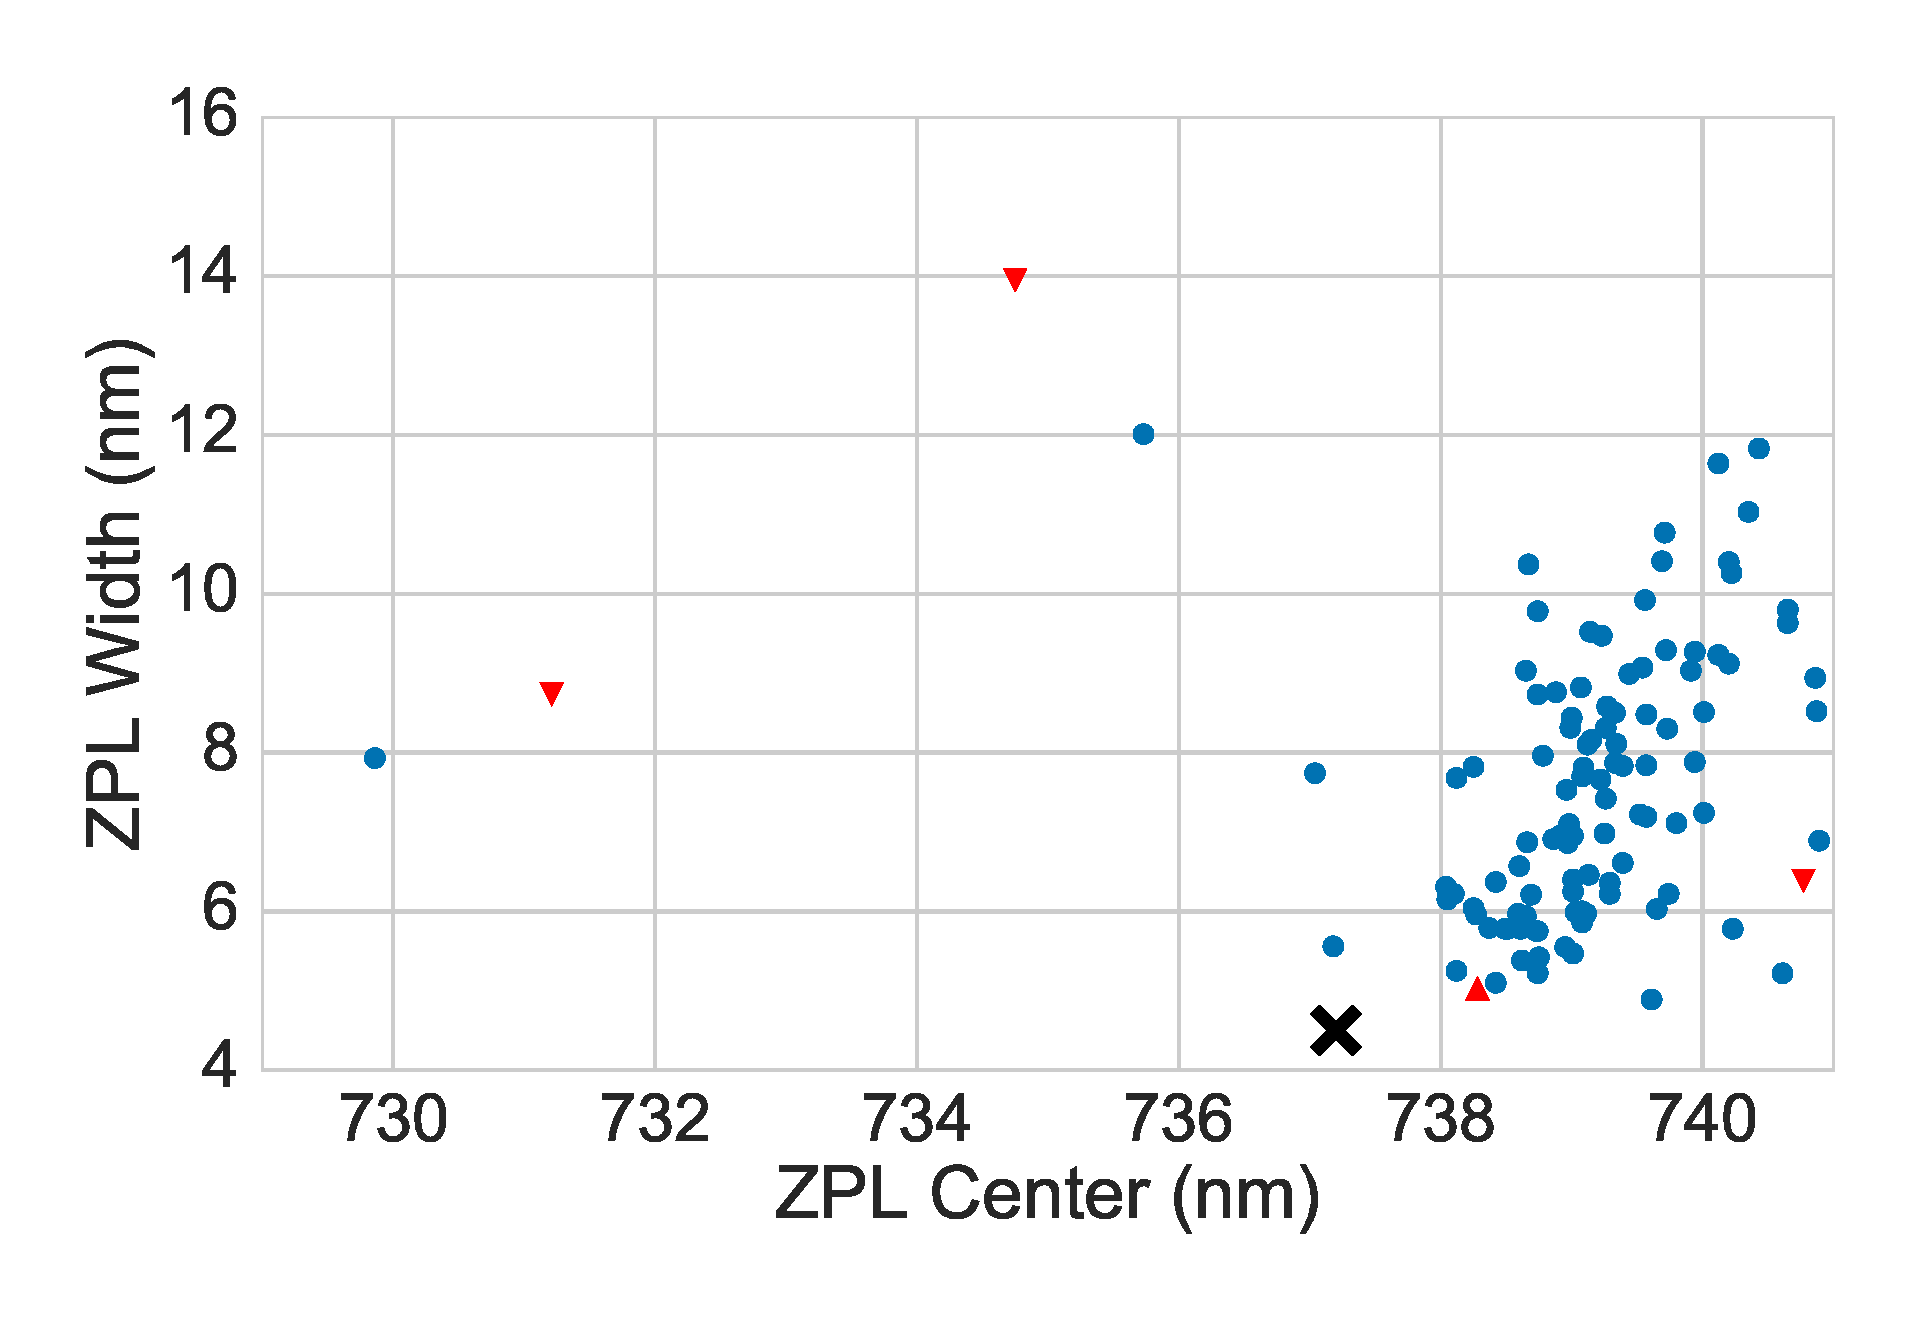
\includegraphics[trim = 0 0 0 0,  clip= true, width=\pairplotwide]{./pics/paper_inset_line_statistics_nofit.pdf}}
				\caption{}
				\label{subfig::distro_inset1}
			\end{subfigure}
			\begin{subfigure}{.5\textwidth}
				\centering
				\testbox{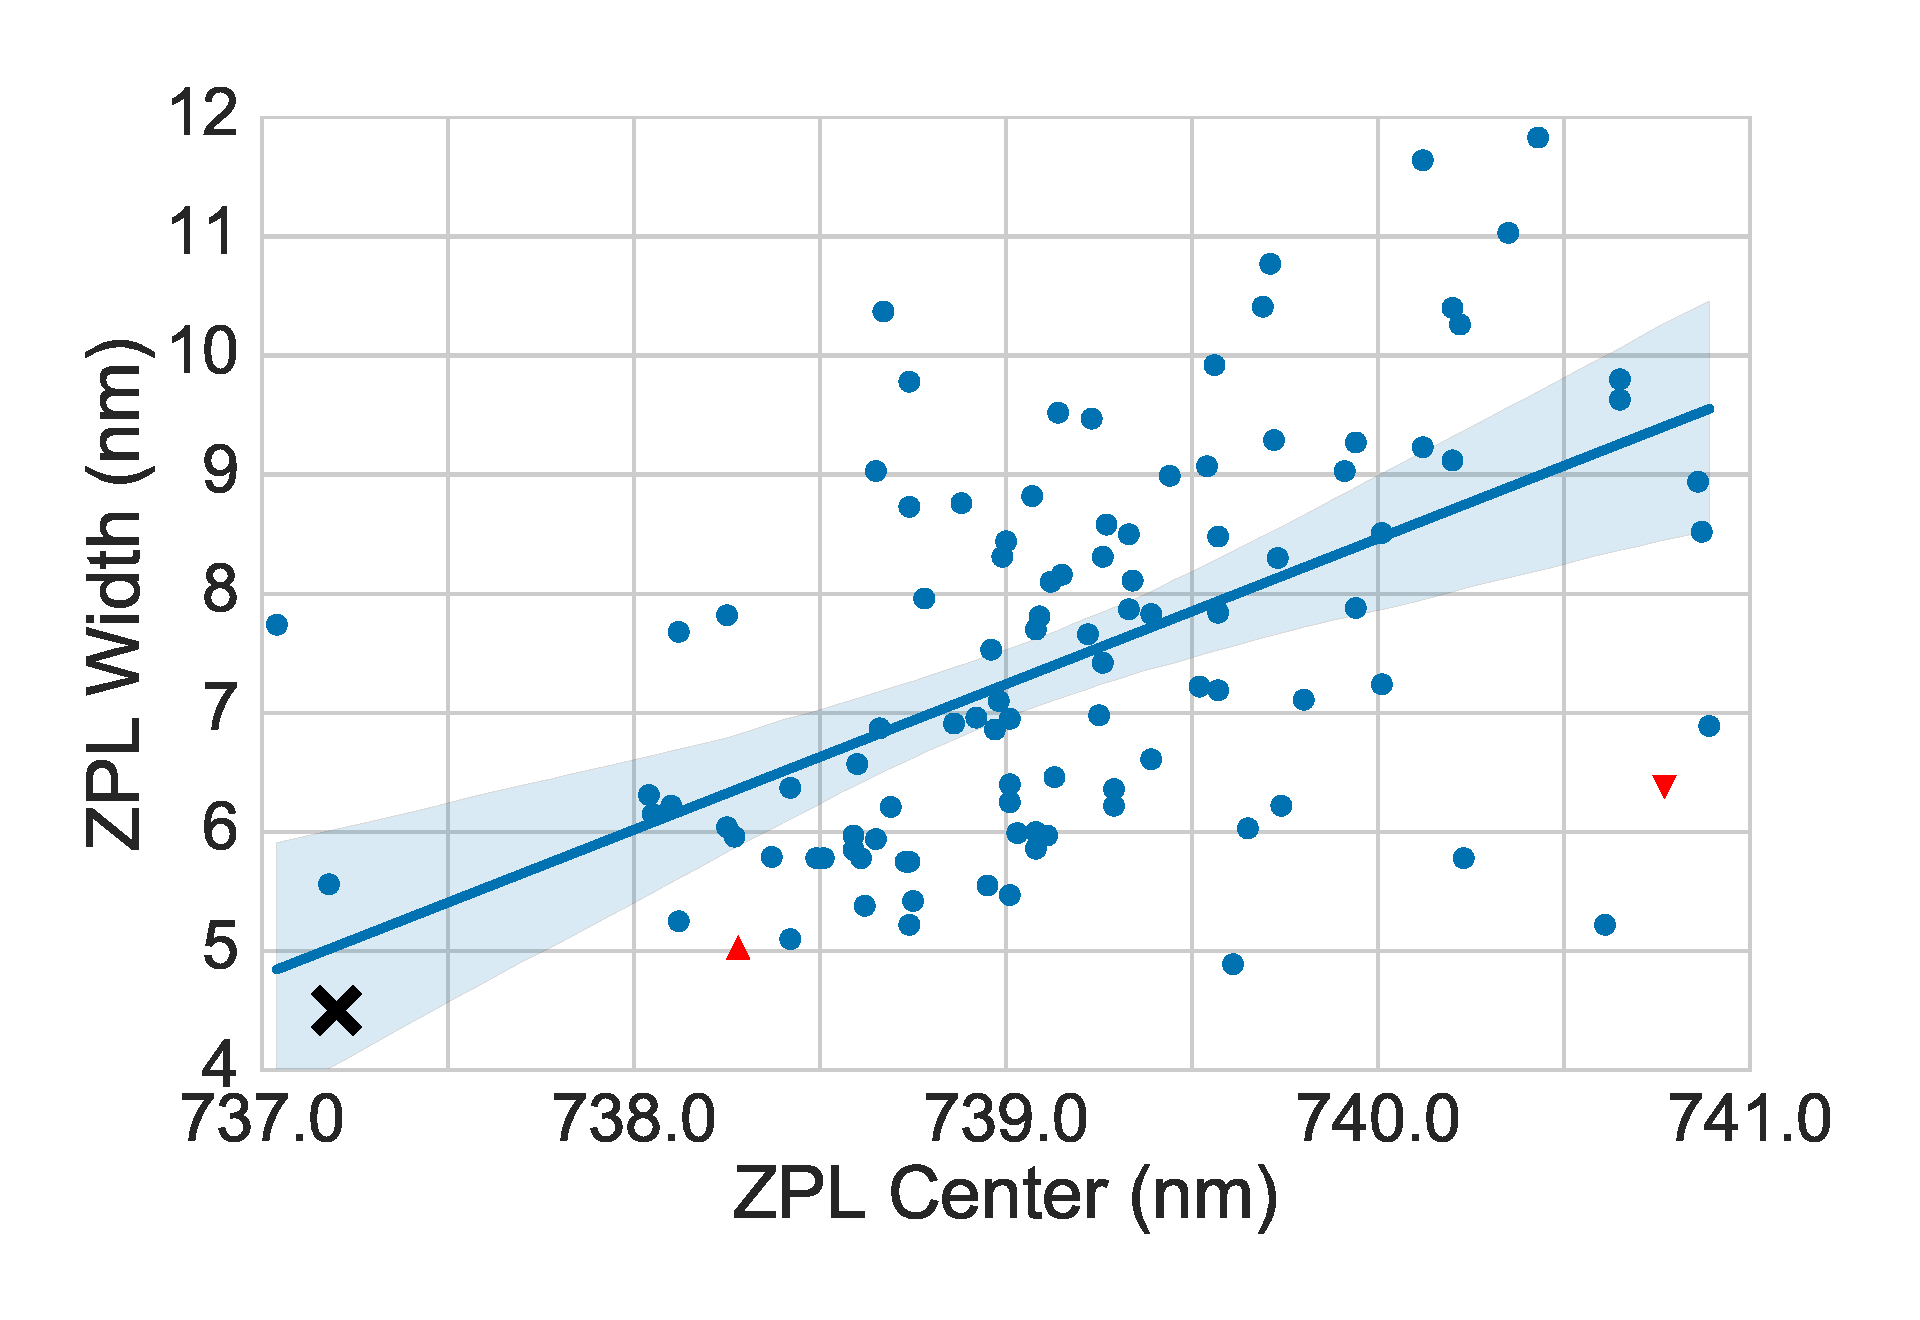
\includegraphics[trim = 0 0 0 0,  clip= true, width=\pairplotwide]{./pics/paper_line_statistics_regression.pdf}}
				\caption{}
				\label{subfig::distro_inset2}
			\end{subfigure}
			\caption[Zoom-in onto \sivs of the \vl]{(a) A zoom into \vl. While many data points exhibit higher \cwls (i.e. a redshift) than the ideal \siv in bulk, only few exhibit shorter \cwls (i.e. a blue-shift). (b) Zooming further into \vl, a clear trend of broader \ZPL \lws for larger \ZPL center shifts is visible. The line in a linear regression to all data points between \SIlist{737;741}{\nano\meter} which exhibit a \lw bigger than \SI{4}{\nano\meter}.}
			\label{fig::bimodal_distr_zoom}
		\end{figure}

	Several mechanisms contribute to the \cwl shift, predominantly hydrostatic- and material strain.
	As explained in \Fref{subsec::raman_strain}, we measured the Raman shift of samples \insituS and \implantedTao.
	These measurements indicate strain in the diamond lattice in the range of \SIrange{-8.56}{4.26}{\giga\pascal}.
	\Fref{fig::stress_pressure} shows results from density functional calculations.
	The shift of the  \ZPL is modeled in dependence of pressure in the diamond lattice both for hydrostatic stress and for uniaxial stress.
	\Fref{fig::stress_pressure} illustrates that the assumption stated in \Fref{subsec::raman_strain}, namely that the strain in the \nds is due to hydrostatic and uniaxial stress, corresponds well with the measured \ZPL shifts in \vl.

		\begin{figure}[!htb]
			\centering
			\testbox{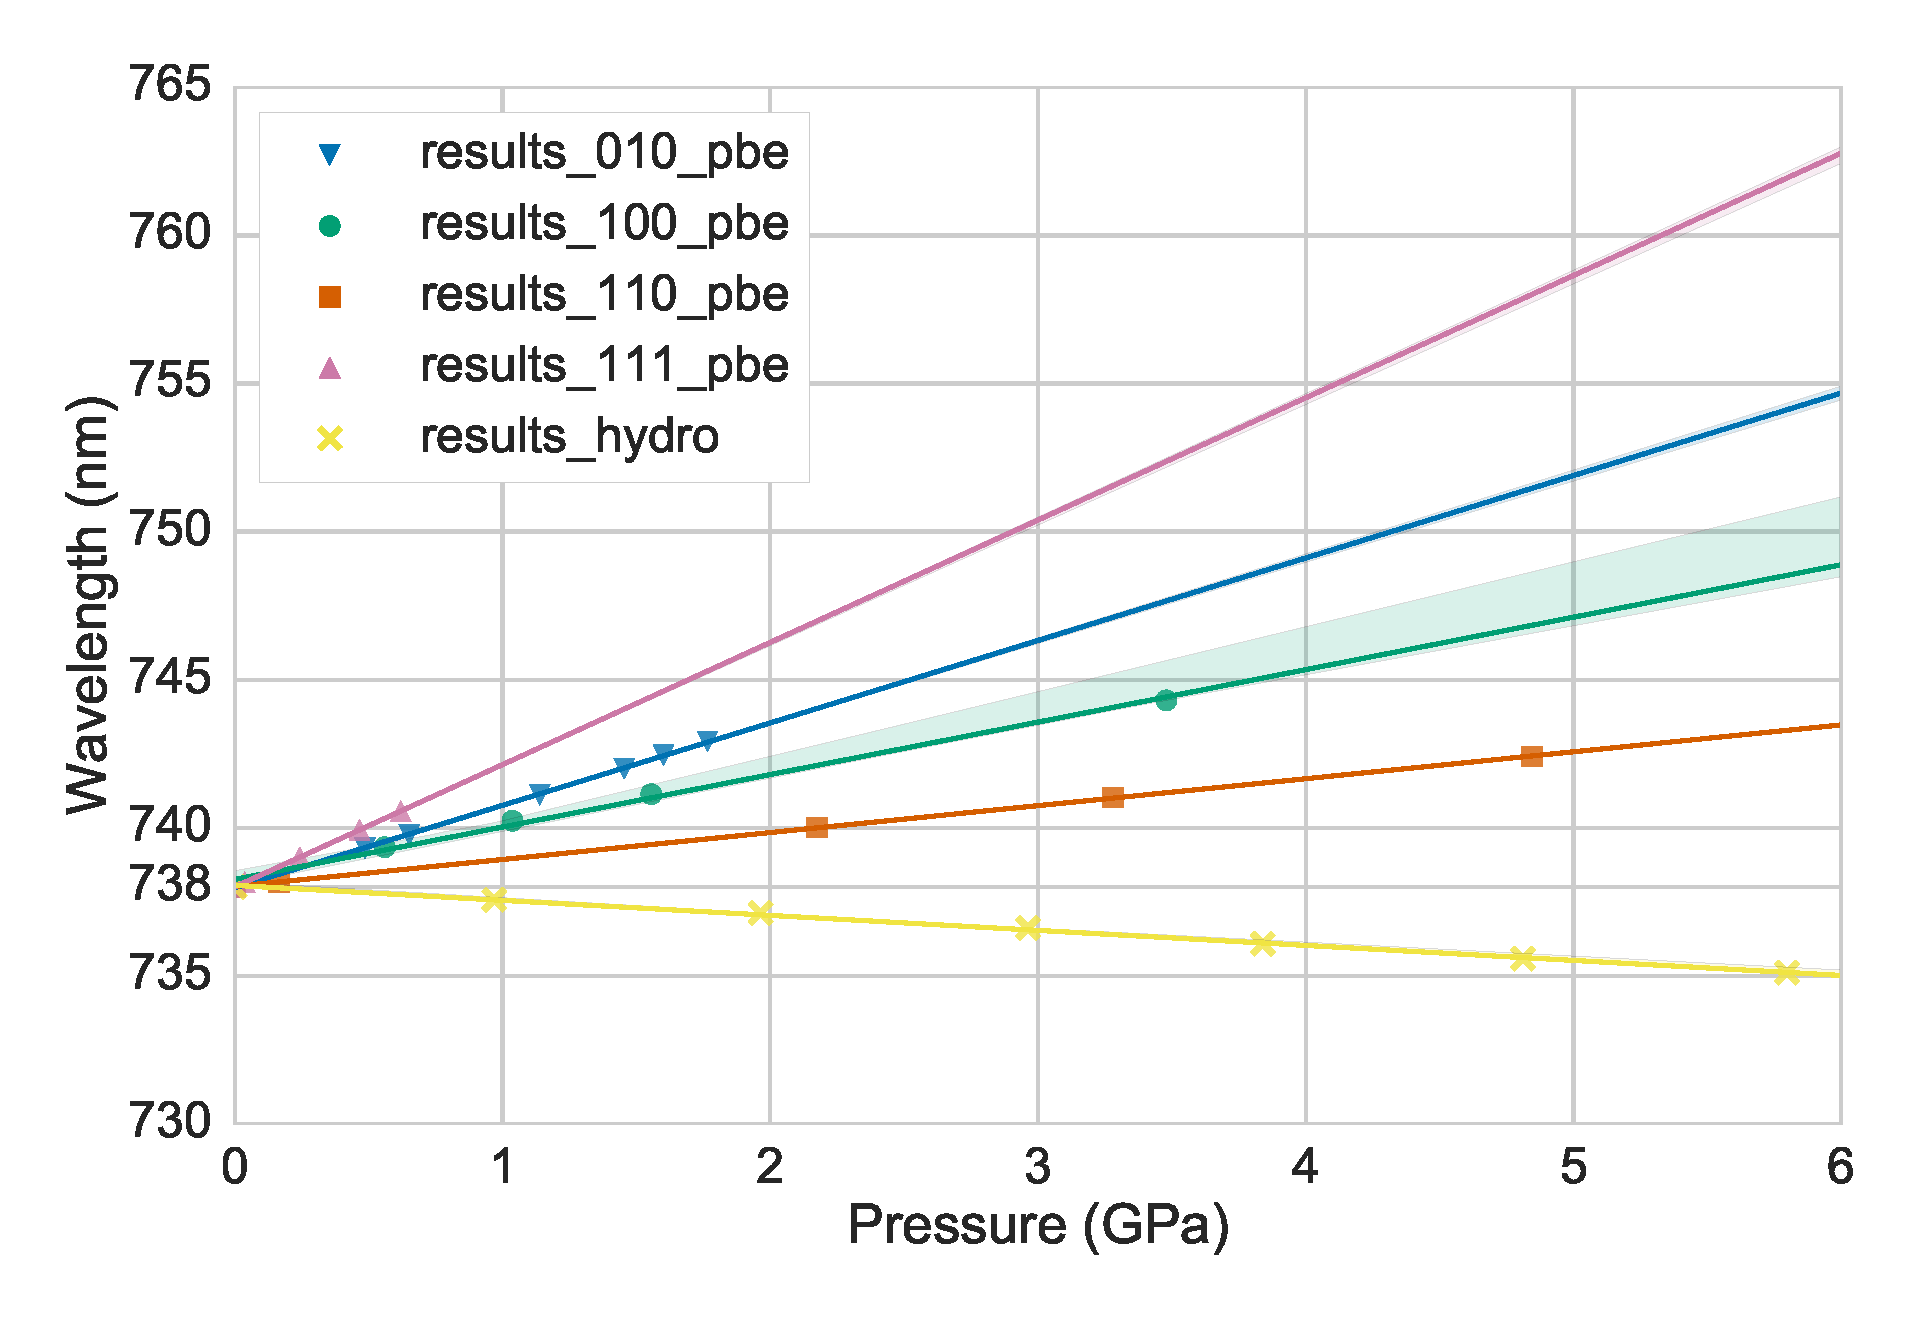
\includegraphics[trim = 0 0 0 0,  clip= true, width = 0.6\linewidth]{./pics/adam_gali_big_labels.pdf}}
			\caption[Calculated dependence between \siv \ZPL and lattice pressure]{Calculations of the wavelength of the \siv \ZPL in dependence of pressure. Markers: calculated pressure with PBE functional; Lines: linear fits to the calculated points, the shaded area around the lines representing the one sigma (68\%) confidence interval. Yellow: hydrostatic pressure; other colors: uniaxial pressure, for different orientations. All calculations are performed with a PBE functional. Hydrostatic-type pressure causes a moderate blue shift whereas uniaxial strain causes larger redshift with different magnitudes depending on the direction of the strain}
			\label{fig::stress_pressure}
		\end{figure}

	With higher uniaxial pressure, the \ZPL becomes more and more red-shifted.
	The blue shifted \ZPL \cwls are explained by hydrostatic stress in the diamond material.
	The strain calculated from the Raman measurements corresponds well with the results in \Fref{fig::stress_pressure} for \vl.
	However, the measured shifts in \hl are too broad to be solely explained by strain in the diamond.
	A potential explanation for the very broad distribution of defect center \ZPL \cwls could be the association of \sivs with a further nearby defect, such as a vacancy, or a modified SiV complex such as SiV:H \cite{Thiering2015}.
	\\
	Zooming in to \vl, another effect becomes visible (\Fref{subfig::distro_inset2}):
	With increasing  \ZPL \cwl, the \lw becomes broader.
	As discussed above, a red-shift of the \ZPL is linked to increasing uniaxial strain.
	Thus we conclude that the \ZPL \lw too is affected by strain in the diamond lattice.
	Here, a modified electron-phonon coupling \cite{Jahnke2015a} causes increased uniaxial stress, resulting in larger \lws.
	A similar effect has been previously observed for \sivs at cryogenic temperatures \cite{Arend2016a}.
	\\
	To conclude, we are able to explain the distribution of \ZPL \cwls in \vl very consistently with theoretical predictions based on perturbative shifts due to strain in the diamond lattice.
	On the other hand, we have to assume that \hl is comprised of modified \sivs, the structure of which is currently unclear.

	%!TEX root = ../../../main.tex

	\subsection{Sideband} \label{subsubsec::sideband}

		It is known that the \pl spectra of \sivs in \nd are dominated by the \zpl. As a result \psb contributions remain small, a fact expressed in large \db factors of over \SI{70}{\percent} established previously \cite{Neu2011,Neu2011b}. Our own measurements are consistent with these of \emnarrow and \embroad results. We also find distinct sideband peaks in many \siv \pl emission spectra.
		The investigated emitters exhibit two different structures of sideband spectra: The spectra in \vl exhibit one strong sideband peak, spectra in \hl exhibit several weaker sideband peaks. \Fref{subfig::sideband_group_v} and \Fref{subfig::sideband_group_h} illustrate the respective observations.

		\begin{figure}[!htb]
			\begin{subfigure}{0.49\linewidth}
				\centering
				\testbox{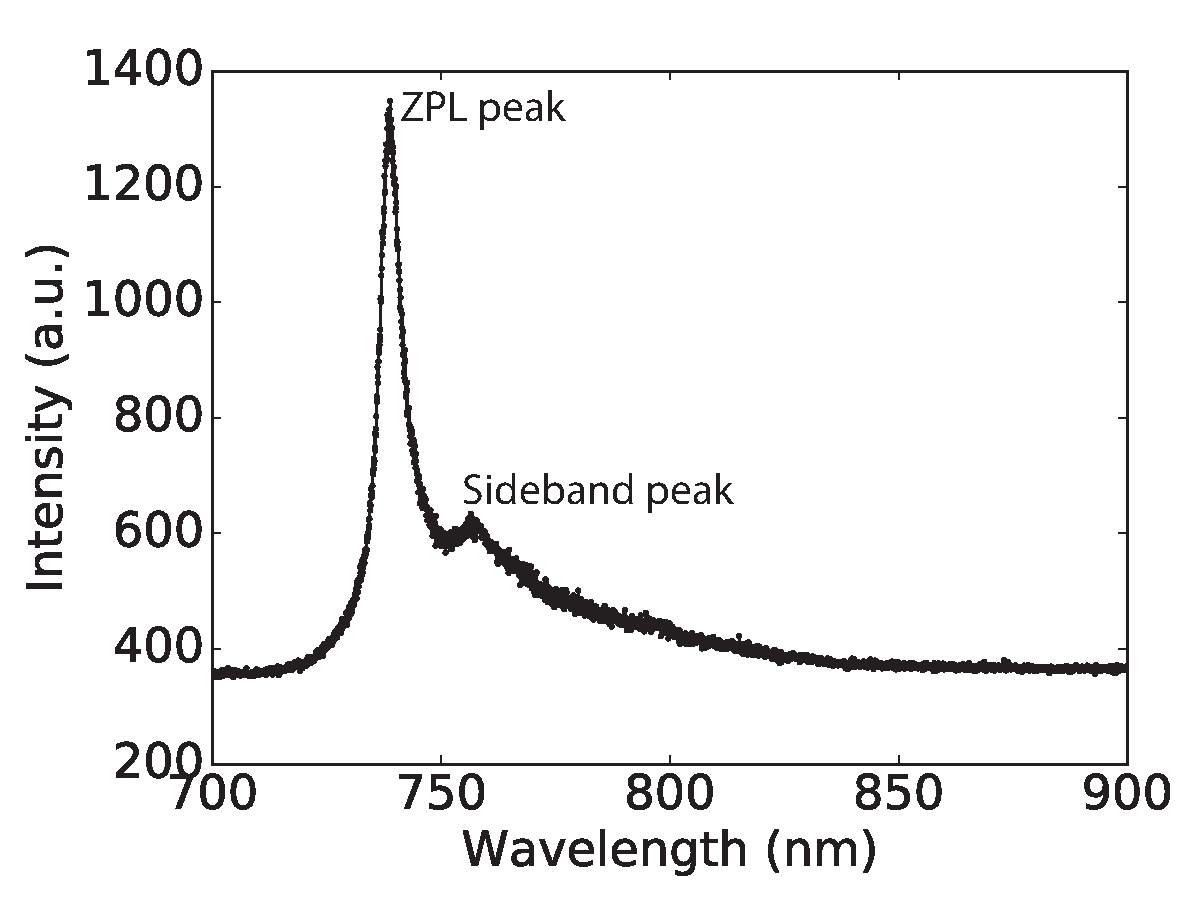
\includegraphics[trim = 0 0 0 0,  clip= true, width = \pairplotwide]{./pics/Ir25M_spe_scan_xy-38x9y16_300uW_t120.pdf}}
				\caption{}
				\label{subfig::sideband_group_v}
			\end{subfigure}
			\hfill
			\begin{subfigure}{0.49\linewidth}
				\centering
				\testbox{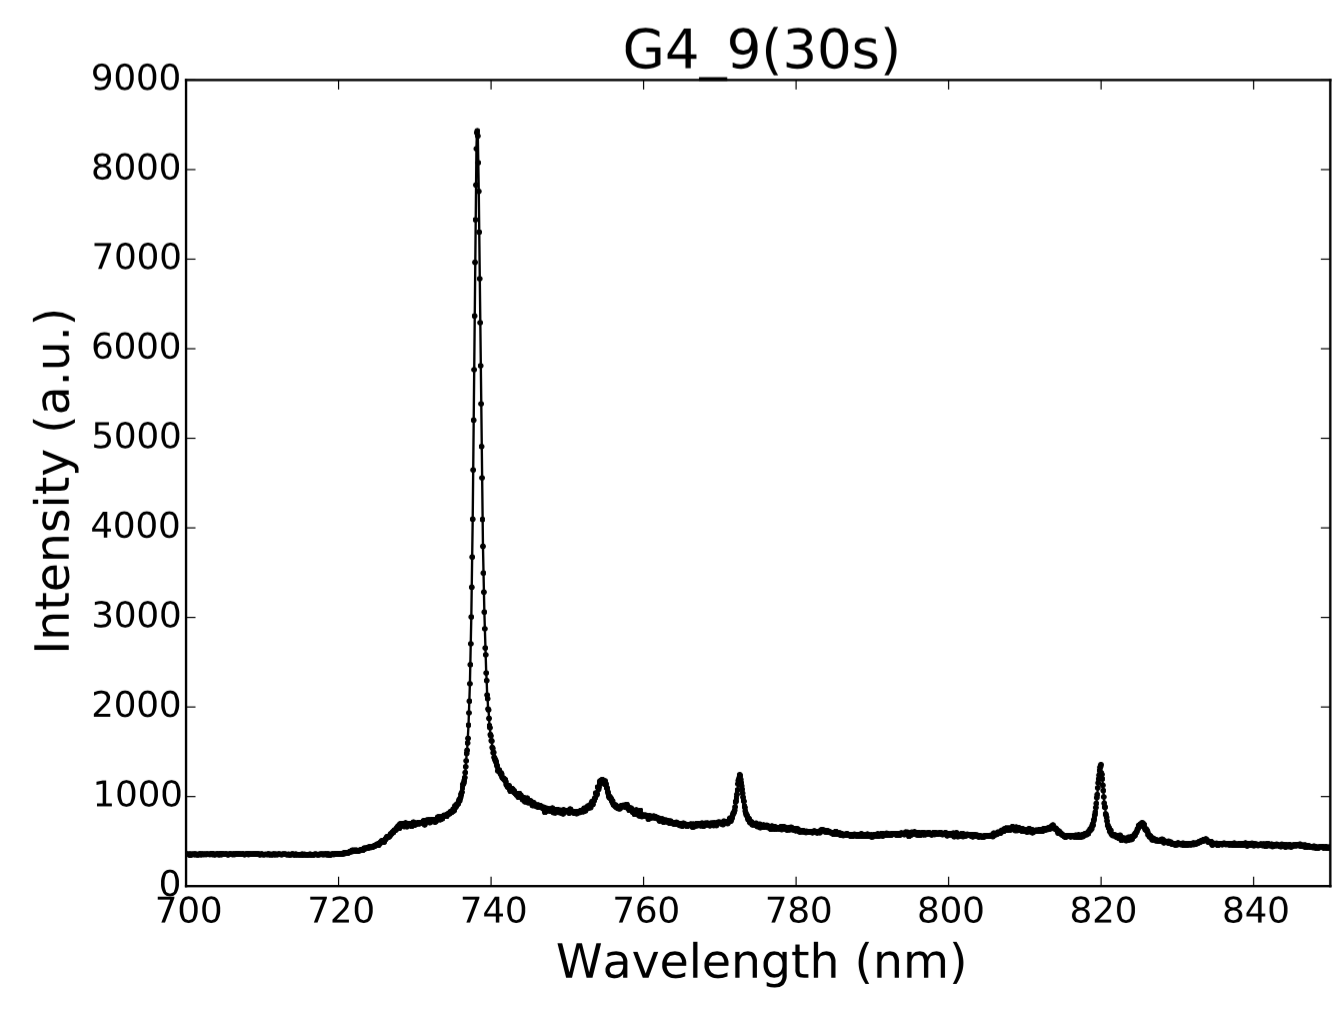
\includegraphics[trim = 0 0 0 0,  clip= true, width = \pairplotwide]{./pics/G4_9_30s.png}}
				\caption{}
				\label{subfig::sideband_group_h}
			\end{subfigure}
			\caption[Side band peaks for \sivs]{Representative spectra of emitters showing single (\subref{subfig::sideband_group_v}) and multiple (\subref{subfig::sideband_group_h}) side band peaks. The former belong to \vl, while the latter are members of \hl.}
			\label{fig::sideband_groups}
		\end{figure}

		Most of the spectra in \vl exhibit a characteristic shape, composed of the \ZPL and one strong sideband peak.
		\SI{70}{\percent} of the \pl spectra with one distinct sideband peak exhibit a shift of the sideband peak from the \ZPL between \SIrange{37}{43}{meV}.
		The range of line shifts for the prominent sideband peak coincides with a well-known feature at \SI{42}{meV}, associated with \sivs \cite{Larkins1971,Sternschulte1994}, but also to a larger number of optically active defects \cite{Sternschulte1994}.
		The occurrence of this \SI{42}{meV} sideband feature for a large number of defects and the absence of isotopic variations \cite{Dietrich2014}, favors an assignment as non-localized lattice vibration.
		We furthermore observe that the dominant sideband peak shifts towards smaller distance from the \ZPL for increasing \ZPL \cwl, i.e.\ increasing strain. \Fref{fig::sideband_fit} presents a linear fit to data for emitters in \vl..
		The low phonon energy of the sideband feature and its shift with strain might arise from a local ``softening'' of the crystal lattice in the vicinity of a defect \cite{Sternschulte1994}.

		\begin{figure}[!htb]
			\centering
			\testbox{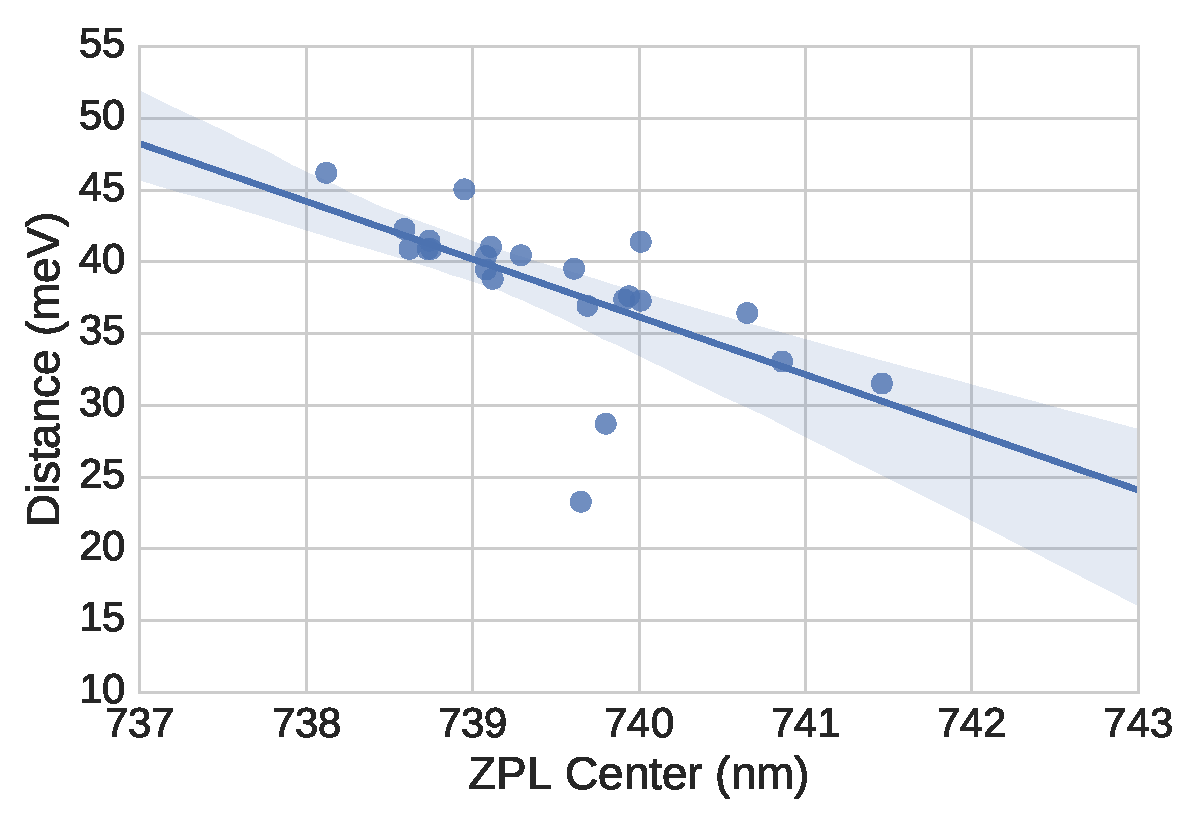
\includegraphics[trim = 0 0 0 0,  clip= true, width = 0.6\linewidth]{./pics/sideband_regression.pdf}}
			\caption[Shift of dominant side band peaks for \sivs]{Shift of dominant sideband peak from the \ZPL in spectra of \sivs (\vl, samples \insituF, \insituS, \insituH) vs. ZPL \cwl. The linear fit shows that the shift decreases with increasing ZPL center wavelength, i.e.\ with increasing strain and exhibits a slope of \SI[separate-uncertainty]{-4\pm1}{\milli\electronvolt\per\nano\meter}. The shaded area is the \SI{95}{\percent} confidence region.}
			\label{fig::sideband_fit}
		\end{figure}

		A recent study \cite{Londero2016} suggests that the \SI{42}{meV} mode, similar to other broad \psb features, originates from a resonance attributed to phonons causing the dynamical Jahn-Teller effect with \sivs \cite{Fu2009}.
		As the Jahn-Teller coupling varies with strain it is also expected that the resonance shifts accordingly.
		\\
		In the spectra of \vl, we do not observe a typical \siv sideband feature at \SI{64}{meV}, attributed to a local vibration of the \si atom, frequently much stronger than the  \SI{42}{meV} sideband peak.
		A possible explanation is, that the lattice mode at \SIrange{37}{43}{meV} is so strong that the local vibrational mode at \SI{64}{meV} cannot be separated from the tail of the lattice mode.
		% \\
		% \todo{beginning new}For further investigations, we plotted the \ZPL  of \vl with multiple peaks.
		% We found that two Lorentzian curves fit the peak best.
		% \Fref{fig::sideband_multfit} shows histograms of the distribution of the \cw and the \lw of the fitted peaks.
		% Keep in mind that two of the peaks sum up to the peak visible as a \ZPL and the third peak is the sideband peak which we attribute to the lattice mode at about \SI{43}{meV}.
		% We found that the \lw of the sideband peak exhibits values up to \SI{20}{nm}.
		% This broad width is an indicator, that the local vibrational mode might indeed be outpowered by the more intense lattice mode.
		% However, it is not very easy to find spectra where the sideband peak is pronounced and isolated enough to make proper statistics.
		% The original \ZPL is split up in two peaks, one with a median \cwl of \SI{738}{nm} (\SI{1680}{\meV}) and a median \lw of \SI{4.5}{nm}  and the other with a median \cwl of \SI{742}{nm} (\SI{1671}{\meV}) and a median \lw of \SI{8}{nm}.
		% It could be that this is an indication for another sideband peak with a shift of \SI{9}{\meV}.
		% \todo{end new}
		% \\
		% \begin{figure}[tp]
		% 	\begin{subfigure}[t]{ 0.49\linewidth}
		% 		\centering
		% 		\testbox{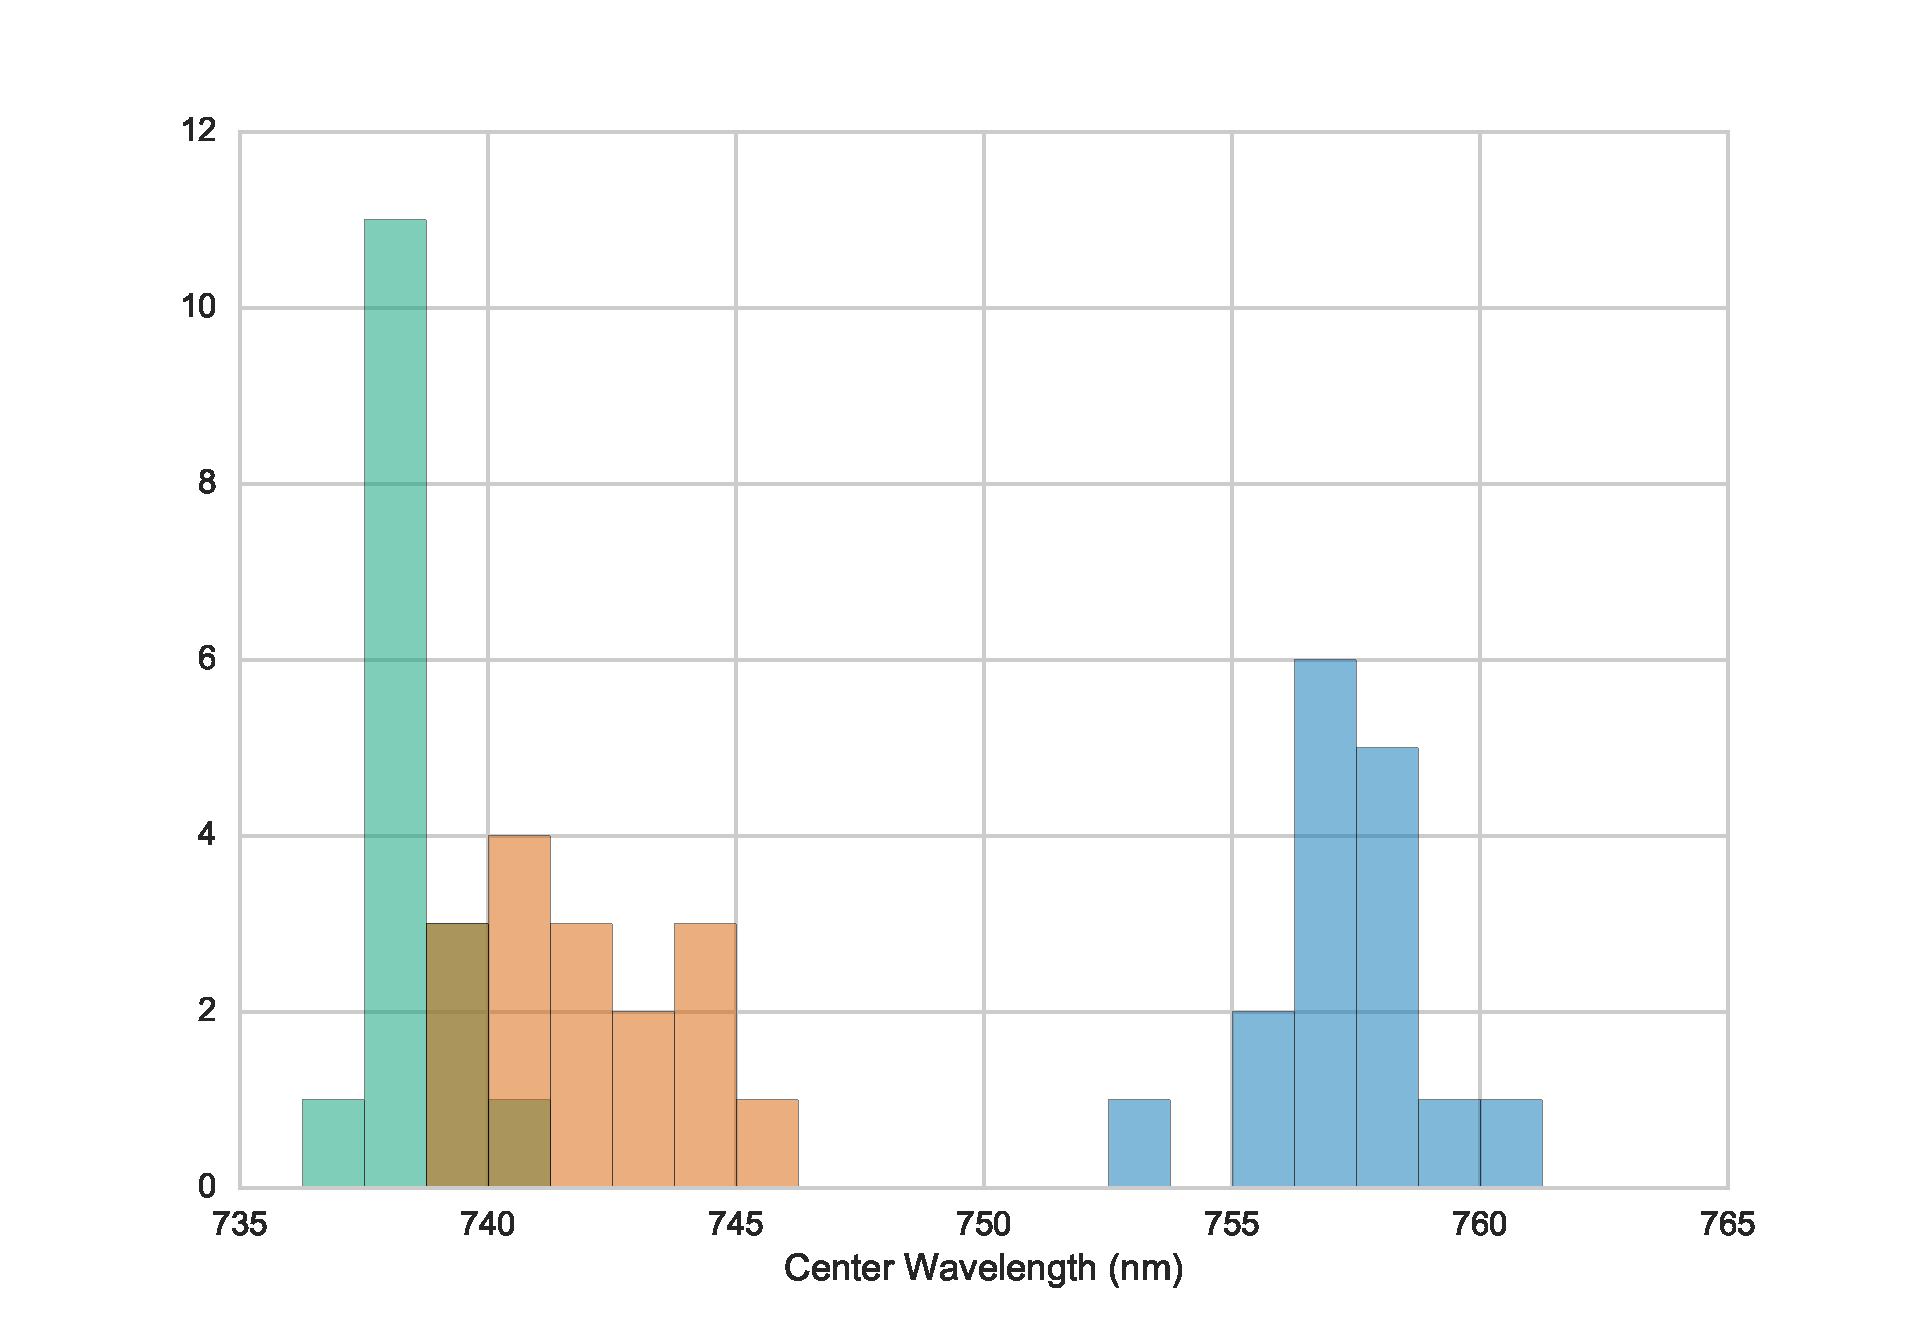
\includegraphics[trim = 0 0 0 0,  clip= true, width = \textwidth]{./pics/histo_multi_sidebands_position25bins.pdf}}
		% 		\caption{}
		% 		\label{subfig::sb_multfit_pos}
		% 	\end{subfigure}
		% 	\hfill
		% 	\begin{subfigure}[t]{ 0.49\linewidth}
		% 		\centering
		% 		\testbox{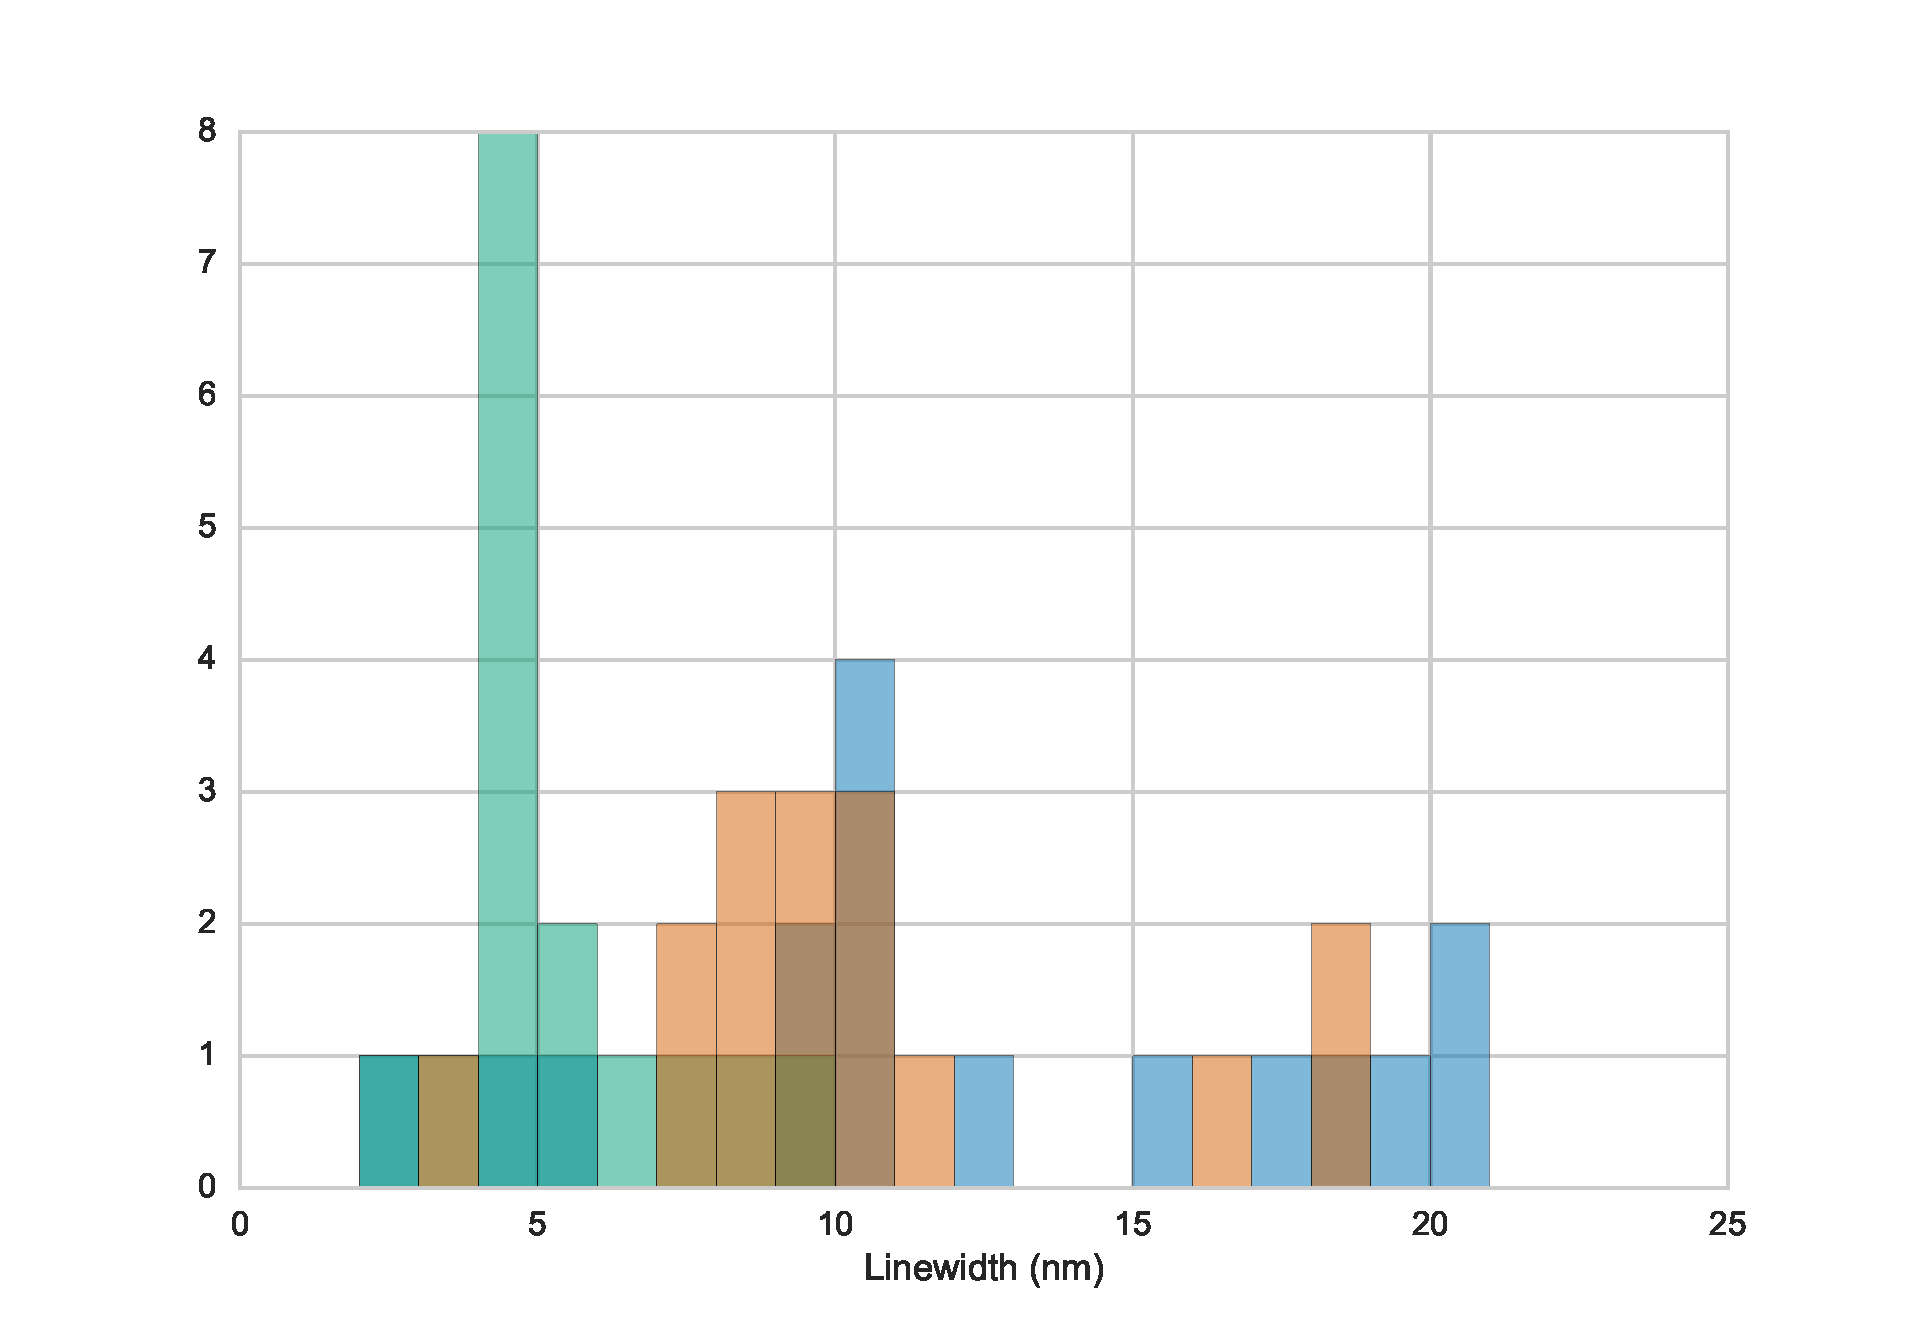
\includegraphics[trim = 0 0 0 0,  clip= true, width = \textwidth]{./pics/histo_multi_sidebands_width_25bins.pdf}}
		% 		\caption{}
		% 		\label{subfig::sb_multfit_width}
		% 	\end{subfigure}
		% 	\caption{}
		% 	\label{fig::sideband_multfit}
		% \end{figure}
		% \\
		In \hl we observe many spectra which exhibit several peaks within the spectral range of our detection range between \SIrange{710}{900}{nm}.
		The challenge arises to unequivocally distinguish between peaks stemming from a phonon sideband and peaks stemming from shifted, less intense \siv \ZPLs.

		Interestingly, we assert a tendency for peaks to accumulate at a shift of around \SIlist{43;64;150;175}{meV}, as shown in \Fref{fig::multiple_sb_peaks}. This pattern in the \psb of \hl is consistent with side band shifts reported in \cite{Sternschulte1994,Zaitsev2000, Neu2011}.

		\begin{figure}[!htb]
			\centering
			\testbox{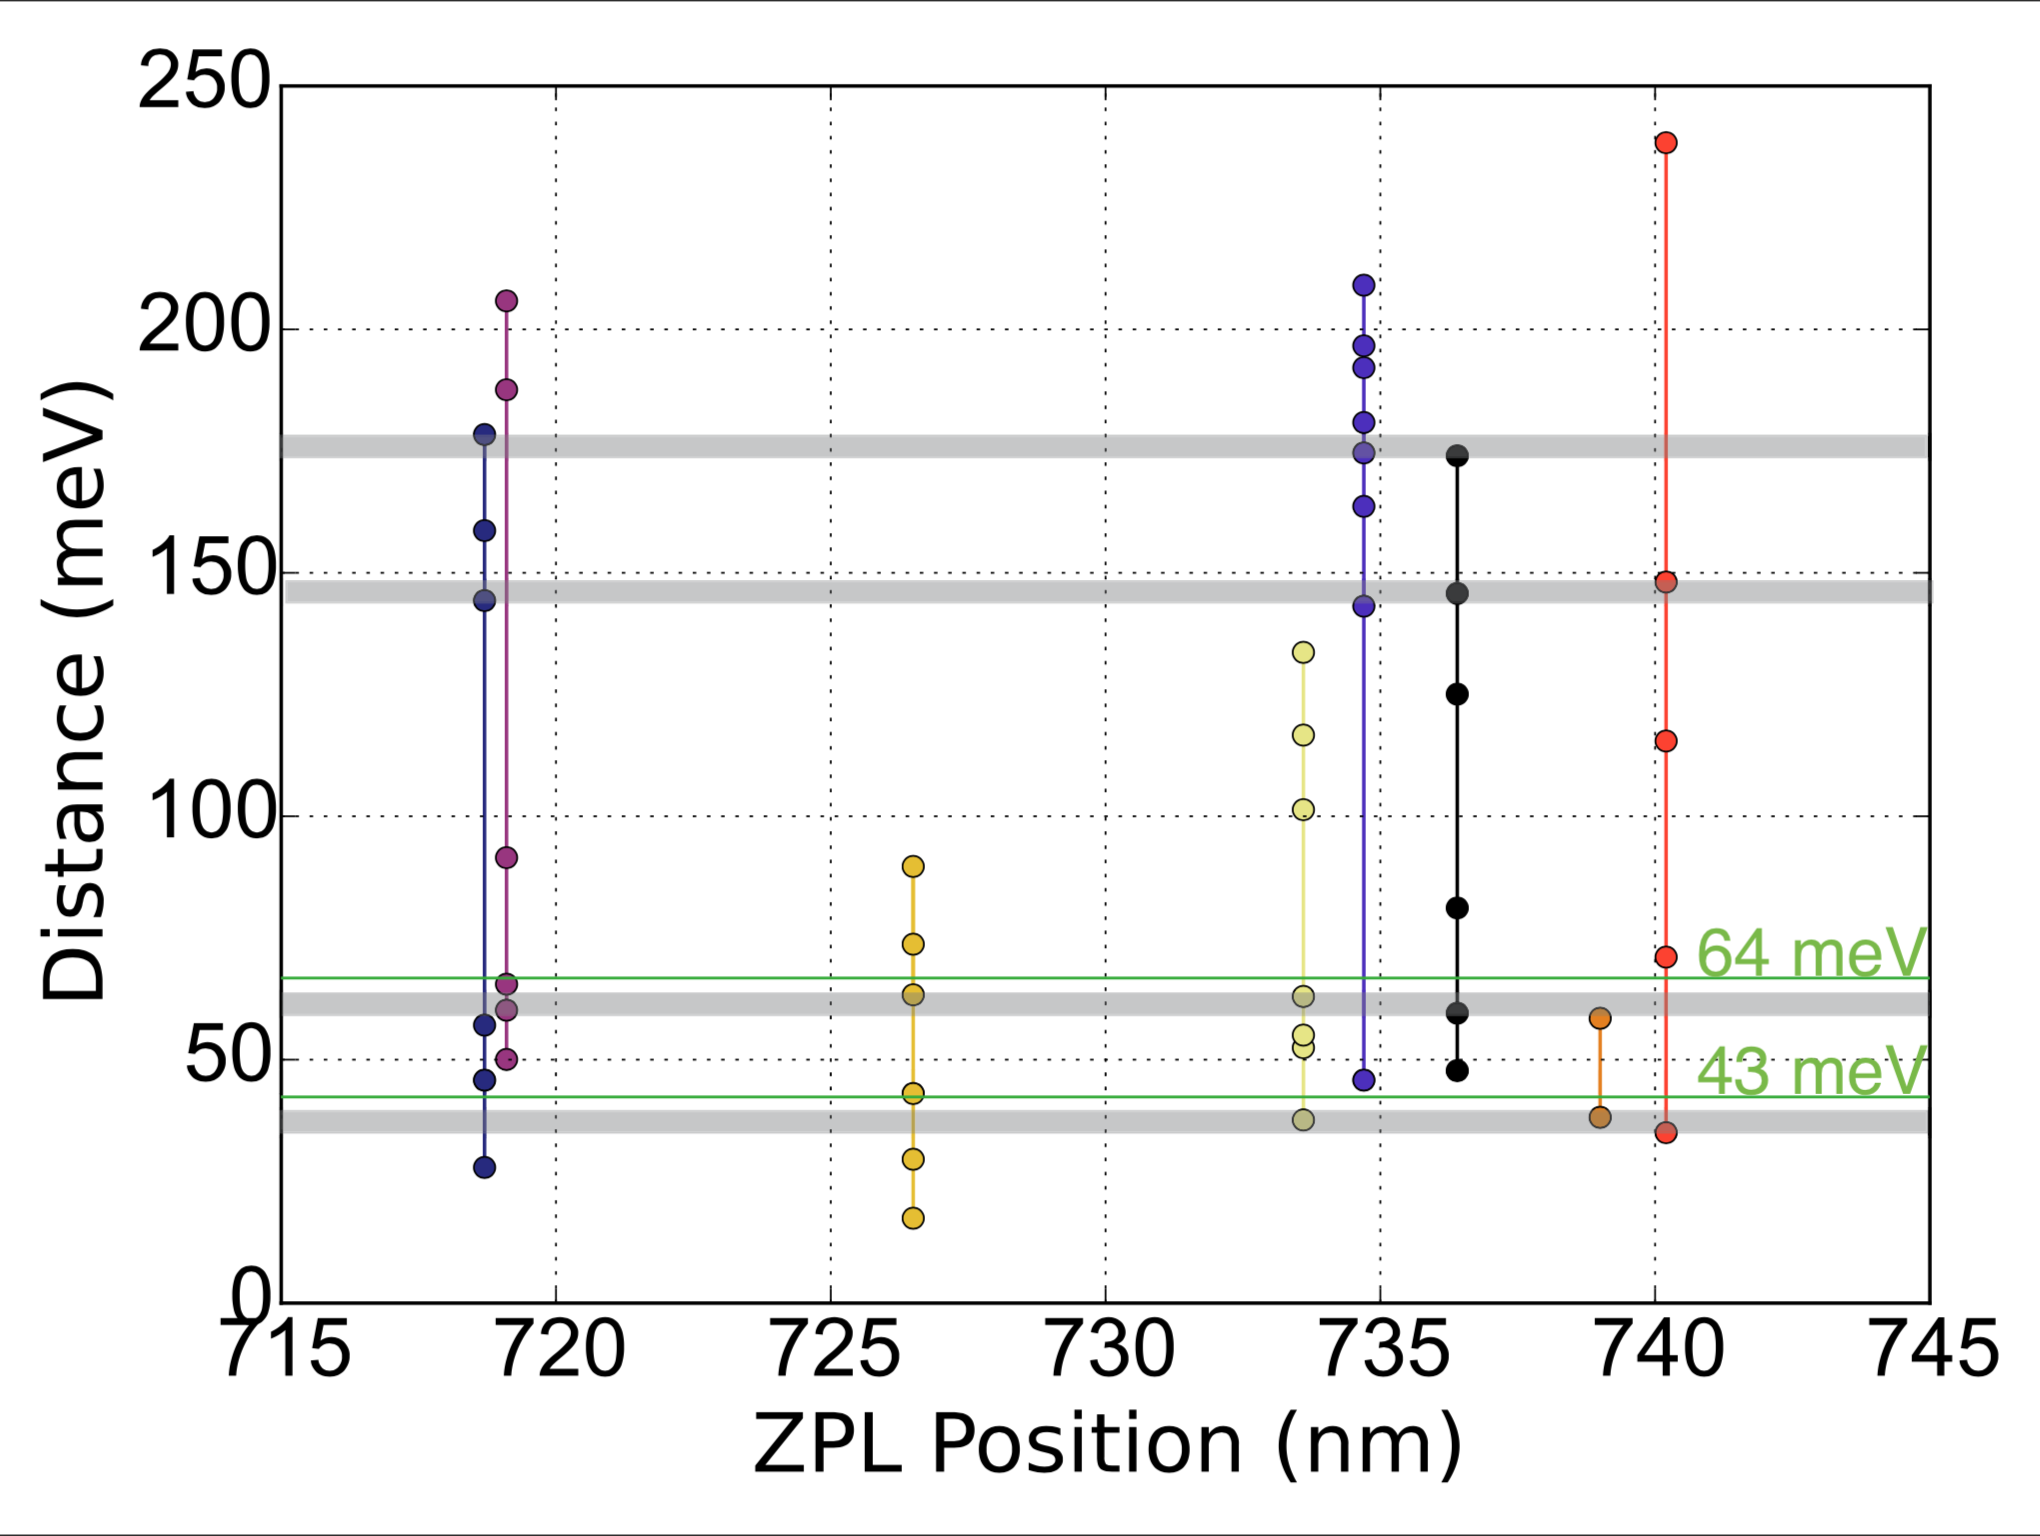
\includegraphics[trim = 0 0 0 0,  clip= true, width = 0.6\linewidth]{./pics/statistics_only_multiple_sb_zpl_vs_distance_5meVbars_modes_edit.png}}
			\caption[Accumulation of sideband peaks]{This plots shows sideband peaks attributed to different \ZPL \cwls, with respect to the sideband peak's shift. The \ZPL \cwl is visualized on the x-axis, the respective sideband peak shifts on the y-axis. Therefore, data points aligned on a vertical line belong to the same spectrum. For better visibility, all data points of one spectrum are colored in the same color. Areas shaded in grey represent an accumulation of sideband shifts. The green lines indicate distances with \SI{43}{meV} and \SI{64}{meV} respectively.}
			\label{fig::multiple_sb_peaks}
		\end{figure}

		The possibility exists, that some these peaks believed to be \psbs are actually shifted \ZPLs stemming from other \sivs. To address this question, we perform \pl measurements at cryogenic temperatures.


		\subsection{Cryostatic Measurements}\label{subsec::cryo}

			\begin{figure}[!htb]
				\begin{subfigure}[t]{ 0.49\linewidth}
					\centering
					\testbox{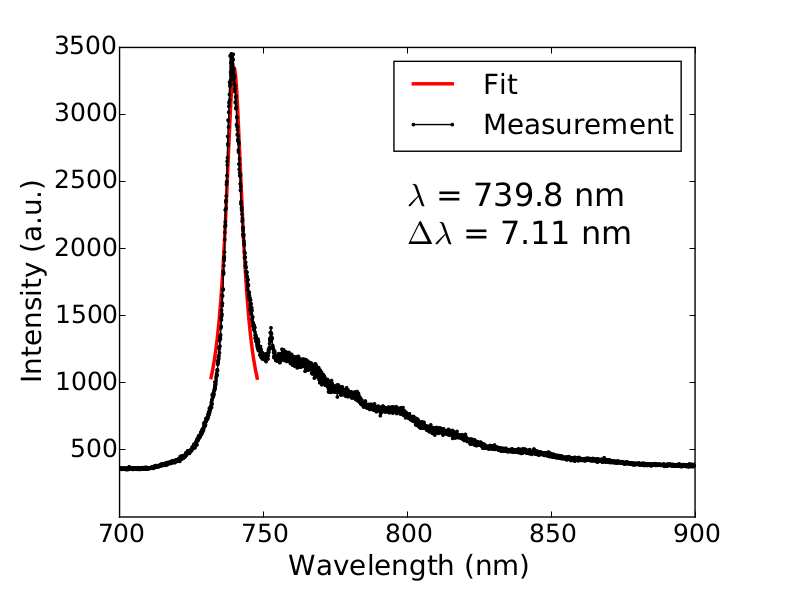
\includegraphics[trim = 0 0 0 0,  clip= true, width = \pairplotwide]{./pics/Ir25Mox_fit_spe_scan_xy-08x11y19_297uW_t180.png}}
					\caption{}
					\label{subfig::roomtep1}
				\end{subfigure}
				\hfill
				\begin{subfigure}[t]{ 0.49\linewidth}
					\centering
					\testbox{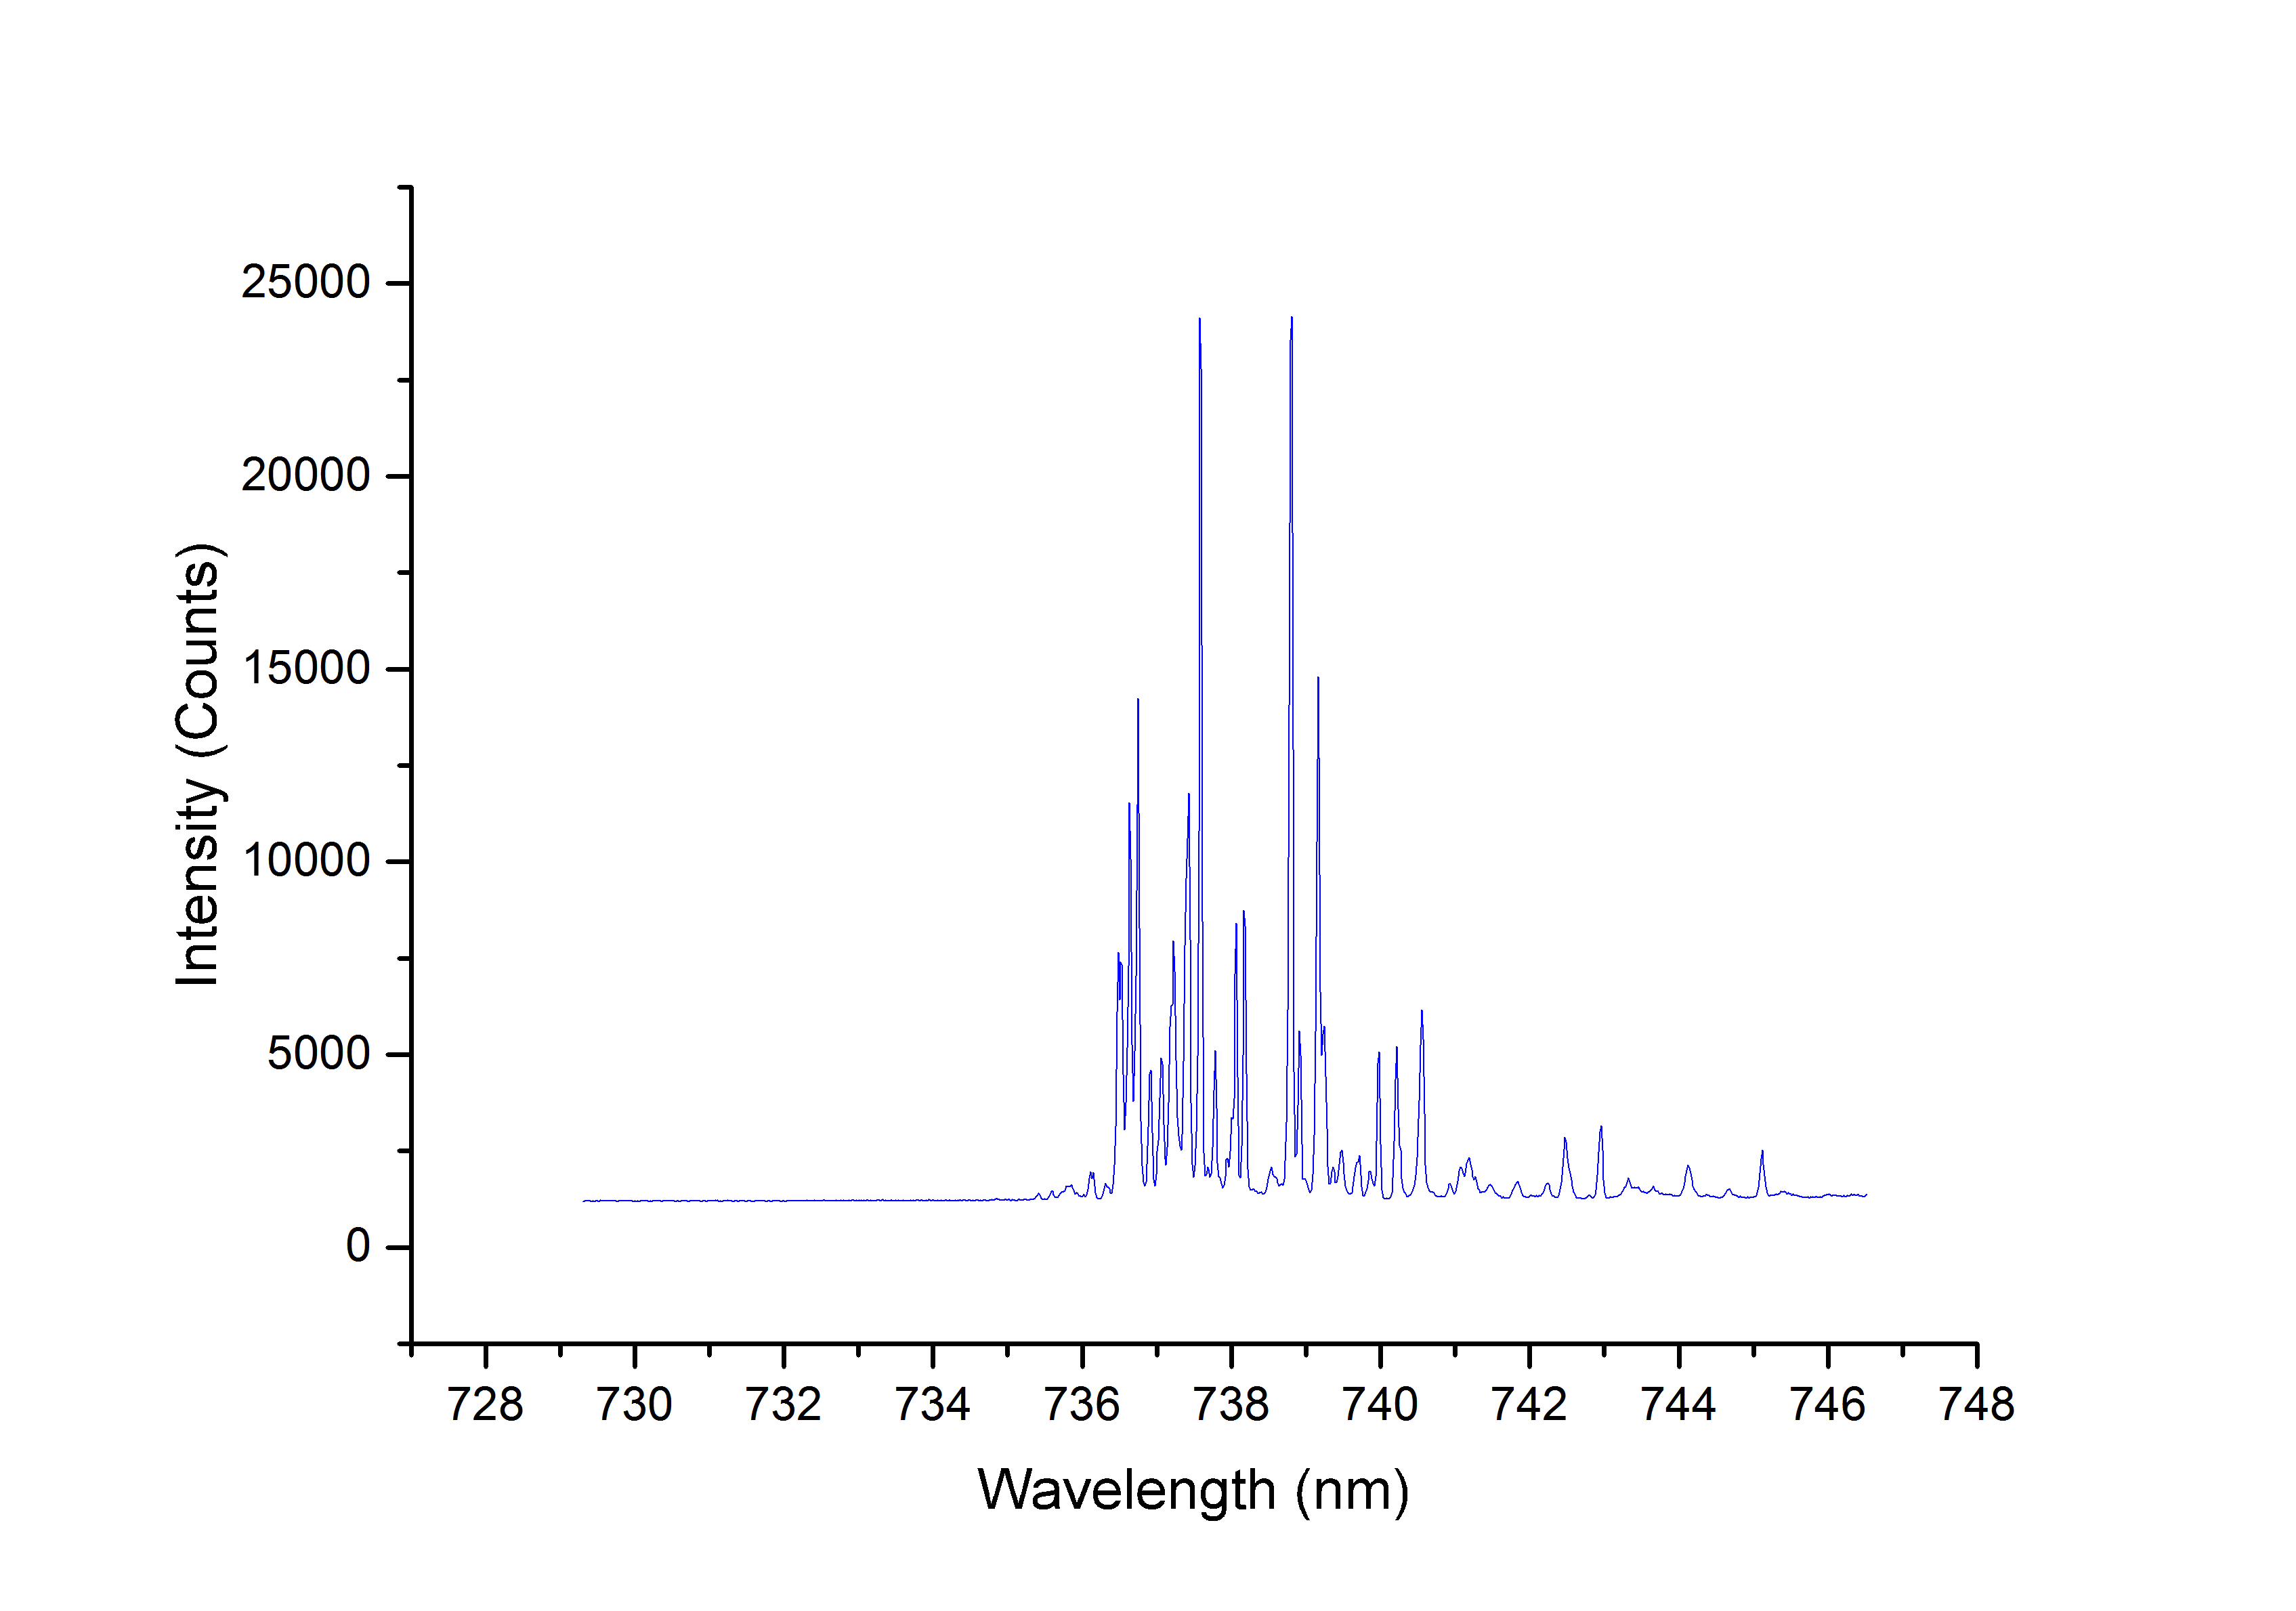
\includegraphics[trim = 0 0 0 0,  clip= true, width = \pairplotwide]{./pics/cryo_Spektrum68_edit.png}}
					\caption{}
					\label{subfig::cryo1}
				\end{subfigure}
				\hfill
				\begin{subfigure}[t]{ 0.49\linewidth}
					\centering
					\testbox{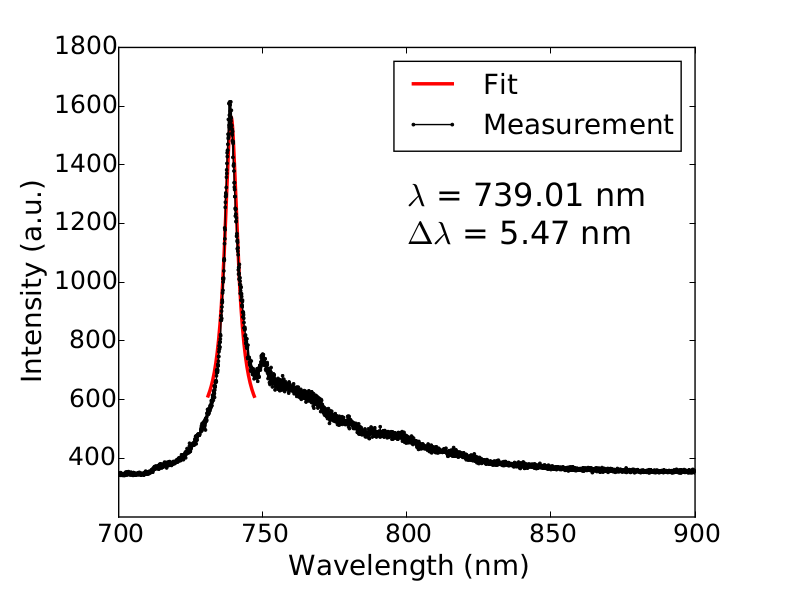
\includegraphics[trim = 0 0 0 0,  clip= true, width = \pairplotwide]{./pics/Ir25M_rt_to_cryo_84_fit_spe_scan_xy-35x10y12_300uW_t120.png}}
					\caption{}
					\label{subfig::roomtep2}
				\end{subfigure}
				\hfill
				\begin{subfigure}[t]{ 0.49\linewidth}
					\centering
					\testbox{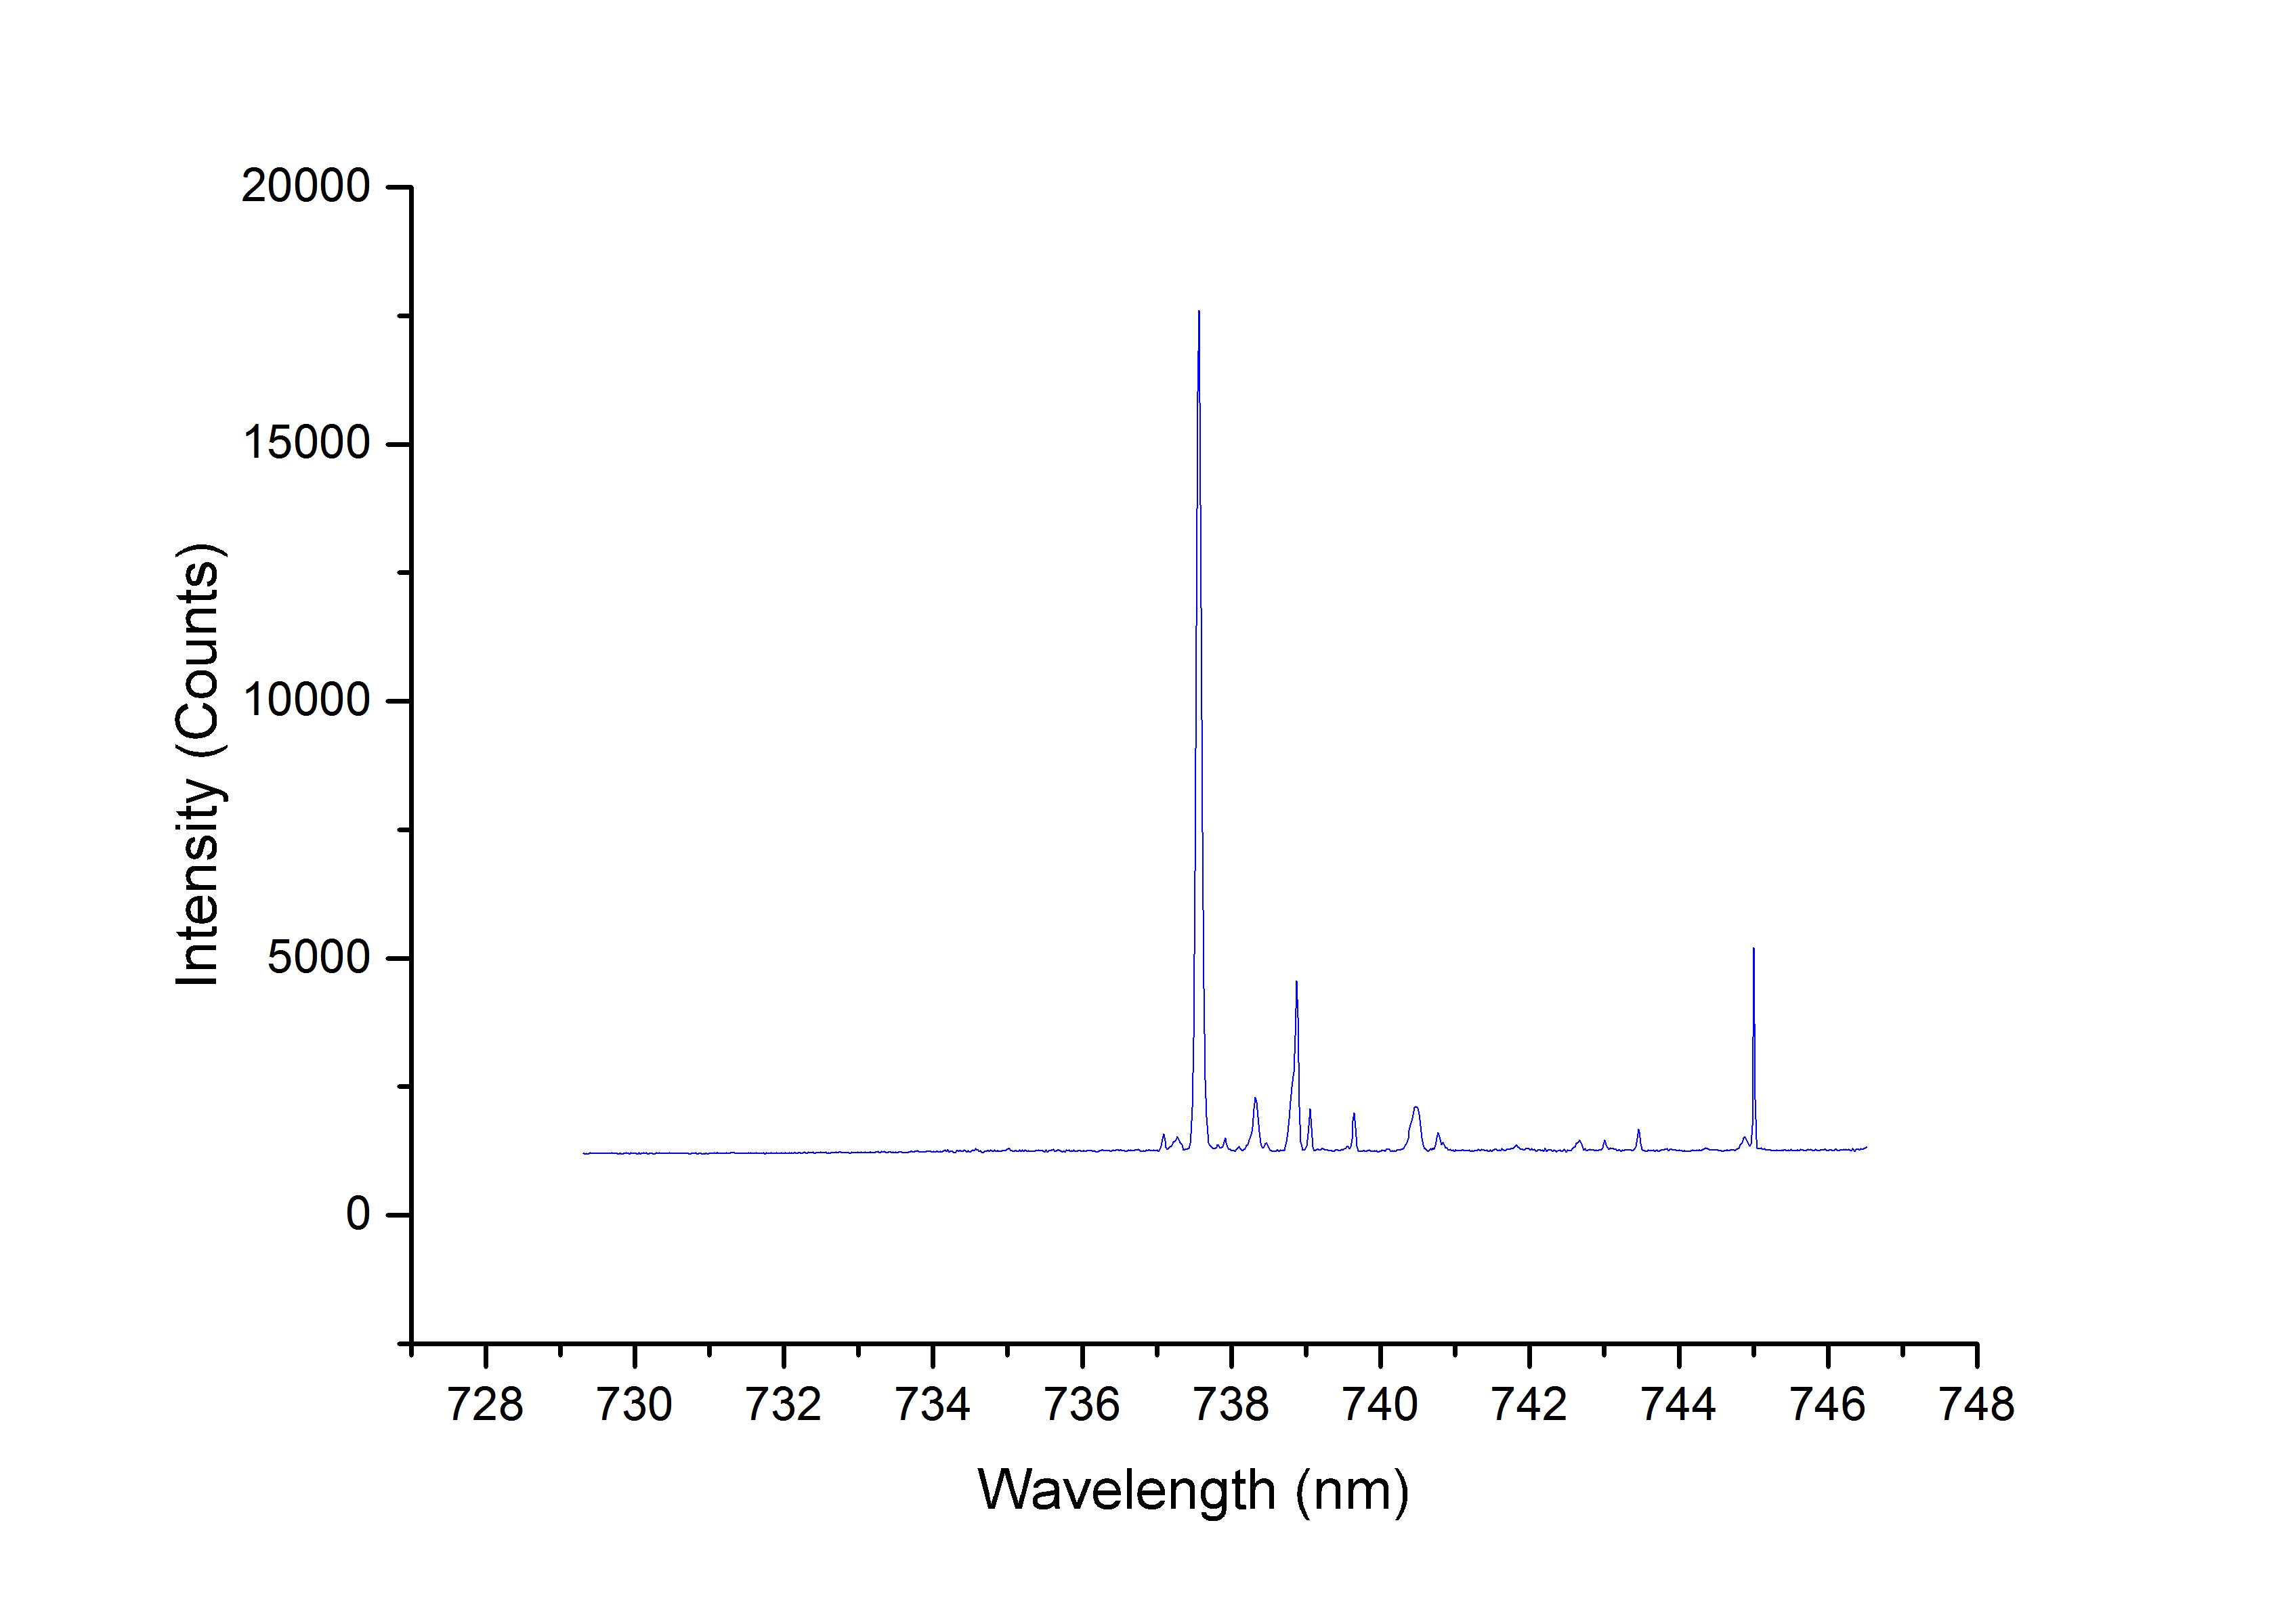
\includegraphics[trim = 0 0 0 0,  clip= true, width = \pairplotwide]{./pics/cryo_Spektrum84_edit.png}}
					\caption{}
					\label{subfig::cryo2}
				\end{subfigure}
				\caption[Spectra of \nds at cryogenic temperatures]{Comparison of spectra taken at room-temperature (l.h.s) and at cryogenic temperatures (r.h.s). At low temperatures a multitude of lines is revealed indicating several \sivs embedded in a strained lattice neighborhood.}
				\label{fig::rt_vs_cryo}
			\end{figure}

			At cryogenic temperatures \psb contributions vanish, allowing a focused investigation of \zpls.
			In particular, for \sivs a four-way splitting of the \zpl is expected, see \Fref{ch::introduction}.
			To conduct low-temperature measurements, we used a confocal setup similar to the one described in \Fref{ch::pl_setup}.
			It differs merely by the fact that the sample is efficiently cooled to \SI{4}{\kelvin} using a cryostat.
			\\
			In \Fref{fig::rt_vs_cryo} measurements of two individual \nds are shown, both situated on sample \insituSo.
			\Fref{subfig::cryo1} and \Fref{subfig::cryo2} show spectra recorded at cryogenic temperatures while \Fref{subfig::roomtep1} and \Fref{subfig::roomtep2} show spectra recorded at room temperature for comparison.
			Instead of the four-fold degeneracy expected for \sivs in low-strain diamond, the cryogenic measurements indicate a multitude of various lines.
			The observation is best explained by the presence of several \sivs which are subject to varying levels of strain in their local lattice neighborhood.
			Given the fact that \zpls are found spread over a significant range of \wls, a non-negligible impact of lattice strain on \siv luminescence is revealed.

	%!TEX root = ../../../main.tex

	\section{Photon correlation measurements} \label{subsec::g2}

		The investigated \sivs exhibit count rates of a few thousand to a few \num{100000} counts per second (\SI{}{\cps}).
		We carried out measurements of the photon statistics and found that about \SI{3}{\percent} of luminescent \nds contain single color centers.
		These measurements show, that the probability of finding a single emitter does not correlate in any way with the \cwl or the \lw of the ZPL.
		We found several single \sivs with an anti-bunching dip down to about \num{0.2} and attribute the residual \gtz value to background fluorescence from the diamond host.
		For the utilized \nds a background measurement without simultaneously measuring \siv \pl is infeasible, because the laser spot size is bigger than the \nd, i.e.\ the \siv will always be excited when the \nd is illuminated.
		Therefore, the background is estimated from the sideband of \siv spectra.
		The measured lifetimes of the single \sivs are in the range of about \SIrange{1}{9}{\ns}, which is of the same order as previous research suggests \cite{Sipahigil2014,Sternschulte1994}.

		\Fref{fig::g2} shows the \gt functions of one emitter of \hl and one emitter of \vl.
		The former emitter's spectrum is shown in \Fref{subfig::erlangen_spectrum}, and denoted \emhtwo. The latter is the same as \embroad introduced in \Fref{sec::spectra}.

		\begin{figure}[!htb]
			\begin{subfigure}[tp]{ 0.49\linewidth}
				\centering
				\testbox{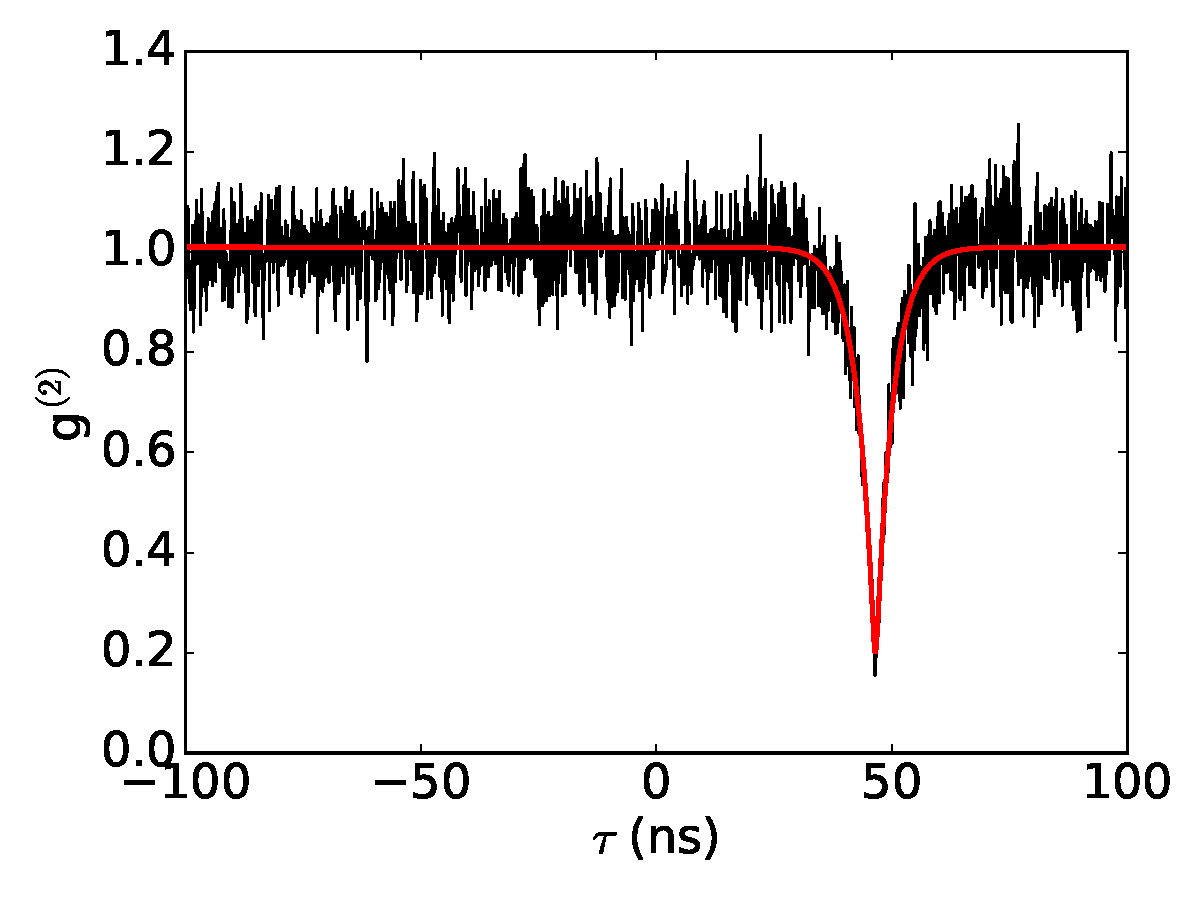
\includegraphics[trim = 0 0 0 0,  clip= true, width = \pairplotwide]{./pics/siv_sarah_g2_90k_2_notitle_original_fit.pdf}}
				\caption{}\label{subfig::g2_a}
			\end{subfigure}
			\hfill
			\begin{subfigure}[tp]{ 0.49\linewidth}
				\centering
				\testbox{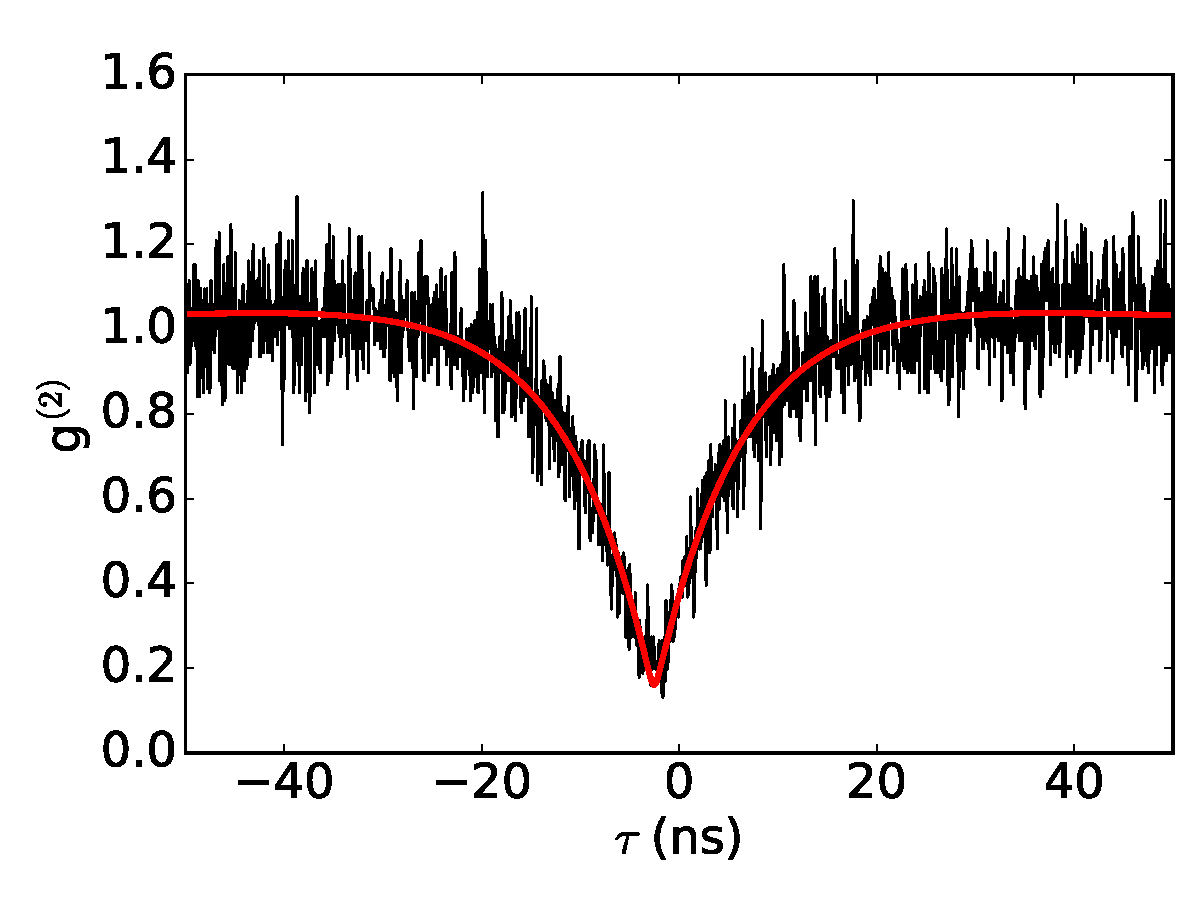
\includegraphics[trim = 0 0 0 0,  clip= true, width = \pairplotwide]{./pics/Ir8_g2_scan_xy-05_200uW_fit.pdf}}
				\caption{}\label{subfig::g2_b}
			\end{subfigure}
			\caption[Intensity autocorrelation measurements for \hl and \vl]{(a) Intensity autocorrelation function of an emitter in \hl. (b) Intensity autocorrelation function of \embroad at an excitation power of \SIlist{200}{\micro\W}. Saturation power is \SI{1}{mW}.}
			\label{fig::g2}
		\end{figure}

		\begin{figure}[!htb]
			\begin{subfigure}[t]{ 0.49\linewidth}
				\centering
				\testbox{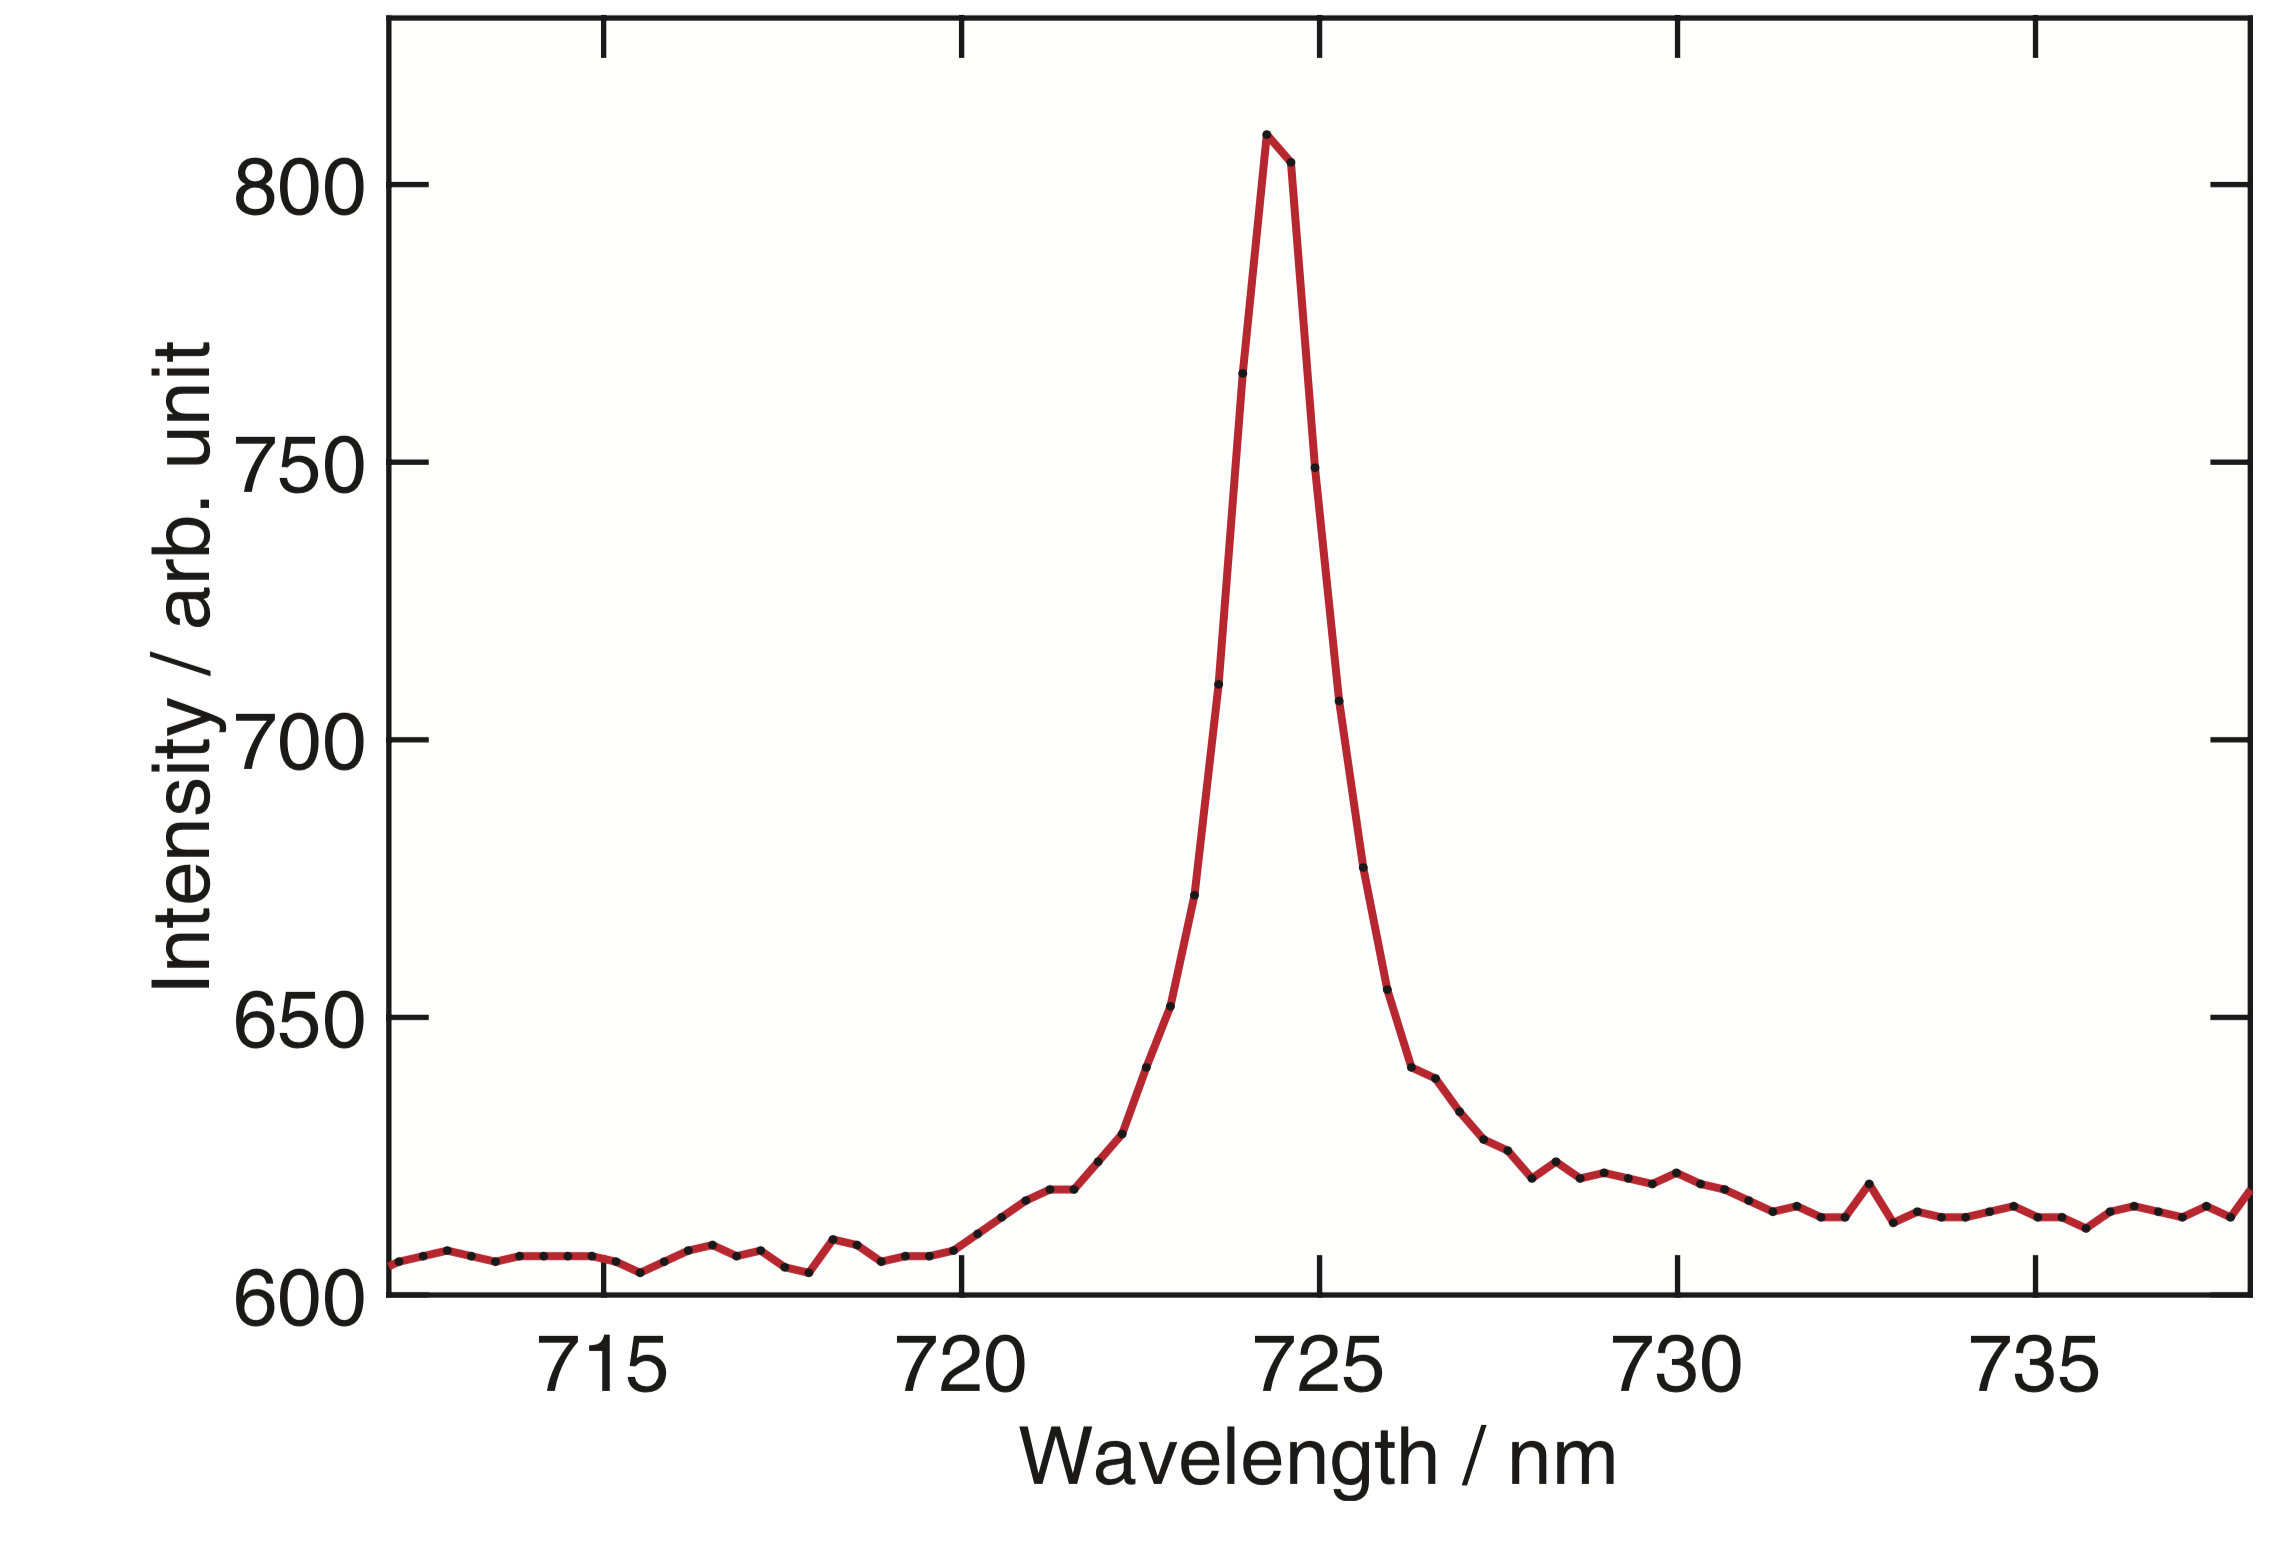
\includegraphics[trim = 0 0 0 0,  clip= true, width = \pairplotwide]{./pics/spectrum_erlangen_publication.png}}
				\caption{}
				\label{subfig::erlangen_spectrum}
			\end{subfigure}
			\hfill
			\begin{subfigure}[t]{ 0.49\linewidth}
				\centering
				\testbox{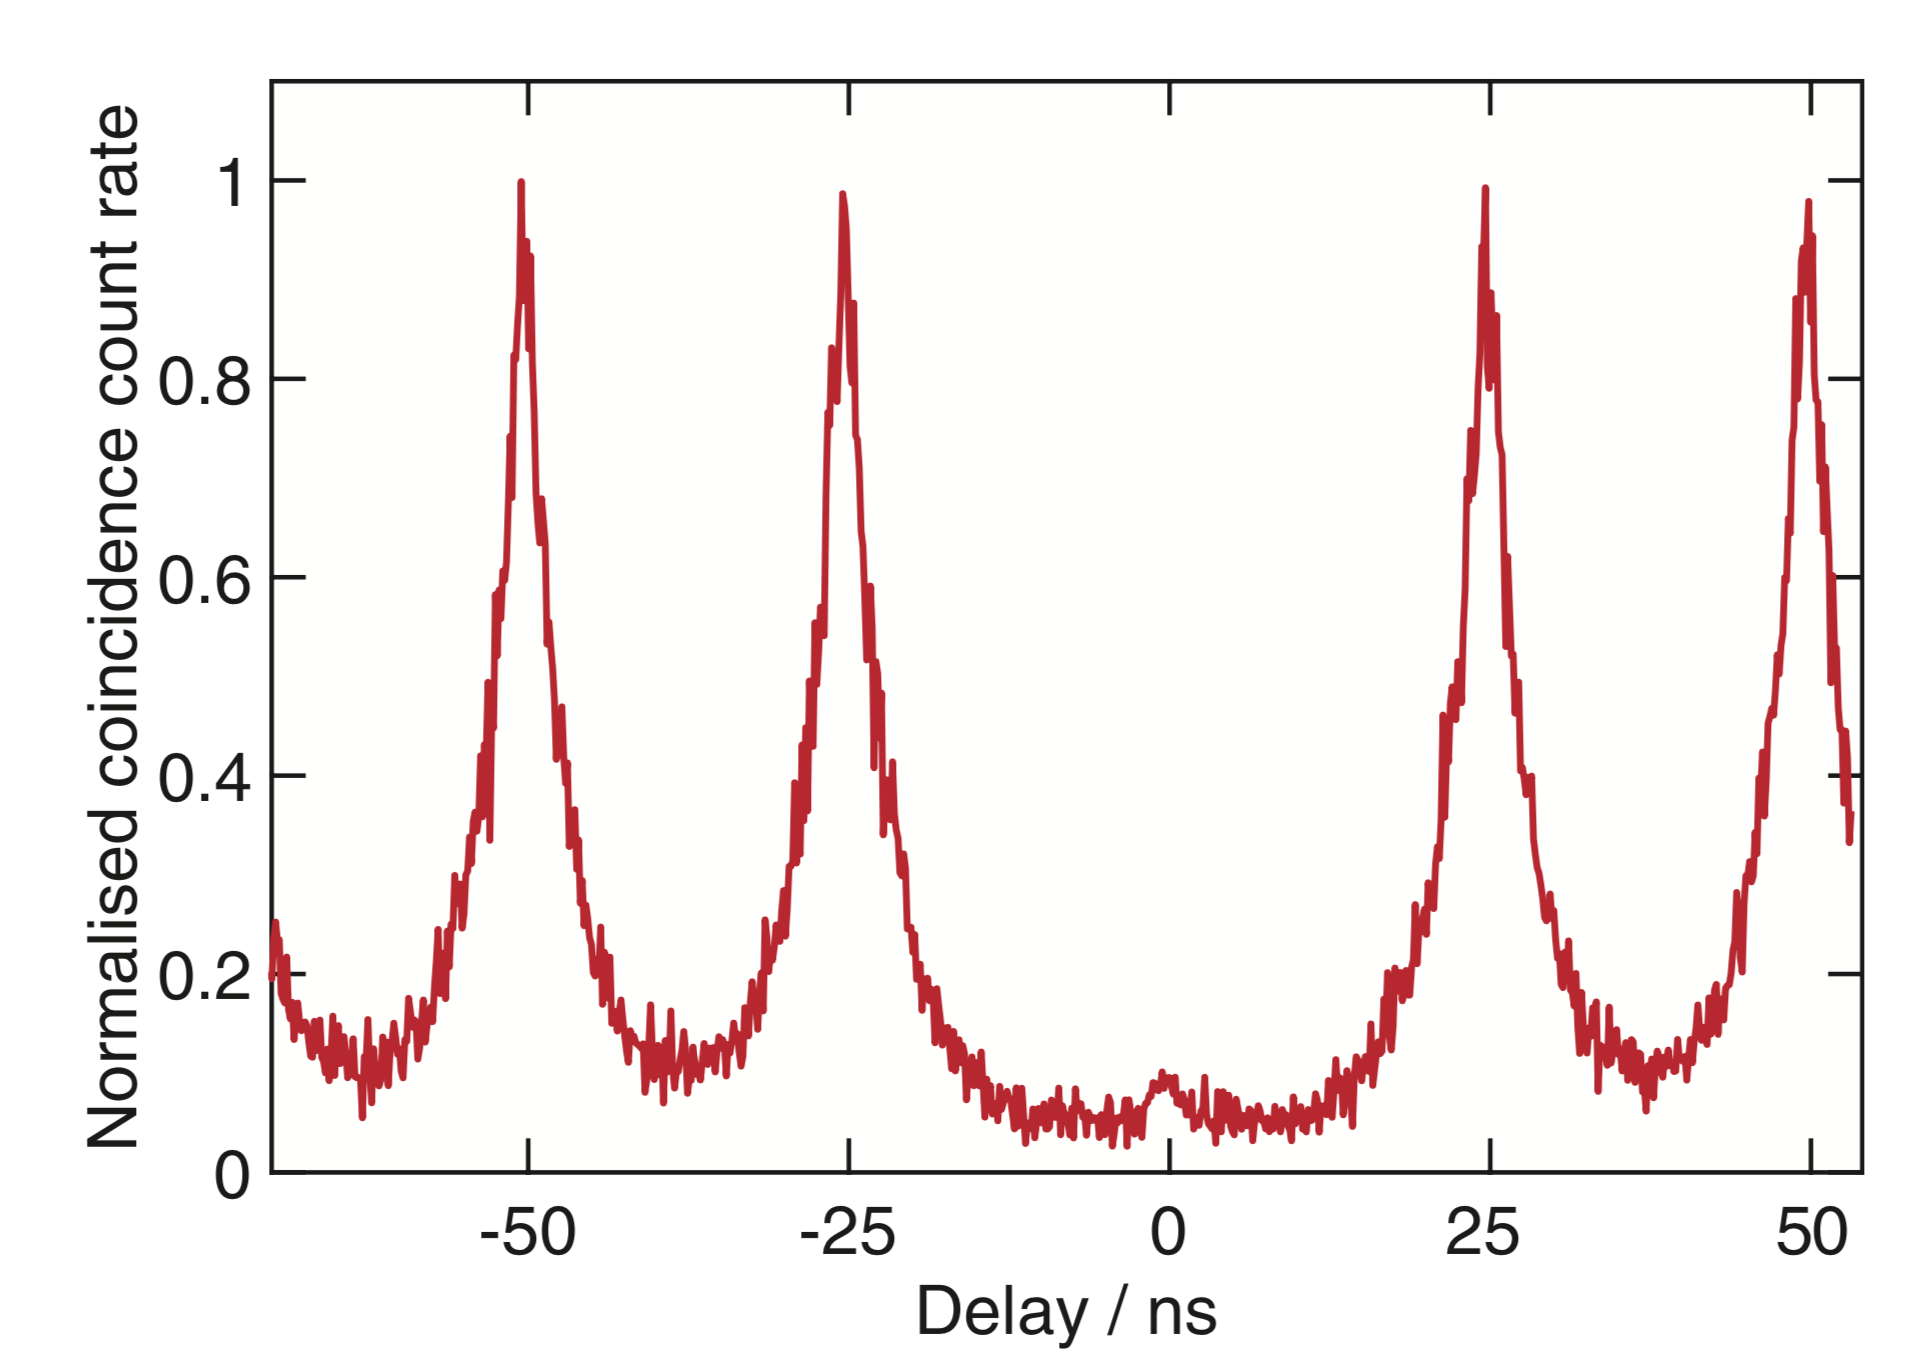
\includegraphics[trim = 0 0 0 0,  clip= true, width = \pairplotwide]{./pics/g2_erlangen_publication.png}}
				\caption{}
				\label{subfig::erlangen_lifetime}
			\end{subfigure}
			\caption[Spectrum and pulsed \gtf of an emitter]{(a) Spectrum of emitter \emhtwo. The \cwl amounts to \SI{724}{nm} and the \lw to \SI{2.0}{nm}. (b) Pulsed \gtf of the same emitter. \gtz amounts to \num{0.2}. Figures reproduced from \cite{Vaigu2017}.}
			\label{fig::erlangen_spectrum_lifetime}
		\end{figure}

		\Fref{subfig::g2_a} shows the photon correlation function of \emhtwo under \cw excitation.
		The shift of the dip to $\tau=\SI{50}{ns}$ originates from a path length difference of the two detection paths in the \HBT setup.
		The \gtz value of the fit is \num{0.20}.
		\\
		We also performed measurements with a pulsed laser, which is a prerequisite for a direct link between the high photon flux levels of the classical regime and low photon flux levels in the quantum world \cite{Vaigu2017,SiquteProject}, as mentioned in \Fref{ch::introduction}.
		The pulsed second-order correlation at zero delay \gtz are calculated by integrating photon counts in the zero-time-delay peak and dividing by the average of the adjacent peaks.
		\\
		The excited state lifetime of the emitter was determined to be \SI[separate-uncertainty]{3.8\pm0.1}{ns}, see \Fref{fig::lifetime}.
		For this, the emitter is excited by a pulsed laser (PiL069XSM from Advanced Laser Diode Systems A.L.S. GmbH) produces short optical pulses of less than \SI{50}{\ps} at a maximum repetition rate of \SI{80}{\mega\hertz} and a wavelength of \SI{685}{\nm} \cite{Vaigu2017}. 
		The measured time intervals between the optical pulse and the detected \fl yields the exponentially decaying lifetime of the excited state.
		The lifetime of the emitter is the time interval after which the number of $N_0$ excited emitters decreases to $N_0/e$.
		
		\begin{figure}[!htb]
			\centering
			\testbox{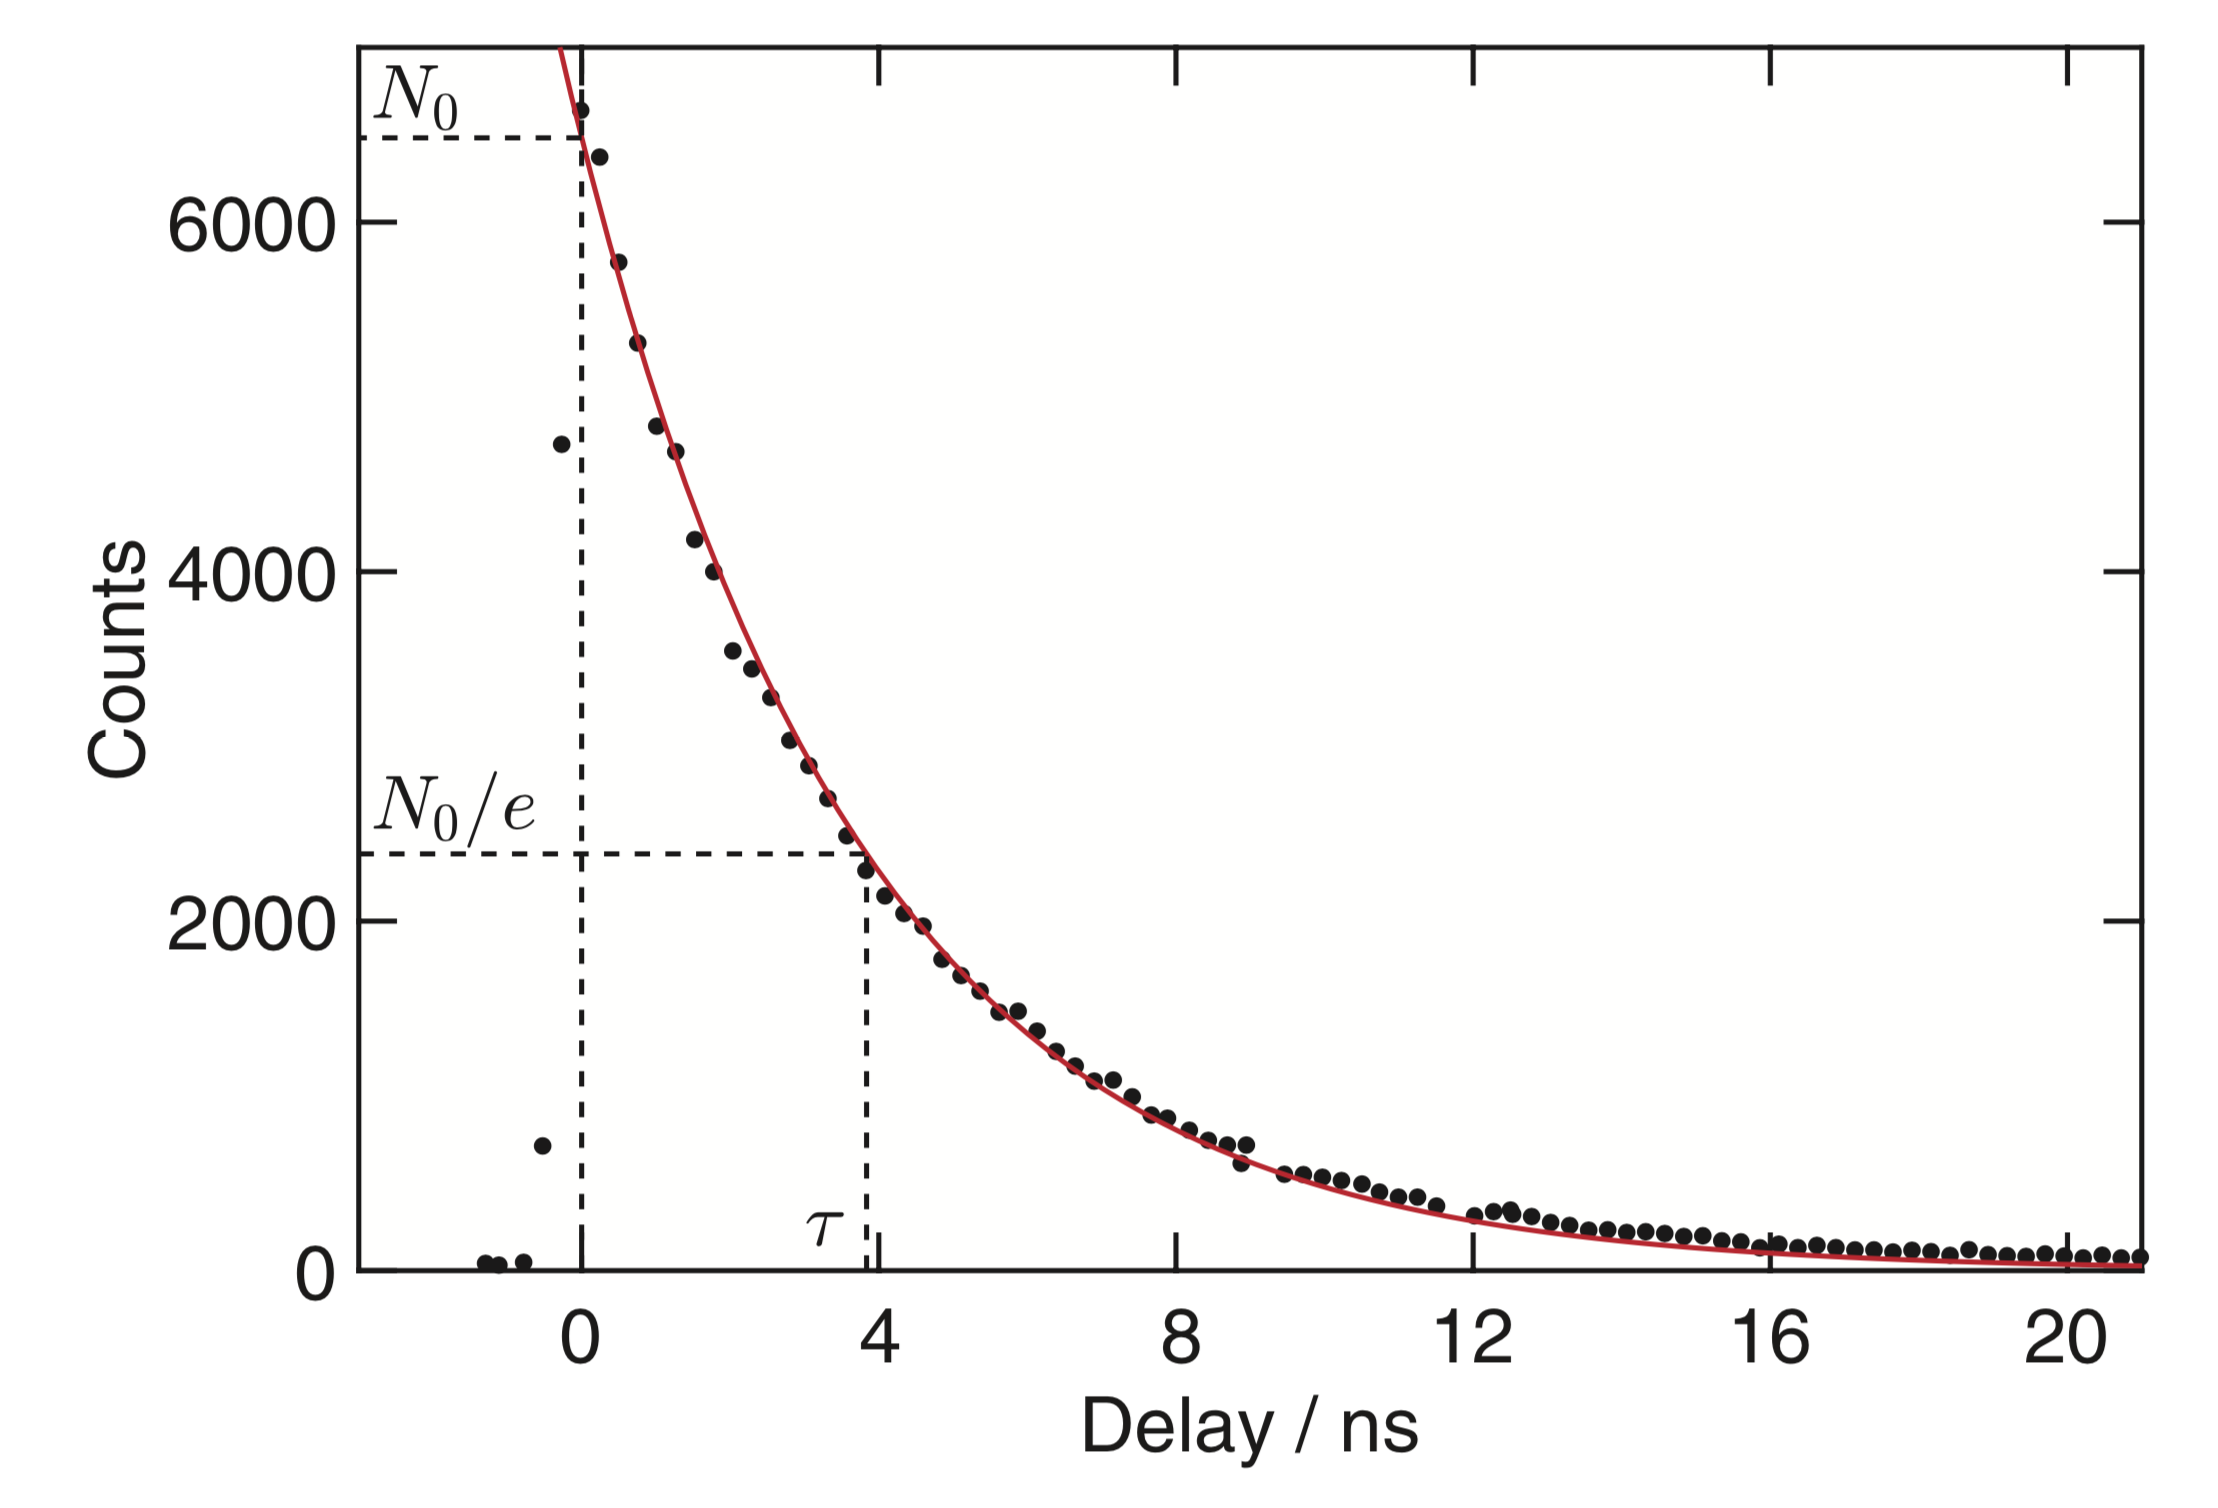
\includegraphics[trim = 0 0 0 0,  clip= true, width = 0.6\linewidth]{./pics/lifetime_erlangen_publication.png}}
			\caption[Lifetime measurement of an emitter]{Lifetime measurement of emitter \emhtwo. The lifetime of the emitter is the time interval after which the number of $N_0$ excited emitters decreases to $N_0/e$. Figure reproduced from \cite{Vaigu2017}.}
			\label{fig::lifetime}
		\end{figure}

		
		\begin{figure}[!htb]
			\centering
			\testbox{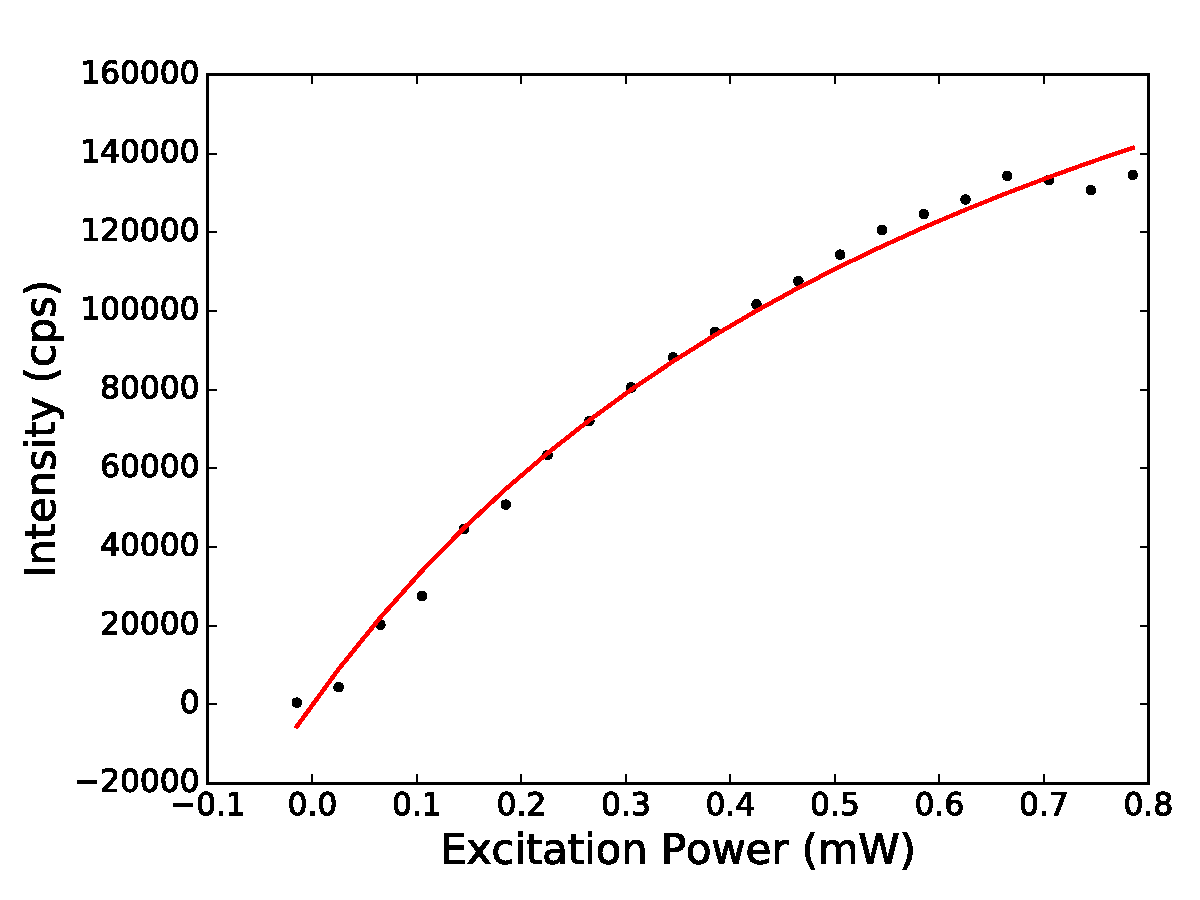
\includegraphics[trim = 0 0 0 0,  clip= true, width = 0.6\linewidth]{./pics/Ir8_sat_scan_xy-05_fit_notitle.pdf}}
			\caption[Saturation measurement of an emitter]{Saturation measurement of emitter \embroad.}
			\label{fig::sat_Ir8}
		\end{figure}

		An important characteristic of \spss is their photon count rate at saturation. The count rate $I(P)$ as a function of the excitation power $P$ is given by
		% 
		\begin{equation}
			I(P) = I_{\infty} \frac{P}{P + P_{sat}} + c_b P.
		\end{equation}

		Here $I_{\infty}$ refers to the maximal photon count rate, while the saturation power is denoted by $P_{sat}$. These two quantities are parameters determined by fitting count rates $I(P)$ measured at different excitation powers $P$. The added term $c_b P$ takes into account the linear increase of background fluorescence from the diamond host material at higher excitation powers. When background effects are negligible, this term can be omitted.

		\Fref{fig::sat_Ir8} depicts the saturation curve of \embroad.
		The saturation count-rate amounts to \SI[separate-uncertainty]{340\pm20}{cps} at a saturation power of \SI[separate-uncertainty]{1.0\pm0.1}{mW}.
		\Fref{subfig::g2_b} shows the \gt function of \embroad at an excitation power of \SI{200}{\micro\W}, which is \SI{20}{\percent} of the emitter's saturation power $P_{sat}=\SI[separate-uncertainty]{1.0\pm0.1}{mW}$.
		The \gtz value yields \num{0.16}.
		It is a \gt measurement representative of single \sivs.
		It is well below \num{0.5}, indicating single photon emission.
		The non-vanishing \gtz value is caused by background fluorescence of the diamond.
		The lifetime of the excited state of this emitter is \SI[separate-uncertainty]{9.2\pm0.2}{ns}.
		It is the highest excited state lifetime we measured within this work.
		\\
		Several \nd \pl spectra contain multiple narrow distinct peaks at different \wls.
		This circumstance is attributed to \nds containing more than one \siv, each of which is subject to a different \ZPL \wl shift.
		We choose narrow bandpass filters to perform independent measurements of each individual peaks of such a spectrum.
		As a result it is possible to measure \gtz values below \num{0.5} for each of these narrow peaks.
		Hence the individual peaks are identified as single emitters with a different ZPL \cwl.
		\\
		We do not see a systematic difference regarding the photon autocorrelation functions of \hl and \vl, both reach similar \gtz values.
		Also, the timescales of the excited state lifetimes coincide.

	%!TEX root = ../../../main.tex

	\section{Photostability} \label{subsec::photostab}

		As mentioned in the previous section, the single photon count rates observed from the investigated \sivs varies strongly between a few thousand to a few \SI{100000}{cps}.
		To further investigate the count rate, the luminescence time trajectory of the emitters which exhibit a dip at \gtz is evaluated.
		It is found that some of the observed emitters exhibit fluorescence intermittence, also called blinking. \Fref{fig::blink} illustrate the effect.
		Blinking is attributed to temporal ionization of the color center during optical excitation, forming an optically inactive charge state \cite{Jantzen2016,Neu2012a,Gali2013}.
		Therefore the emitters change between states of higher and lower emission, i.e.\ brighter and darker states, called blinking levels.

		\begin{figure}[!htb]
			\begin{subfigure}[tp]{ 0.49\linewidth}
				\centering
				\testbox{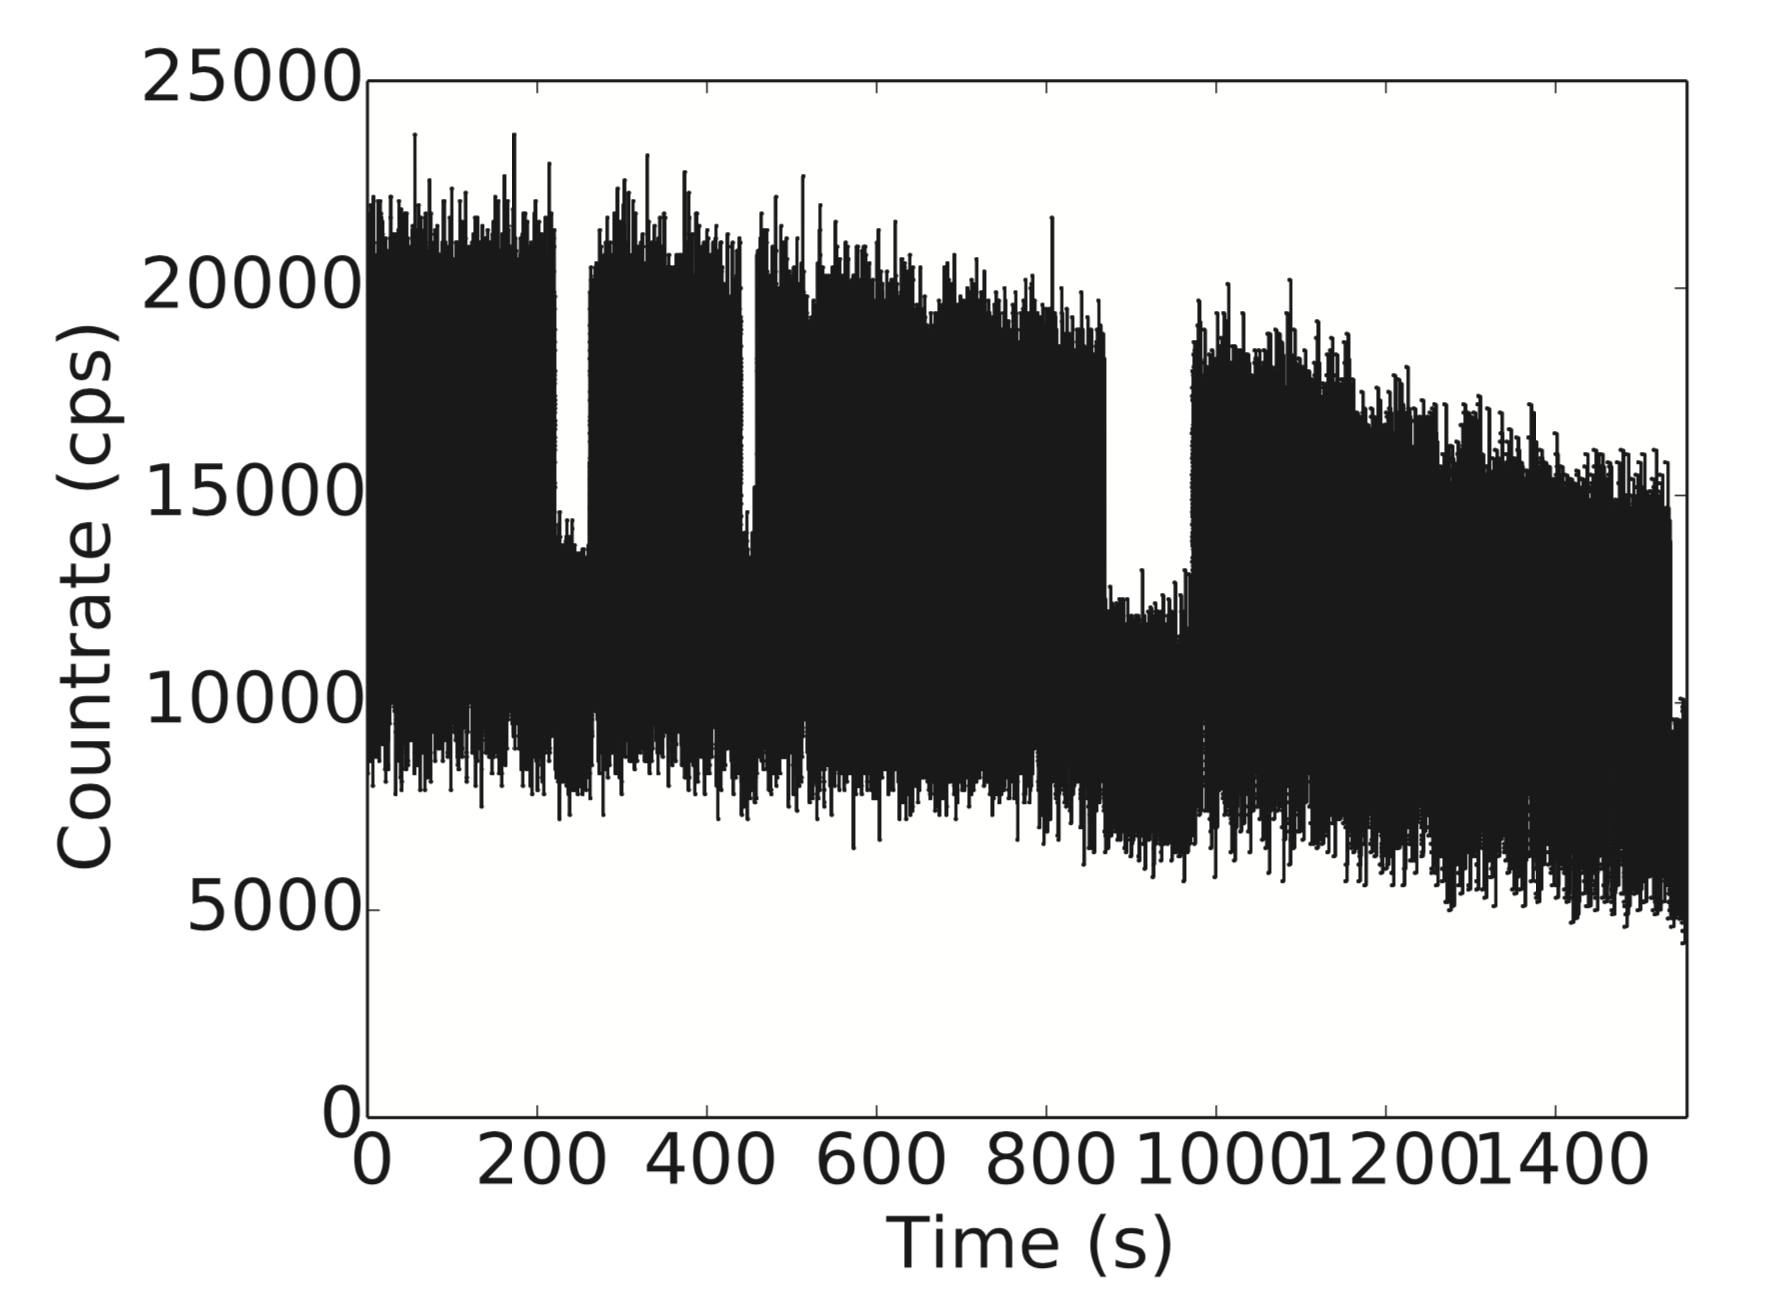
\includegraphics[trim = 0 0 0 0,  clip= true, width = \pairplotwide]{./pics/g2zuSpektrum8_15_5_countrate_0_01_conv_screenshot.png}}
				\caption{}\label{subfig::blink_long}
			\end{subfigure}
			\hfill
			\begin{subfigure}[tp]{ 0.49\linewidth}
				\centering
				\testbox{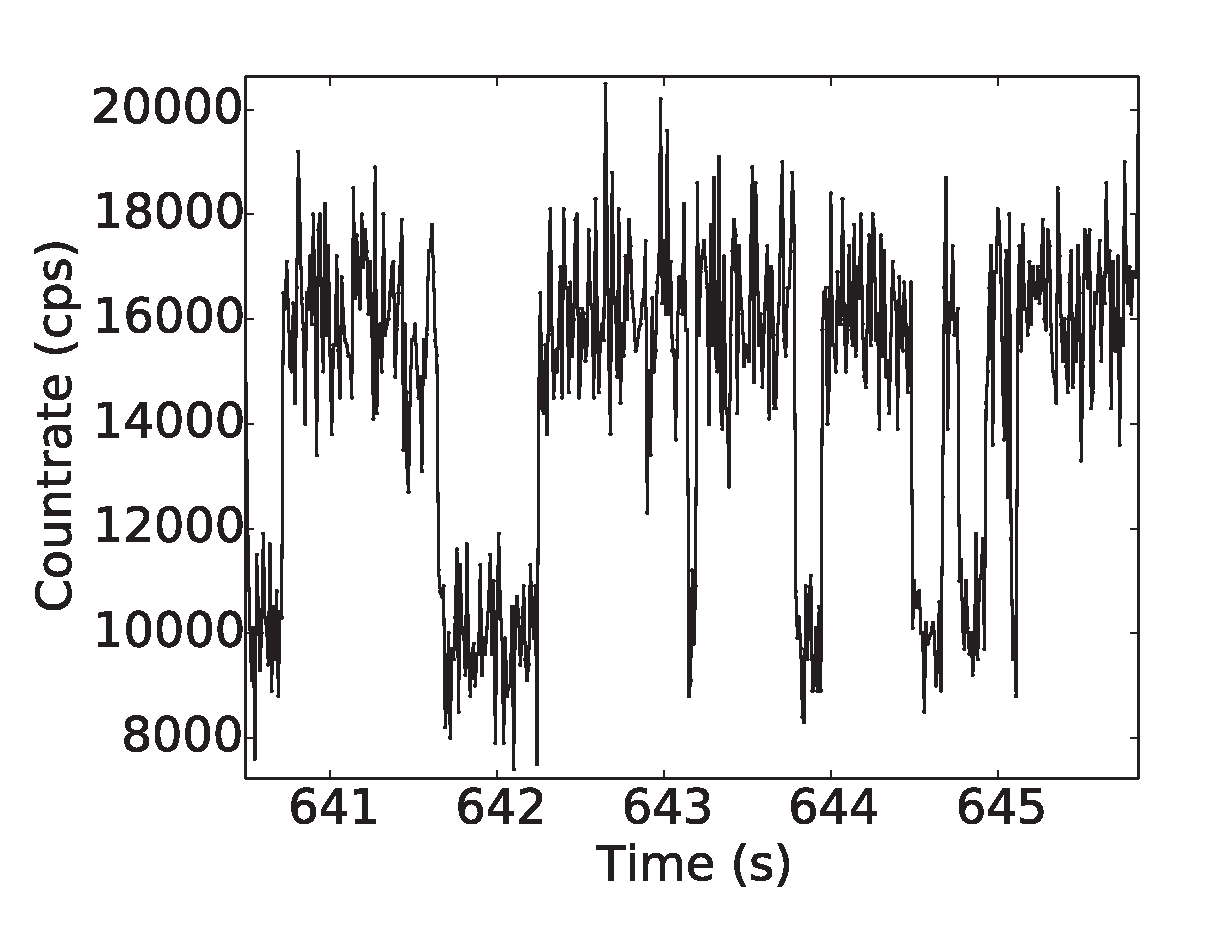
\includegraphics[trim = 0 0 0 0,  clip= true, width =\pairplotwide]{./pics/g2zuSpektrum8_15_5_countrate_0_01_conv_detail.pdf}}
				\caption{}\label{subfig::blink_short}
			\end{subfigure}
			\caption[Time trace of a single emitter.]{(a) Time trace of the single emitter H1, which exhibits strong blinking. The variation of the count rate in the upper state is attributed to a drift of the setup. (b) Detail of the time trace of the same emitter.}
			\label{fig::blink}
		\end{figure}

		The photon count time trace of emitter \emnarrow is shown in \Fref{fig::blink}.
		In the overview picture (\Fref{subfig::blink_long}), a few blinking dips can be seen with time intervals of up to a few minutes.
		The fact that the count rate never drops down to the dark count rate lets us assume, that there are at least two \sivs present, one exhibiting fluorescence intermittence and one exhibiting a stable emission.
		When zooming in, shorter time intervals are observable (\Fref{subfig::blink_short}).
		The time intervals range from a few tens of milliseconds up to a few seconds with a few outliers exhibiting very long time intervals up to a few hundred seconds.
		\\
		The bright and dark times exhibit different probability distribution functions and with that, different characteristic time constants.
		In \Fref{fig::fit_blink_distr} the time intervals of the emitter are shown as small vertical dashed red lines and solid blue lines for the bright and dark state respectively.

		\begin{figure}[!htb]
			\centering
			\testbox{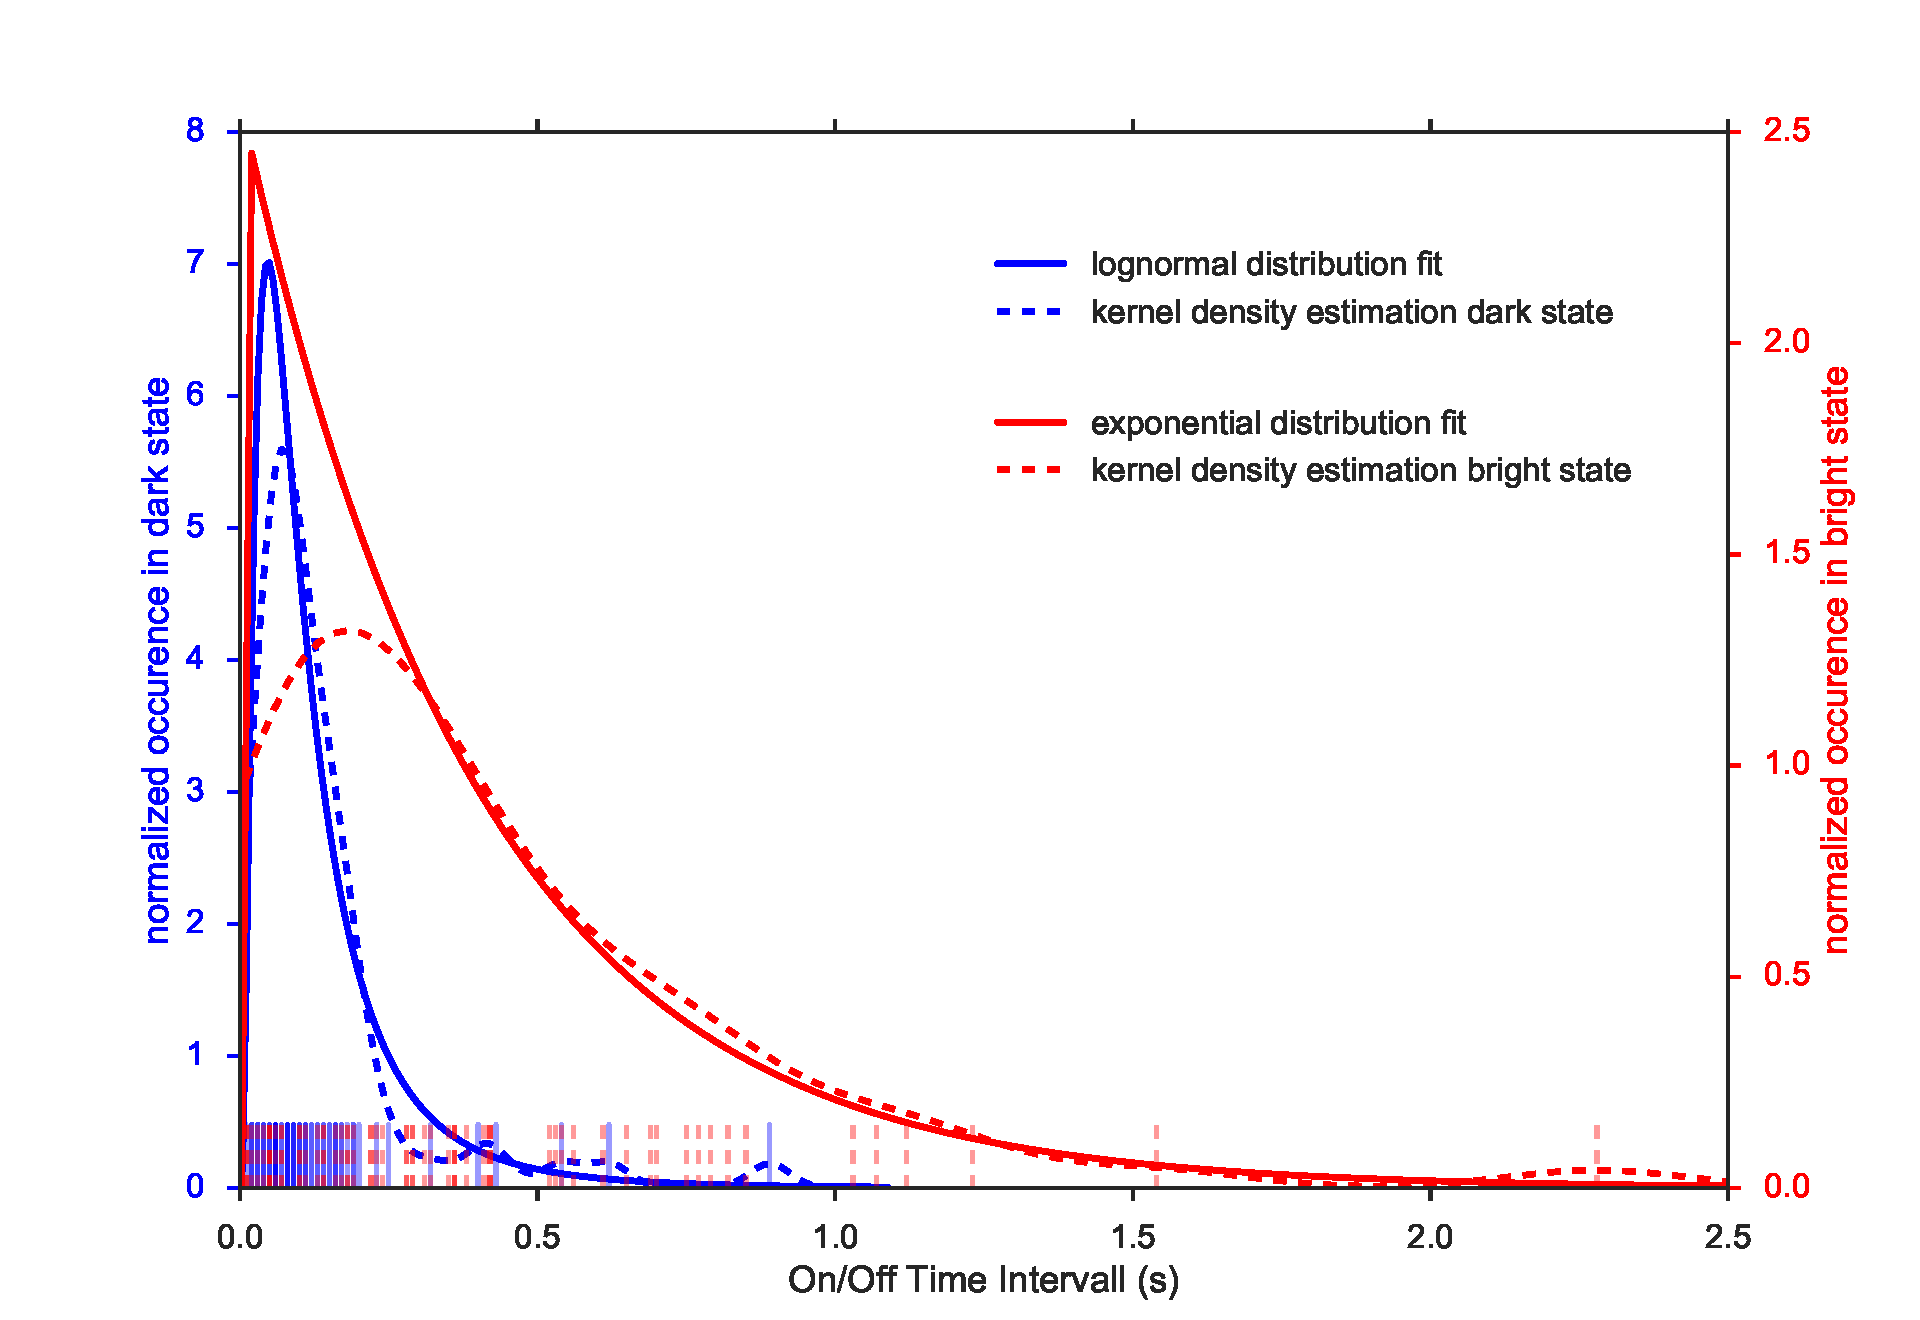
\includegraphics[trim = 0 0 0 0,  clip= true, width = \oneimagewide]{./pics/retention_no_histo_xlim2_5.pdf}}
			\caption[Distributions of brigth and dark state intervals]{Time intervals of the single emitter exhibiting the highest blinking rate in the bright (red) and dark (blue) states. Each flank of the blinking state was individually read out from the \pl time trace. On the horizontal axis small vertical lines represent the individual data points of the bright/dark time intervals. The blue and red dashed curves represent kernel density estimations of the distribution of time intervals of the dark and bright states, respectively. The y-axis is scaled to the normalized kernel density estimate. The red solid line is an exponential fit of the bright state time intervals whereas the blue solid line is a log-normal fit of the dark state time intervals. These fitting functions were chosen because they provide the best agreement with the data using a Kolomogorov-Smirnov test with respect to other functions (p-values: bright state (red) 0.92, dark state (blue) 0.77).}
			\label{fig::fit_blink_distr}
		\end{figure}

		Outliers with very long time intervals are ommited here.
		The dashed lines are kernel density estimators of the distribution of the respective time intervals.
		This implies that every data point is represented with a Gaussian function and the resulting functions are added up to model the whole data.
		The red solid line is an exponential fit of the distribution of time intervals in the bright state.
		The high p-value of \num{0.92} confirms the goodness of the fit.
		The median time interval in the bright state obtained by the exponential fit amounts to \SI[separate-uncertainty]{0.09}{s}.
		While other literature about solid state quantum emitters reports an exponential probability distribution for both time intervals in bright and dark states\cite{Bradac2010,Berhane2017}, we found a log-normal probability distribution for the time interval in the dark state.
		The solid blue line in \Fref{fig::fit_blink_distr} is a log-normal fit of the distribution of the time intervals in the dark state.
		A Kolomogorov-Smirnov test yields a p-value of \num{0.77} for the log-normal fit and is by far the best model to describe the data distribution.
		For comparison: The p-value of an exponential fit amounts to \num{0.36}.
		The median time interval in the dark state obtained by the log-normal fit is determined as \SI{0.10}{s}, therefore being close to the median time interval in the bright state.
		Very long time intervals are not shown in the plot for better visualization of the small timescales, however these long time intervals are included in the fit.
		The longest measured time interval amounted to \SI{41.14}{s} and occurred in the dark state.
		\\
		Measurements of blinking time intervals in \cite{Jantzen2016} and \cite{Neu2012a} report time intervals between about \SIrange{0.03}{1}{s}, and \SI{0.1}{s} to \SI{2}{min}, respectively.
		These findings are in good agreement with our measurements.
		\\
		In general, excitation and emission process is mediated by charge separation (i.e.\ excitons).
		If an electron or hole is localized far enough that there is sufficiently negligible overlap with the wave function of the remaining carrier, blinking occurs \cite{Efros2016}.
		We explain the observed blinking as a manifestation of the local crystal disorder due to dislocations and impurities which act as a trap for the excited electron and therefore switch the emitter to the dark state.
		The capture of the electron of the exciton by traps due to local crystal disorders may inhibit recombination and therefore induce the dark state \cite{Bradac2010}.
		The assumption that dislocations and impurities are responsible for blinking emitters is in agreement with our findings reported in \ref{ch::crystal_quality}.
		\\
		Research of blinking rhodamine molecules confirms power law distributed bright state times and log-normal distributed dark state times \cite{Wong2013}.
		The log-normal distribution is explained by a Gaussian distribution of activation barriers of the electron transfer to trap states in the surrounding material \cite{Albery1985}.
		It hints towards a recapture of the electron via multiphonon relaxation channels.

